\documentclass{lib/skripsi}

\usepackage{blindtext}
\usepackage{pdfpages}

%===========================================================
% Definisi Data Peneliti, Judul, Pembimbing dan Penguji
%-----------------------------------------------------------
\titleskripsi{Implementasi \textit{Pose Estimation} untuk Pemodelan Gerak Tari Tradisional Indonesia pada Robot \textit{Humanoid} Tari Robotis OP3}

\fullname{Aido Luthfi Al Hakim}
\idnum{2141720136}

\monthsubmit{Juli}
\yearsubmit{2025}
\datesubmit{16 Juli 2025}
\program{Teknik Informatika}
\dept{Teknologi Informasi}
\faculty{Teknik}
\university{Politeknik Negeri Malang}
\city{Malang}

\firstsupervisor{Wilda Imama Sabilla, S.Kom., M.Kom.}
\firstsupervisorNIP{19920829 201903 2 023}
\secondsupervisor{Ariadi Retno Tri Hayati Ririd, S.Kom., M.Kom.}
\secondsupervisorNIP{19810810 200501 2 002}



\firstexaminer{-}
\firstexaminerNIP{-}
\secondexaminer{-}
\secondexaminerNIP{-}
\headprogram{Ely Setyo Astuti, S.T., M.T.}
\headprogramNIP{19760515 200912 2 001}
\headdepartment{Prof. Dr. Eng. Rosa Andrie Asmara, S.T., M.T.}
\headdepartmentNIP{19801010 200501 1 001}
%-----------------------------------------------------------
% End Definisi Data Peneliti, Judul, Pembimbing dan Penguji
%===========================================================

\begin{document}
    % Cover page
    \pagenumbering{roman} % Start Roman numbering
    \pagestyle{roman} % Apply Roman style
    \cover

    % Approval page
    \clearpage
    \phantomsection
    \addcontentsline{toc}{chapter}{LEMBAR PENGESAHAN}
    lembar pengesahan
    \thispagestyle{roman}
    \newpage
    % \approvalpage
    % % 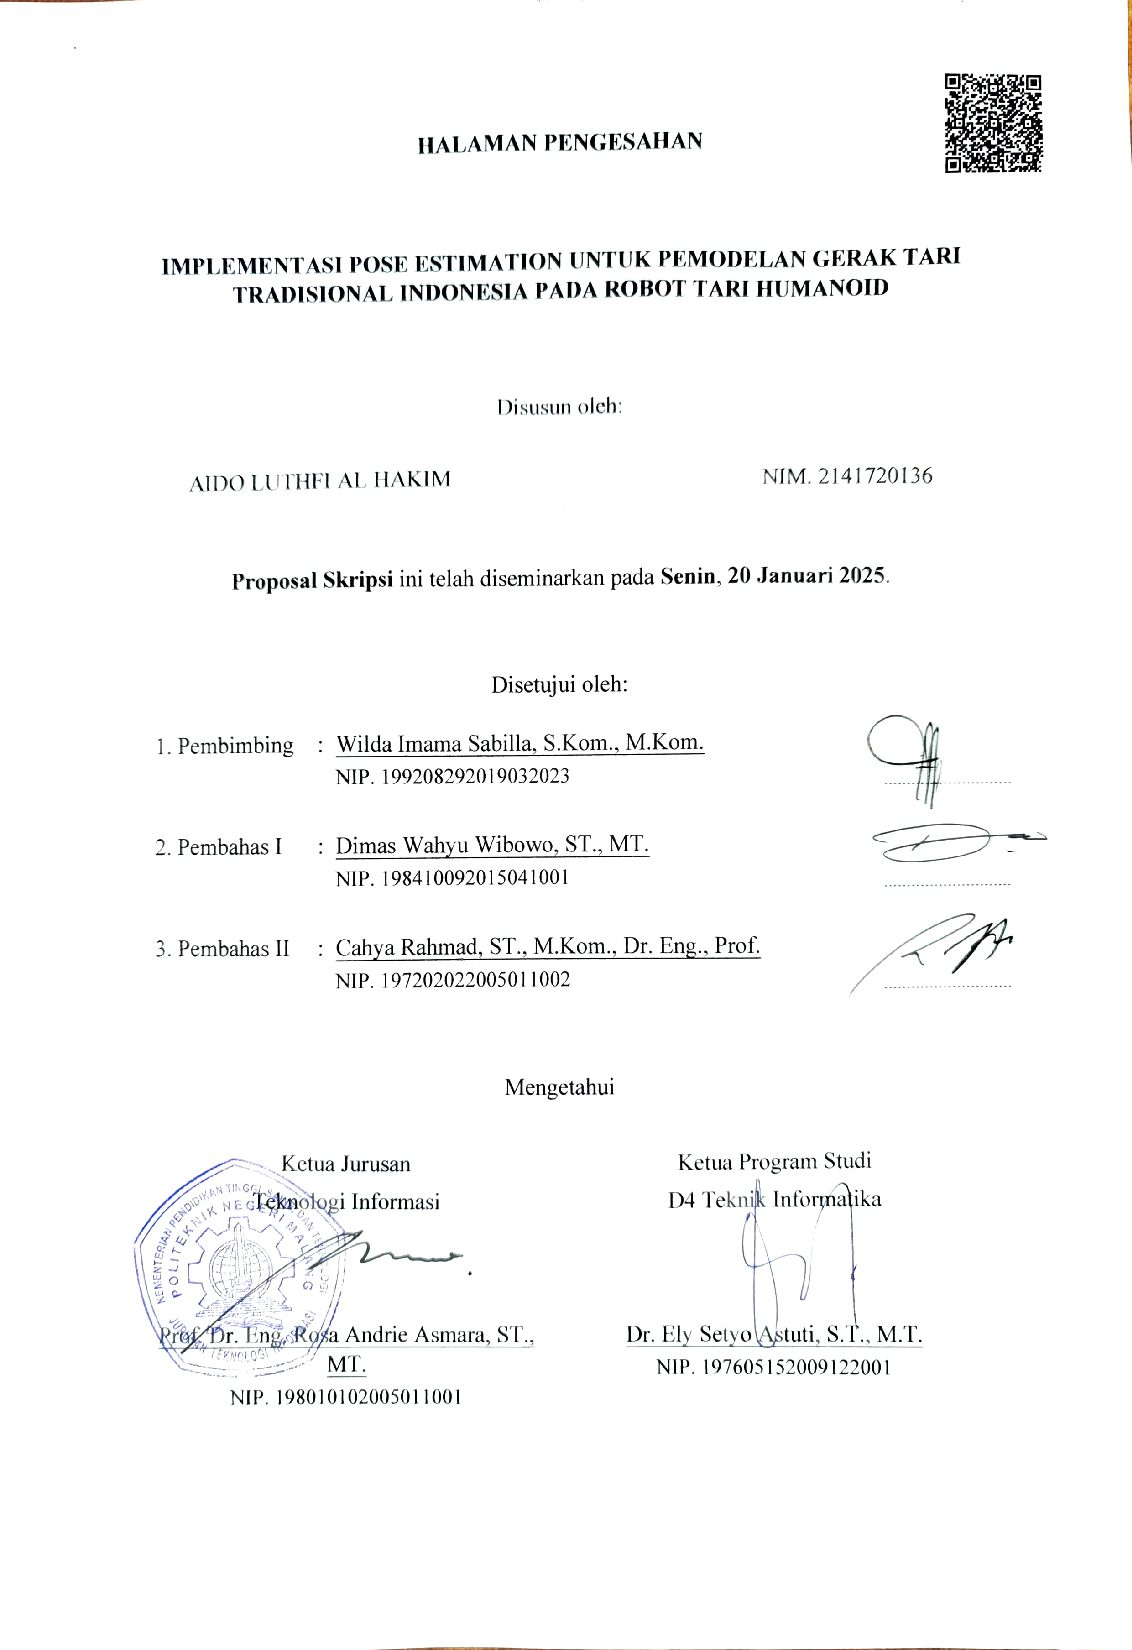
\includepdf[pages=-]{include/lembar-pengesahan.pdf}

    %===========================================================
    % Daftar isi, daftar gambar, daftar tabel
    %-----------------------------------------------------------
    % \clearpage
    % Authentication page
    \phantomsection
    \addcontentsline{toc}{chapter}{PERNYATAAN}
    \authenticationpage
    \clearpage

    % Abstract page
    \phantomsection
    \thispagestyle{roman}
    \abstractID{
    Perkembangan teknologi robotika membuka peluang bagi inovasi dalam berbagai bidang, termasuk pelestarian budaya melalui media robot \textit{humanoid}. Salah satu penerapannya adalah pada Kontes Robot Seni Tari Indonesia (KRSTI), di mana robot diharuskan menampilkan gerakan tari tradisional secara natural dan sesuai dengan irama musik. Namun, pembuatan gerakan tari pada robot \textit{humanoid} saat ini masih dilakukan secara manual sehingga tidak efisien. Penelitian ini mengembangkan sistem \textit{pose estimation} untuk pemodelan gerak tari tradisional Indonesia pada robot \textit{humanoid} ROBOTIS-OP3. Sistem menggunakan model \textit{Metrabs} untuk deteksi pose 3D dan \textit{DeciWatch} untuk penyempurnaan prediksi temporal. Pengujian pada gerakan T-pose dan tari Denok Semarangan menunjukkan penurunan MPJPE dari 107 mm menjadi 64{,}98 mm, dengan \textit{loss} sebesar 0{,}1522 dan waktu pelatihan 50 jam menggunakan \textit{custom training}. Sistem ini mendukung pelestarian budaya berbasis teknologi.
    }

    \keywordsID{Pose Estimation, Robot Humanoid, OP3, Gerak Tari}
    \abstractpageID
    \clearpage
    % Abstract page in English
    \phantomsection
    \thispagestyle{roman}
    \abstractEN{
    The development of humanoid robots provides opportunities for cultural preservation through robotic dance performance. However, creating dance movements for humanoid robots is still mostly done manually, resulting in inefficiency and time-consuming processes. This research develops a \textit{pose estimation} system for modeling Indonesian traditional dance movements on the ROBOTIS-OP3 robot. The system utilizes \textit{Metrabs} for 3D pose detection and \textit{DeciWatch} for temporal refinement. The output is converted into servo joint angles using \textit{Trigonometric Inverse Kinematics} with \textit{motion retargeting}. Tests on T-pose and Denok Semarangan dance show a reduction in MPJPE from 107 mm to 64.98 mm, with loss of 0.1522 and 50 hours of \textit{custom training}. This system promotes technology-based cultural preservation.
    }


    \keywordsEN{Pose Estimation, Humanoid Robot, OP3, Dance Movement}
    \abstractpageEN
    \clearpage

    % preface
    \phantomsection
    \prefacepage


    % Table of contents
    \phantomsection
    \addcontentsline{toc}{chapter}{DAFTAR ISI}
    \tableofcontents
    \clearpage

    % List of figures
    \phantomsection
    \addcontentsline{toc}{chapter}{DAFTAR GAMBAR}
    \listoffigures
    \clearpage

    % List of tables
    \phantomsection
    \addcontentsline{toc}{chapter}{DAFTAR TABEL}
    \listoftables
    \clearpage

    \phantomsection
    \addcontentsline{toc}{chapter}{DAFTAR LAMPIRAN}
    \listofappendices
    \clearpage

    % Main content
    \pagenumbering{arabic} % Switch to Arabic numbering
    \pagestyle{fancy} % Apply main chapter style

    %-----------------------------------------------------------
    % End Daftar isi, daftar gambar, daftar tabel
    %===========================================================
    \makeatletter
    \let\ps@plain\ps@chapterplain % Apply the "chapterplain" style to chapter title pages
    \makeatother
    %===========================================================
    % Daftar masukan untuk Bab
    %-----------------------------------------------------------
    \setlength{\parskip}{0pt} % jarak antar paragraf
    \chapter{PENDAHULUAN}
\vspace{1em}

\section{Latar Belakang}
Kemajuan teknologi semakin berkembang pesat dalam kehidupan manusia saat ini, terutama dengan adanya internet yang semakin luas dan mudah diakses. Hal ini membuka peluang besar bagi inovasi di berbagai bidang, termasuk pengembangan dalam bidang robotika. Salah satu cabang robotika yang menarik perhatian adalah robot \textit{humanoid} yaitu robot yang memiliki struktur menyerupai manusia, seperti kepala, tangan, badan, dan kaki, serta mampu meniru sejumlah pergerakan manusia \cite{jalil2016rancang}.

Teknologi robotika di Indonesia sudah banyak diaplikasikan sebagai teknologi yang mempermudah pekerjaan manusia terutama dalam bidang industri. Tidak hanya itu, kompetisi robot di Indonesia juga sering diselenggarakan untuk mendorong inovasi dan kreativitas mahasiswa serta pelajar dalam bidang robotika. Salah satu acara yang paling dikenal adalah Kontes Robot Indonesia (KRI) yang diselenggarakan oleh Balai Pengembangan Talenta Indonesia (BPTI). Kontes ini rutin diadakan setiap tahun untuk mengukur kemampuan mahasiswa dalam mendesain dan mengendalikan robot sesuai tema dan tantangan tertentu. KRI memiliki dua divisi yang melibatkan robot \textit{humanoid} yakni untuk melakukan misi bermain sepak bola pada Kontes Robot Sepak Bola Indonesia Humanoid (KRSBI-H) dan melakukan seni tari pada Kontes Robot Seni Tari Indonesia (KRSTI).

Robot \textit{humanoid} yang digunakan pada KRSTI merupakan robot yang dapat melakukan tarian tradisional Indonesia dengan tema yang telah ditentukan. Dalam mencapai misinya, robot tentu harus menghayati dan bergerak sesuai dengan tarian dan musik aslinya \shortcite{imania2023identifikasi}. Pergerakan robot \textit{humanoid} dalam melakukan tarian masih dilakukan secara manual dengan menggerakkan setiap sendi robot untuk setiap pergerakan tari. Hal tersebut menyebabkan sulitnya pembuat gerakan untuk menerapkan gerakan yang diinginkan pada robot karena memakan banyaknya repetisi pada pergerakan serta pemborosan waktu.

Dalam ajang KRSTI, setiap robot dalam kompetisi ini harus menampilkan tarian terbaik sesuai dengan tema tarian yang telah ditentukan. Salah satu kriteria penilaian utama adalah kemampuan robot untuk menari dan bergerak selaras dengan irama musik pengiring tema tarian tersebut. Selain itu, dua robot yang berpartisipasi harus dapat menari secara sinkron. Dalam ajang tersebut, Politeknik Negeri Malang telah beberapa kali berhasil lolos ke babak nasional. Namun, dalam pembuatan gerakan pada robot \textit{humanoid}, khususnya untuk tarian, prosesnya masih dilakukan secara manual. Hal ini menyebabkan kesulitan dalam menciptakan gerakan yang sesuai dengan keinginan, karena membutuhkan banyak repetisi pergerakan serta memakan waktu yang cukup lama, sehingga kurang efisien.

Untuk mengatasi permasalahan tersebut, salah satu solusi yang dapat diterapkan adalah teknologi pose estimation. Teknologi ini memungkinkan robot \textit{humanoid} untuk melakukan gerakan tarian secara otomatis melalui analisis visual dari gerakan manusia yang direkam menggunakan kamera. DeciWatch adalah salah satu metode canggih dalam estimasi pose manusia 2D/3D yang memanfaatkan pendekatan inovatif berbasis \textit{transformers}. Dengan pendekatan \textit{sample-denoise-recover}, DeciWatch secara efisien hanya menggunakan 10\% frame video untuk estimasi, mengurangi \textit{noise} pada data dengan DenoiseNet, dan merekonstruksi pose yang tidak diamati menggunakan RecoverNet yang memanfaatkan korelasi spasial dan temporal. Metode ini mampu menghasilkan estimasi pose manusia yang lebih akurat, presisi, dan halus, menjadikannya solusi ideal untuk menghasilkan gerakan robot \textit{humanoid} yang lebih natural dan efisien.

Dengan pose estimation, titik-titik kunci pada tubuh manusia, seperti sendi dan anggota tubuh, dapat diidentifikasi dan diterjemahkan ke dalam data koordinat yang digunakan untuk memprogram gerakan robot. Proses ini tidak hanya mengurangi kebutuhan repetisi manual, tetapi juga meningkatkan efisiensi waktu dalam pembuatan gerakan. Selain itu, pose estimation memungkinkan robot untuk menghasilkan gerakan yang lebih halus dan natural, sehingga performa robot dalam menari dapat ditingkatkan secara signifikan. Dengan penerapan teknologi ini, diharapkan robot \textit{humanoid} dapat lebih mudah memenuhi kriteria penilaian pada ajang seperti KRSTI. 


\section{Rumusan Masalah}
Berdasarkan uraian pada latar belakang diatas, permasalahan utama yang akan diangkat dalam penelitian ini adalah sebagai berikut:

\begin{itemize}
    \item Bagaimana memanfaatkan teknologi pose estimation untuk menganalisis gerakan manusia dan menghasilkan data pose dalam format 3D?
    \item Bagaimana mengaplikasikan data pose 3D yang dihasilkan oleh pose estimation untuk memprogram gerakan robot \textit{humanoid} tari agar dapat meniru gerakan manusia?
    \item Bagaimana merancang aplikasi yang dapat mengintegrasikan proses perekaman gerakan dan implementasi gerakan pada robot \textit{humanoid} tari dalam satu sistem berbasis website?
    \item Bagaimana mengevaluasi hasil \textit{pose estimation} dan implementasi gerakan pada robot \textit{humanoid} tari yang telah dibangun?
\end{itemize}

\section{Batasan Masalah}
Dari rumusan masalah diatas dapat dibuat suatu batasan-batasan masalah sebagai berikut:
\begin{itemize}
    \item Robot diam di tempat tanpa pergerakan translasi atau rotasi pada bagian kaki.
    \item Sistem memanfaatkan \textit{Robot Operating System (ROS)} dengan bahasa pemrograman Python sebagai media komunikasi dan pengendalian sebagian pergerakan robot.
    \item Pergerakan yang direplikasi hanya terbatas pada badan bagian atas, yaitu pergerakan lengan dan kepala, tanpa melibatkan sinkronisasi dengan musik.
    \item Aplikasi pendukung dibangun berbasis \textit{website}, ditujukan untuk anggota tim robotik.
    \item \textit{Dataset training} yang digunakan merupakan dataset \textit{pose estimation} yang tersedia secara publik di internet, bukan data yang diambil secara mandiri.
\end{itemize}

\section{Tujuan}
Adapun tujuan dari dilakukannya penelitian ini adalah sebagai berikut:
\begin{itemize}
    \item Mengembangkan teknologi \textit{pose estimation} untuk menganalisis gerakan manusia dan menghasilkan data pose dalam format 3D secara akurat.
    \item Mengaplikasikan data pose 3D yang dihasilkan untuk memprogram gerakan robot \textit{humanoid} tari sehingga dapat meniru gerakan manusia dengan presisi.
    \item Merancang dan membangun aplikasi berbasis website yang mengintegrasikan proses perekaman gerakan dan implementasi gerakan pada robot \textit{humanoid} tari.
    \item Untuk mengetahui evaluasi hasil \textit{pose estimation} dan implementasi gerakan pada robot \textit{humanoid} tari yang telah dibangun.
\end{itemize}

\section{Manfaat}
Manfaat yang diharapkan dari penelitian ini adalah sebagai berikut:
\begin{itemize}
    \item Memberikan kontribusi dalam pengembangan teknologi robotika di Indonesia, khususnya dalam bidang robot \textit{humanoid} tari.
    \item Mempermudah proses pembuatan gerakan tarian robot \textit{humanoid}, sehingga lebih efisien dalam waktu dan tenaga.
    \item Meningkatkan daya saing Politeknik Negeri Malang dalam ajang kompetisi robotika, khususnya dalam bidang robot \textit{humanoid} tari.
    \item Menjadi referensi bagi peneliti selanjutnya dalam pengembangan teknologi pose estimation dan implementasi gerakan pada robot \textit{humanoid} tari.
\end{itemize}
    \chapter{LANDASAN TEORI}
\vspace{1em}

\section{Studi Literatur}
Penelitian ini didasarkan pada studi literatur yang relevan terhadap topik skripsi. Pada penelitian sebelumnya yang berjudul \textit{"Pemanfaatan Estimasi Pose Gerak pada Penari Trance dalam Ritual Adat Ngalaksa"} bertujuan untuk mendeteksi pose gerak penari yang mengalami trance dalam ritual adat Ngalaksa di Desa Wisata Rancakalong, Sumedang, Jawa Barat. Penelitian ini menggunakan metode visi komputer berbasis GluonCV untuk analisis data pose gerak para penari. \textit{Dataset} gerak tari dikumpulkan melalui observasi lapangan, wawancara dengan informan seperti Saehu dan peserta ritual, serta dokumentasi visual. Hasil penelitian menunjukkan bahwa model estimasi pose berhasil mendeteksi perbedaan gerak antara penari yang mengalami trance dan yang tidak, meskipun akurasi untuk penari trance cenderung lebih rendah dibandingkan penari lainnya. Contohnya, akurasi untuk penari trance perempuan adalah 0.537, lebih rendah dibandingkan dengan akurasi penari biasa yang mencapai 0.802 hingga 0.993. Temuan ini menyoroti perlunya pengembangan lebih lanjut untuk meningkatkan akurasi model dan mendukung pelestarian seni budaya nusantara dengan teknologi kecerdasan buatan.

Salah satu metode awal pada bidang estimasi pose adalah VNect yang merupakan hasil dari penelitian \textit{"VNect: Real-time 3D Human Pose Estimation with a Single RGB Camera"} yang diperkenalkan pada tahun 2017. Metode ini mampu mengestimasi pose 3D tubuh manusia secara global dan konsisten secara temporal dari input kamera RGB tunggal secara \textit{real-time}, metode ini berhasil menghasilkan model dengan akurasi \textit{mean per joint position error} (MPJPE) 80.5mm. Dengan menggunakan jaringan konvolusional (CNN), VNect meregresikan posisi \textit{joint} 2D dan 3D tanpa memerlukan \textit{bounding box} yang ketat. Hasil regresi dioptimalkan melalui \textit{kinematic skeleton fitting} untuk menghasilkan pose yang stabil secara temporal. Namun, metode ini rentan terhadap noise pada deteksi awal \textit{joint} 2D yang dapat memengaruhi estimasi 3D \cite{mehta2017vnect}.

Metode lain yang lebih terkini adalah \textit{"Deep High-Resolution Representation Learning for Human Pose Estimation"} yang dirancang untuk mempertahankan resolusi tinggi sepanjang proses estimasi pose manusia. Dengan menggunakan \textit{subnet} resolusi tinggi yang terhubung secara paralel dengan \textit{subnet} resolusi rendah, HRNet memungkinkan pertukaran informasi multi-skala yang berulang. Hasilnya, HRNet memberikan akurasi tinggi pada beberapa \textit{dataset}. Pada pengujian menggunakan metrik PCKh@0.5, HRNet mencapai nilai 90.3, yang menunjukkan performa luar biasa dalam estimasi pose manusia \shortcite{sun2019deep}.

Di sisi lain, tak hanya untuk \textit{text generation}, penggunaan \textit{transformer} pada visi komputer juga sudah berkembang pesat. Dalam penelitian berjudul \textit{"DeciWatch: A Simple Baseline for 10× Efficient 2D and 3D Pose Estimation"}, diperkenalkan kerangka kerja berbasis \textit{transformer} yang inovatif bernama DeciWatch. Model ini dirancang untuk meningkatkan efisiensi estimasi pose manusia 2D/3D hingga 10 kali lipat dibandingkan metode tradisional tanpa mengorbankan akurasi. Hasil eksperimen menunjukkan bahwa DeciWatch menghasilkan estimasi yang lebih halus dan akurat dengan biaya komputasi yang jauh lebih rendah. Model ini divalidasi pada beberapa dataset benchmark, seperti Human3.6M dan AIST++, dengan pencapaian performa tinggi dalam akurasi serta efisiensi komputasi. Sebagai contoh, DeciWatch berhasil mencapai MPJPE sebesar 52,8 mm pada Human3.6M dengan hanya menggunakan 10\% \textit{frame} video, mengungguli model sebelumnya dan tetap mempertahankan biaya komputasi yang minimal \cite{zeng2022deciwatch}.

Pada topik yang sama dengan penelitian ini yaitu imitasi gerakan manusia pada robot humanoid terdapat penelitian berjudul \textit{"Motion Imitation of a Humanoid Robot via Pose Estimation"}, memperkenalkan metode imitasi gerakan robot humanoid menggunakan estimasi pose 3D berbasis RGB-D. Penelitian ini memanfaatkan \textit{sparse tensor}, \textit{mask net}, dan \textit{sparsity pruning} untuk mengurangi konsumsi memori dan waktu komputasi. Dengan menerapkan \textit{motion retargeting} berbasis transformasi koordinat, robot NAO mampu meniru gerakan manusia secara akurat pada berbagai tugas, seperti meninju dan melambai \shortcite{10327198}. Eksperimen yang dilakukan menunjukkan bahwa metode ini menghasilkan imitasi gerakan yang stabil dan berkelanjutan. Untuk mengurangi getaran pada pergerakan robot, digunakan \textit{Kalman Filter} pada sudut sendi yang dihasilkan dari proses \textit{retargeting}. Hasil uji coba pada \textit{Berkeley MHAD dataset} menunjukkan tingkat kesalahan prediksi \textit{Mean Per Joint Position Error (MPJPE)} sebesar 27.72 mm untuk semua aksi, dan 20.04 mm pada tujuh aksi pertama yang lebih terlihat penuh tanpa occlusion. Hal ini membuktikan bahwa metode yang diajukan dapat menghasilkan performa estimasi pose dan imitasi gerak yang akurat meskipun menggunakan perangkat RGB-D yang lebih ekonomis dibandingkan sistem \textit{motion capture} konvensional. Dalam penelitian ini, robot NAO digunakan sebagai platform robotik, sedangkan dalam penelitian yang dilakukan oleh penulis, metode serupa diadaptasi dan diterapkan pada Robotis OP3, dengan menyesuaikan struktur mekanik dan aktuator yang berbeda namun dengan prinsip dasar pemetaan gerakan yang serupa.

Penelitian lain berjudul \textit{"Robust Regression-Based Motion Perception for Online Imitation on Humanoid Robot"} mengusulkan metode \textit{motion retargeting} berbasis \textit{robust regression} untuk memetakan gerakan manusia ke robot humanoid secara langsung. Proses pemetaan sudut dilakukan dengan perhitungan trigonometri menggunakan transformasi vektor spasial, melibatkan perhitungan \textit{shoulder pitch}, \textit{shoulder roll}, \textit{elbow yaw}, dan \textit{elbow roll}. Pendekatan ini memproyeksikan posisi sendi manusia ke sistem koordinat robot untuk mengontrol pergerakan lengan secara \textit{real-time}. Metode ini menjadi referensi dalam penelitian ini untuk diterapkan pada Robotis OP3, dengan penyesuaian pada struktur dan aktuator robot \cite{robust2017imitation}.

Selain itu, penelitian \textit{"Mixed Reality Interface for Whole-Body Balancing and Manipulation of Humanoid Robot"} memperkenalkan antarmuka \textit{mixed reality } (MR) untuk teleoperasi robot ROBOTIS-OP3. Dengan memanfaatkan teknologi \textit{motion retargeting} berbasis perhitungan skala linier dan \textit{inverse kinematics}, operator dapat mengontrol robot tanpa kontroler tambahan. Sistem ini juga memungkinkan pemantauan stabilitas robot melalui \textit{augmented view} yang menampilkan posisi \textit{center of mass} dan \textit{balanced state basin} \shortcite{song2024mixed}.

\begin{longtable}{cp{3.7cm}p{2cm}p{5cm}}
    \caption{Tabel Studi Literatur} \label{tab:ringkasan_artikel} \\

    \hline
    \textbf{No} & \multicolumn{1}{c}{\textbf{Judul}} & \multicolumn{1}{c}{\textbf{Metode Penelitian}} & \multicolumn{1}{c}{\textbf{Hasil Penelitian}} \\ \hline
    \endfirsthead

    \hline
    \textbf{No} & \multicolumn{1}{c}{\textbf{Judul}} & \multicolumn{1}{c}{\textbf{Metode Penelitian}} & \multicolumn{1}{c}{\textbf{Hasil Penelitian}} \\ \hline
    \endhead

    \hline
    \endfoot

    \hline
    \endlastfoot
    1 & \textit{"Pemanfaatan Estimasi Pose Gerak pada Penari Trance dalam Ritual Adat Ngalaksa"} \cite{listiani2024pemanfaatan}& Estimasi pose menggunakan GluonCV, visi komputer, analisis data visual & Model estimasi pose berhasil mendeteksi perbedaan gerak antara penari trance dan tidak trance dengan akurasi 0.537 untuk penari trance perempuan, dan akurasi 0.802--0.993 untuk penari biasa. \\ \hline
    2 & \textit{"VNect: Real-time 3D Human Pose Estimation with a Single RGB Camera"} \cite{mehta2017vnect}& CNN, \textit{kinematic skeleton fitting} & Mengestimasi pose 3D secara global dan temporal dengan input kamera webcam, stabil tetapi rentan terhadap \textit{noise} pada deteksi awal \textit{joint}. \\ \hline
    3 & \textit{"Deep High-Resolution Representation Learning for Human Pose Estimation"} \cite{sun2019deep} & HRNet (\textit{Parallel Multi- resolution Subnetworks}) & Akurasi tinggi pada estimasi pose dengan resolusi tinggi, unggul pada \textit{dataset} COCO dan MPII dibandingkan metode Resnet. \\ \hline
    4 & \textit{"DeciWatch: A Simple Baseline for 10× Efficient 2D and 3D Pose Estimation"} \cite{zeng2022deciwatch} & estimasi pose menggunakan pendekatan \textit{sample-denoise- recover}, transformer, dan \textit{DenoiseNet- RecoverNet} & Model berhasil meningkatkan efisiensi estimasi pose hingga 10× lebih cepat dengan akurasi MPJPE 52,8 mm pada \textit{dataset} Human3.6M, serta efisiensi komputasi yang signifikan. \\ \hline
    5 & \textit{"Motion Imitation of a Humanoid Robot via Pose Estimation"} \shortcite{10327198} & \textit{Sparse tensor}, \textit{mask net}, \textit{sparsity pruning}, \textit{motion retargeting} & Mengurangi konsumsi memori dan meningkatkan akurasi estimasi pose 3D pada robot \textit{humanoid} NAO. \\ \hline
    6 & \textit{"Robust Regression-Based Motion Perception for Online Imitation on Humanoid Robot"} \shortcite{robust2017imitation} & \textit{Robust regression}, \textit{motion retargeting}, trigonometri & Pemetaan sudut sendi manusia ke robot humanoid menggunakan transformasi vektor spasial dan perhitungan trigonometri secara \textit{real-time}. \\ \hline
    7 & \textit{"Mixed Reality Interface for Whole-Body Balancing and Manipulation of Humanoid Robot"} \cite{song2024mixed} & \textit{Mixed Reality} (MR), \textit{motion retargeting}, IK & Pengendalian robot \textit{humanoid} ROBOTIS-OP3 menggunakan \textit{Virtual Reality}. \\ \hline
\end{longtable}

\section{Dasar Teori}

\subsection{Robot \textit{Humanoid} Robotis-OP3}
Robotis-OP3 adalah robot \textit{humanoid} yang dikembangkan oleh Robotis, perusahaan yang dikenal dengan produk-produk robotika canggih untuk pendidikan, penelitian, dan otomasi. OP3 dirancang sebagai platform robot \textit{humanoid} dengan kemampuan tinggi, yang sering digunakan dalam penelitian robotika, termasuk bidang pemrosesan visual, estimasi pose, dan kontrol gerakan.

Secara umum, robot ini merupakan robot \textit{humanoid} yang dirancang untuk kompetisi robot sepak bola. Robot ini memiliki tinggi sekitar 51 cm dan berat 3,5 kg serta dilengkapi dengan 20 motor servo Dynamixel, terdiri dari 2 motor di kepala, 3 motor di setiap lengan, dan 6 motor di setiap kaki, yang mendukung gerakan artikulasi yang kompleks. Selain itu, OP3 memiliki kamera terintegrasi di bagian kepala untuk menangkap data visual, serta sensor IMU (\textit{Inertial Measurement Unit}) yang berfungsi untuk menjaga keseimbangan dan membantu navigasi \cite{damar2023football}.


\begin{figure}[H]
    \centering
    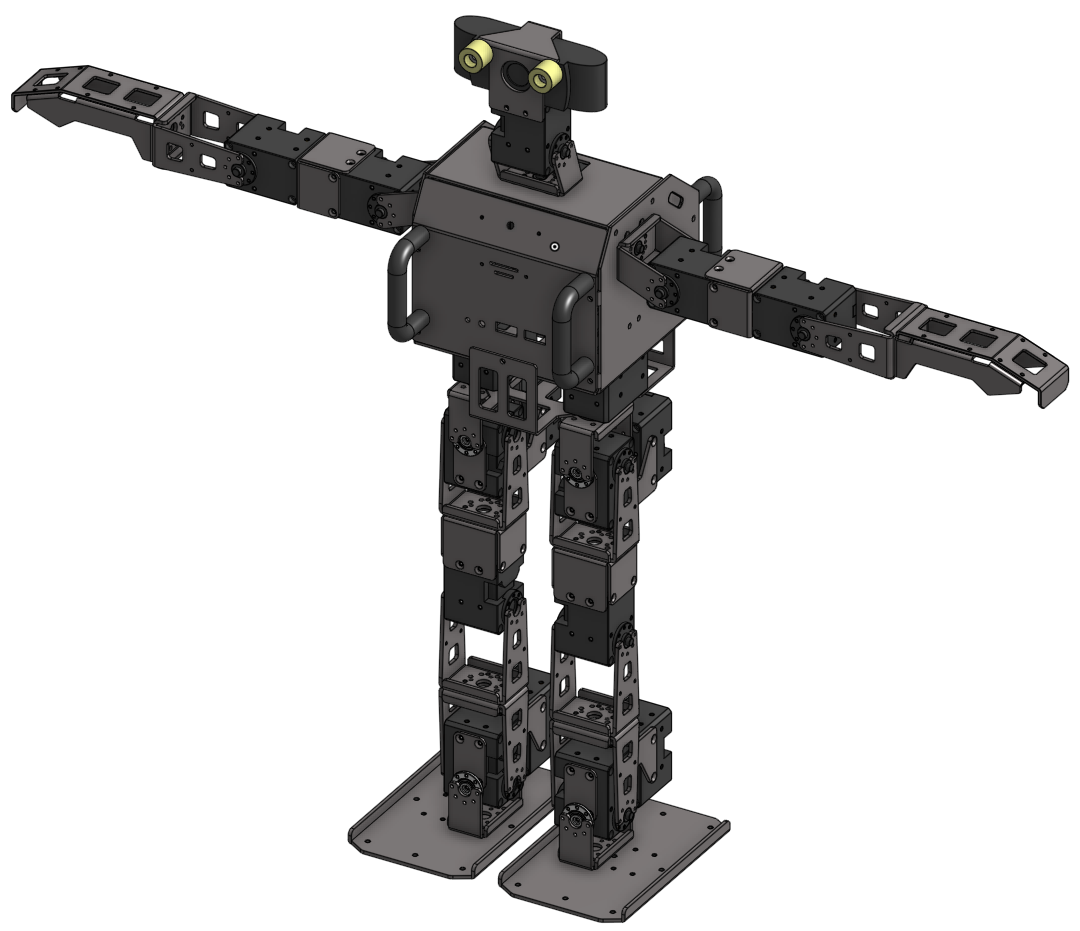
\includegraphics[width=0.45\textwidth]{images/robotis_op3.png}
    \captionsource{Robotis-OP3}{\cite{robotis_op3}}
    \label{fig:robotis_op3}
\end{figure}

\begin{figure}[H]
    \centering
    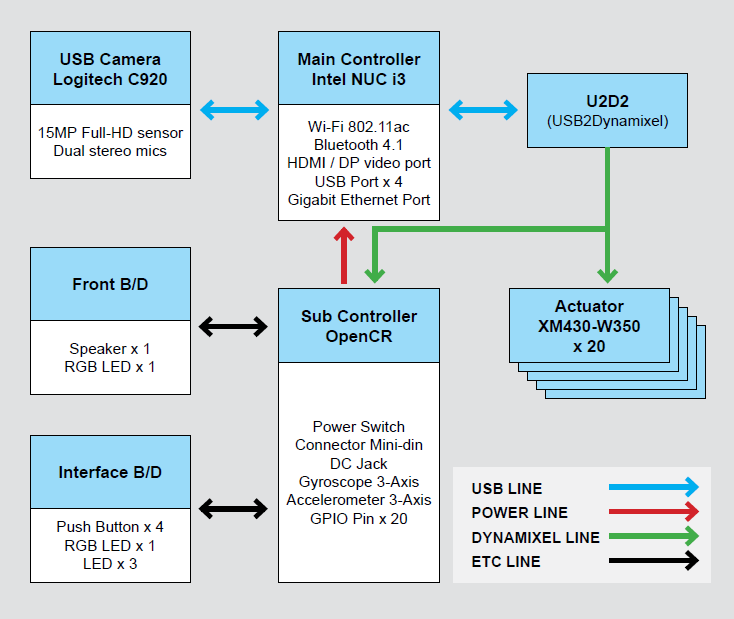
\includegraphics[width=0.6\textwidth]{images/op3_system.png}
    \captionsource{Sistem Robotis-OP3}{\cite{robotis_op3}}
    \label{fig:system_op3}
\end{figure}

\subsection{Dynamixel}

\textit{Dynamixel} adalah aktuator pintar yang dikembangkan oleh Robotis dan banyak digunakan pada sistem robotika modular, termasuk pada robot \textit{humanoid} seperti ROBOTIS-OP3. Berbeda dengan servo konvensional, Dynamixel memiliki fitur komunikasi dua arah yang memungkinkan pengguna tidak hanya mengendalikan sudut atau kecepatan, tetapi juga membaca data seperti posisi saat ini, beban, suhu, dan status error secara real-time \cite{robotis_dynamixel}.

Dynamixel menggunakan protokol komunikasi serial berbasis \textit{half-duplex} dengan dua metode utama, yaitu \textit{TTL} dan \textit{RS-485}. Pada ROBOTIS-OP3, komunikasi dengan servo dilakukan menggunakan protokol \textit{RS-485}, yang mendukung transmisi data jarak lebih jauh dan lebih stabil dibandingkan \textit{TTL}. Setiap servo dihubungkan secara daisy-chain melalui satu jalur komunikasi, sehingga memudahkan perakitan dan pengendalian banyak motor secara simultan \cite{robotis_manual}.

Untuk memudahkan integrasi dengan berbagai bahasa pemrograman, Robotis menyediakan \textit{Dynamixel SDK}, sebuah pustaka perangkat lunak yang mendukung pengendalian servo menggunakan bahasa C, C++, Python, Java, dan MATLAB. SDK ini memungkinkan pengiriman instruksi dan pembacaan data melalui API yang kompatibel dengan berbagai sistem operasi seperti Windows, Linux, dan macOS \cite{robotis_sdk}.

Pada platform ROBOTIS-OP3, terdapat dua jenis seri Dynamixel yang digunakan, yaitu XM430-W350-R dan 2XL430-W250-T. Dynamixel XM430-W350-R digunakan pada bagian kaki dan lengan robot karena memiliki torsi yang cukup besar serta mendukung berbagai mode kontrol seperti posisi, kecepatan, dan arus. Selain itu, motor ini juga dilengkapi dengan fitur \textit{current-based position control} yang memungkinkan pengendalian lebih presisi dan aman terhadap beban berlebih. Sementara itu, Dynamixel 2XL430-W250-T digunakan pada bagian kepala untuk menggerakkan dua sumbu sekaligus, yaitu \textit{yaw} dan \textit{pitch}, dalam satu modul motor. Modul ini memiliki dua port keluaran motor, sehingga lebih efisien dalam penggunaan ruang dan bobot, serta cocok untuk aplikasi di bagian kepala robot yang memerlukan mekanisme gerak ganda dengan dimensi yang lebih ringkas \cite{robotis_op3}.

\begin{figure}[H]
    \centering
    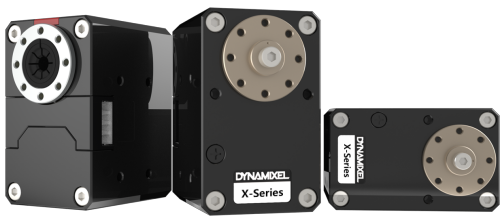
\includegraphics[width=0.6\textwidth]{images/dynamixel.png}
    \captionsource{Dynamixel X-Series}{\cite{robotis_dynamixel}}
    \label{fig:dynamixel}
\end{figure}


\subsection{\textit{Robot Operating System}}
\textit{Robot Operating System} (ROS) adalah \textit{framework} perangkat lunak untuk robotika yang menyediakan berbagai \textit{library} dan alat untuk memfasilitasi pengembangan aplikasi robot. ROS memungkinkan komunikasi antar modul perangkat keras dan perangkat lunak melalui arsitektur berbasis \textit{publish-subscribe} yang efisien, sehingga memudahkan integrasi berbagai komponen seperti sensor, aktuator, dan algoritma kontrol. Selain itu, ROS juga mendukung simulasi gerakan robot menggunakan platform seperti Gazebo, yang memungkinkan pengujian algoritma secara virtual sebelum diimplementasikan pada perangkat keras sebenarnya \cite{sa2024pengembangan}. Pada robot humanoid seperti ROBOTIS-OP3, ROS digunakan untuk berbagai fungsi, termasuk kontrol gerakan, visualisasi data sensor, pengolahan gambar, dan integrasi sistem secara keseluruhan, sehingga menjadi salah satu elemen kunci dalam pengembangan aplikasi robotik.

\subsection{Visi Komputer}
Visi Komputer adalah cabang ilmu komputer yang berfokus pada pengembangan algoritma dan teknik untuk memungkinkan komputer memahami dan mengekstrak informasi bermakna dari data visual seperti gambar, video, atau aliran data dari sensor visual lainnya. Bidang ini bertujuan untuk mensimulasikan kemampuan penglihatan manusia sehingga komputer dapat mengenali, menganalisis, dan membuat keputusan berdasarkan data visual \shortcite{marpaung2022computer}. Teknik dasar dalam visi komputer meliputi deteksi tepi, segmentasi objek, pengenalan fitur, dan estimasi pose. Deteksi tepi digunakan untuk menemukan batasan objek dalam gambar dengan mengidentifikasi perubahan intensitas yang signifikan, seperti yang dilakukan oleh algoritma \textit{Canny Edge Detection}. Segmentasi objek membagi gambar menjadi bagian-bagian yang lebih kecil atau objek tertentu untuk analisis lebih lanjut, menggunakan metode seperti \textit{thresholding} atau \textit{neural networks}. Pengenalan fitur bertujuan untuk mengekstrak elemen-elemen khas seperti sudut, garis, atau pola, yang penting untuk pelacakan atau pengenalan objek. Estimasi pose adalah proses menentukan posisi dan orientasi tubuh manusia atau objek dalam ruang 2D atau 3D, yang biasanya menggunakan algoritma berbasis jaringan saraf tiruan atau model regresi.


Dalam robotika, visi komputer memainkan peran penting dalam berbagai aplikasi. Salah satunya adalah navigasi robot, di mana data visual digunakan untuk mengenali lingkungan sekitar dan menentukan jalur optimal. Selain itu, deteksi lingkungan memungkinkan robot untuk mengidentifikasi rintangan atau area tertentu, membantu dalam penghindaran tabrakan atau penyelesaian tugas. Visi komputer juga digunakan untuk mengenali gerakan manusia, yang menjadi dasar bagi robot \textit{humanoid} dalam meniru gerakan tersebut. Salah satu penerapannya adalah dalam pemodelan gerakan kompleks, seperti gerakan tari atau aktivitas olahraga, yang membutuhkan analisis koordinasi tubuh secara terus-menerus \shortcite{kim2023human}.


\subsection{\textit{Deep Learning}}
Dalam dunia teknologi saat ini sudah tidak asing lagi dengan \textit{Artificial Intelligence} (AI). Perusahaan besar seperti Google, Microsoft, dan Meta saling berlomba untuk menciptakan \textit{Large Language Model} (LLM) seperti \textit{Gemma, Mistral,} dan \textit{Llama}. LLM merupakan salah satu aplikasi utama dari \textit{Deep Learning}, yang memungkinkan pemodelan teks secara kompleks dengan memahami konteks dan hubungan antar kata dalam skala besar.

\textit{Deep Learning} (DL) atau Pembelajaran Mendalam adalah salah satu cabang dari pembelajaran mesin yang berfokus pada pemodelan abstraksi tingkat tinggi pada data. Hal ini dilakukan dengan menggunakan sekumpulan fungsi transformasi non-linear yang ditata secara berlapis-lapis (\textit{deep neural networks}) dan mendalam \cite{ahmad2017mengenal}. DL sangat baik diterapkan pada \textit{supervised learning}, \textit{unsupervised learning}, \textit{semi-supervised learning}, maupun \textit{reinforcement learning} untuk berbagai aplikasi seperti pengenalan citra, pengenalan suara, klasifikasi teks, dan lainnya.

Model dalam DL pada dasarnya dibangun berdasarkan Jaringan Saraf Tiruan (\textit{Neural Network}), yang risetnya telah berlangsung sejak era 1980-an. Namun, DL baru kembali menjadi populer dengan kemajuan teknologi komputer yang semakin cepat, terutama berkat teknologi \textit{Big Data} seperti Hadoop dan Spark berbasis \textit{multi-node cluster}, serta pemrosesan secara paralel berbasis GPU. Jika suatu jaringan memiliki lebih dari tiga lapisan, maka jaringan tersebut dapat disebut sebagai \textit{Deep Network} \shortcite{cholissodin2020ai}.

DL memanfaatkan algoritma berbasis \textit{backpropagation} untuk mengoptimalkan bobot jaringan. Dalam konteks visi komputer, DL telah digunakan secara luas untuk tugas seperti klasifikasi gambar, deteksi objek, segmentasi, dan estimasi pose manusia. Selain itu, DL juga menjadi tulang punggung bagi pengembangan LLM, yang memungkinkan analisis teks secara kompleks dan menghasilkan teks yang menyerupai bahasa manusia.



\begin{figure}[h!]
    \centering
    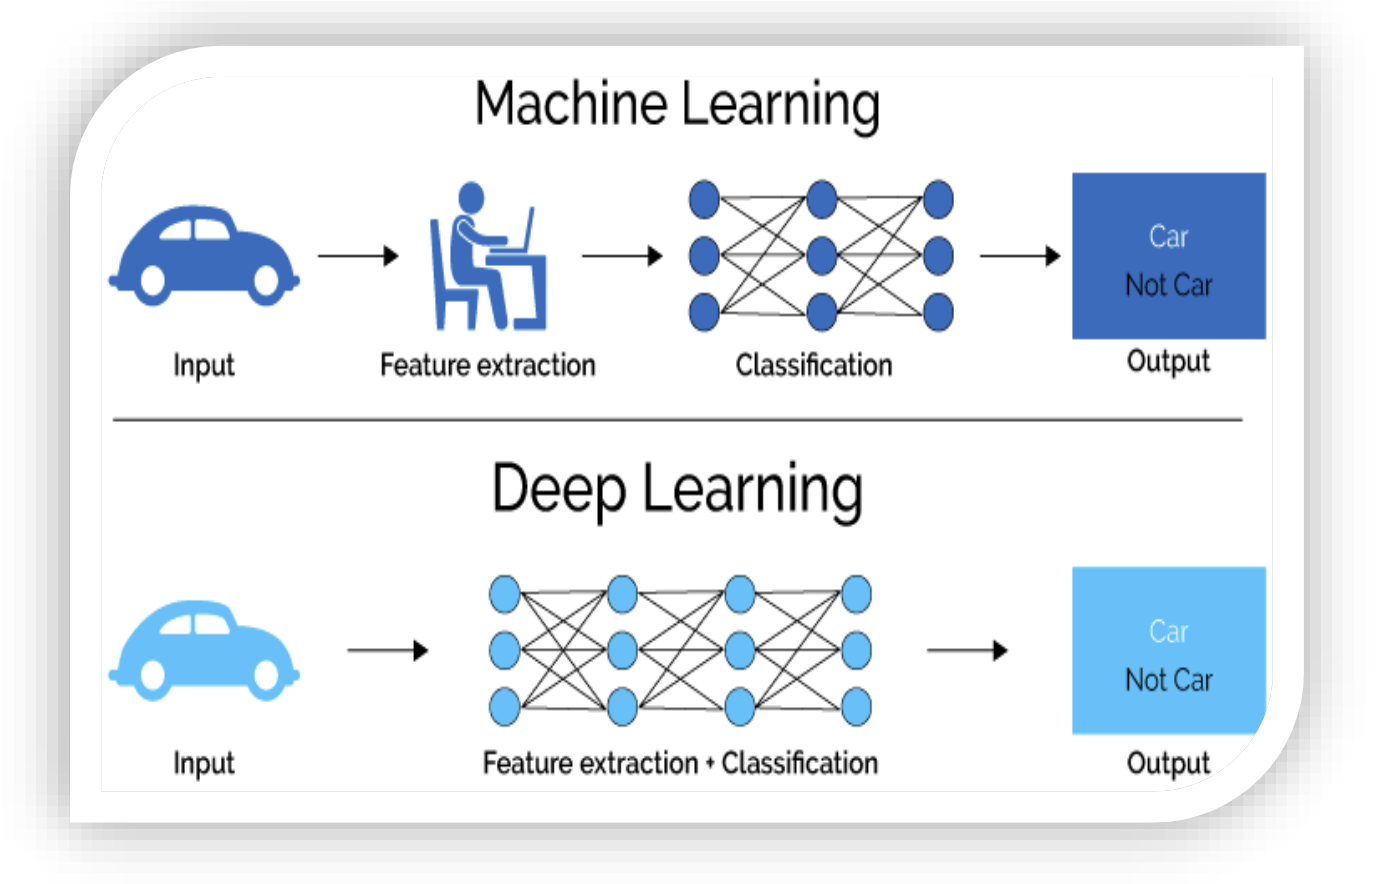
\includegraphics[width=0.5\textwidth]{images/deep_machine_diagram.png}
    \captionsource{Perbedaan ML dan DL}{\cite{cholissodin2020ai}}
    \label{fig:ai_ml_dl_llm}
\end{figure}

\begin{figure}[h!]
    \centering
    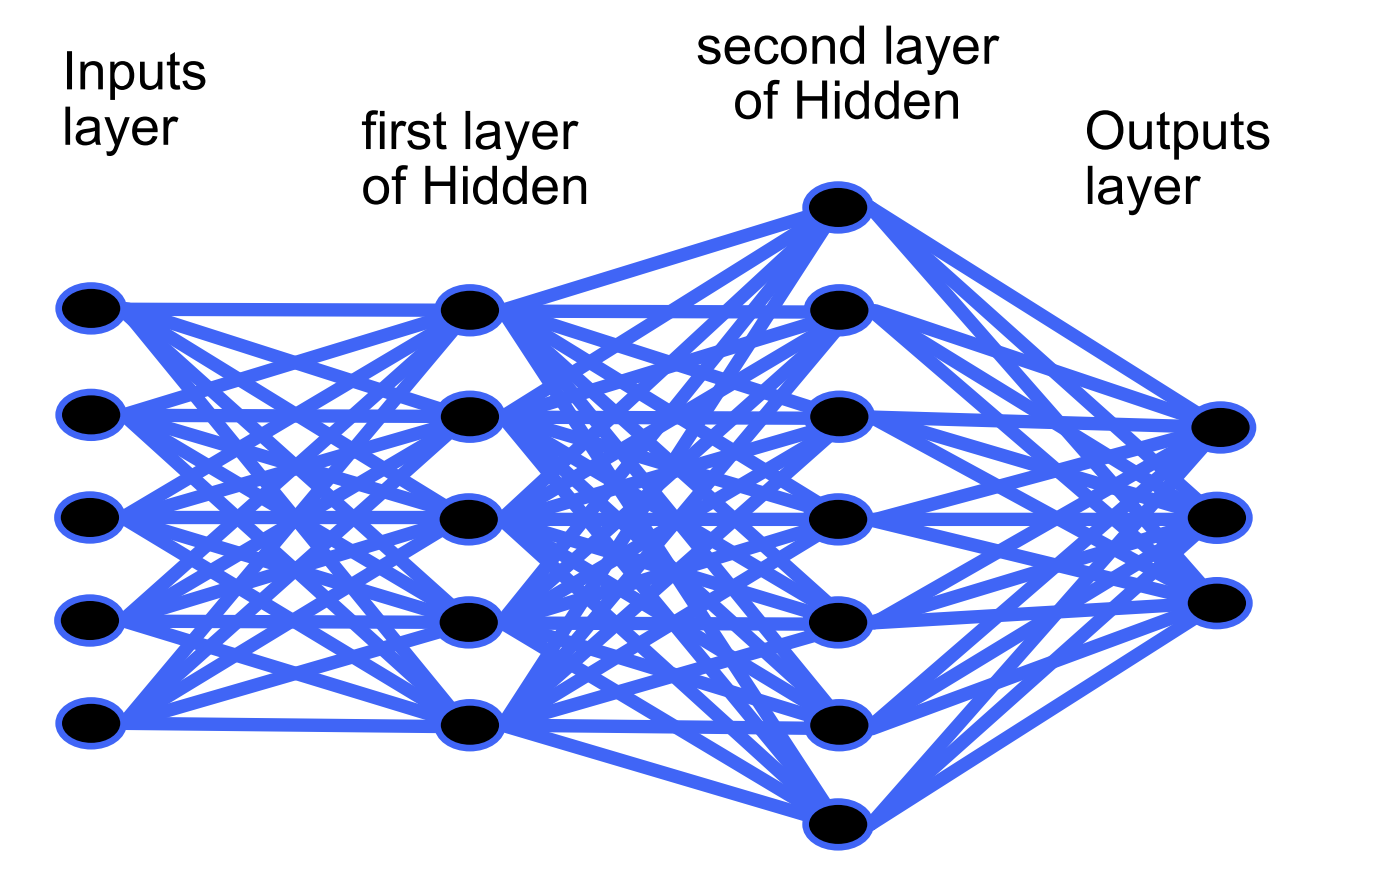
\includegraphics[width=0.5\textwidth]{images/nn.png}
    \captionsource{Ilustrasi Jaringan Saraf Tiruan pada Deep Learning}{\cite{cholissodin2020ai}}
    \label{fig:nn_deeplearning}
\end{figure}


\subsection{\textit{Convolutional Neural Networks} (CNN)}
\textit{Convolutional Neural Networks} (CNN) merupakan arsitektur jaringan saraf tiruan yang dirancang khusus untuk memproses data visual. CNN bekerja dengan mengidentifikasi pola atau fitur dalam gambar melalui operasi konvolusi yang diikuti oleh proses \textit{pooling}. Arsitektur ini menjadi dasar bagi berbagai metode modern dalam tugas-tugas pengenalan citra, deteksi objek, dan estimasi pose manusia.

Salah satu arsitektur CNN yang populer adalah AlexNet. AlexNet diperkenalkan oleh Krizhevsky et al. pada tahun 2012 dan menjadi tonggak penting dalam perkembangan \textit{deep learning} untuk tugas pengenalan citra. Arsitektur ini terdiri dari delapan lapisan, dengan lima lapisan konvolusional diikuti oleh tiga lapisan \textit{fully connected} (FC). AlexNet menggunakan fungsi aktivasi ReLU untuk mempercepat konvergensi pelatihan, serta teknik \textit{dropout} untuk mencegah \textit{overfitting}. Selain itu, AlexNet memperkenalkan penggunaan GPU dalam pelatihan jaringan, yang secara signifikan mempercepat proses komputasi \cite{NIPS2012_c399862d}. 

Keberhasilan AlexNet dalam memenangkan kompetisi \textit{ImageNet Large Scale Visual Recognition Challenge} (ILSVRC) pada tahun 2012 dengan peningkatan akurasi yang signifikan dibandingkan metode sebelumnya menjadikannya model yang mendasari pengembangan arsitektur CNN modern.


\begin{figure}[h!]
    \centering
    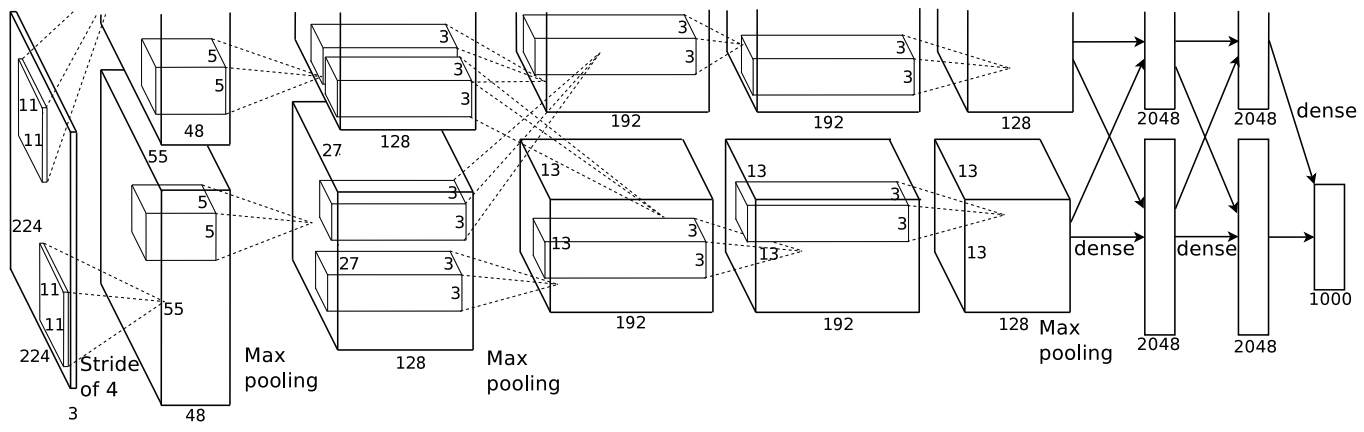
\includegraphics[width=0.9\textwidth]{images/alexnet_architecture.png}
    \captionsource{Arsitektur AlexNet}{\cite{NIPS2012_c399862d}}
    \label{fig:alexnet_architecture}
\end{figure}

\begin{figure}[h!]
    \centering
    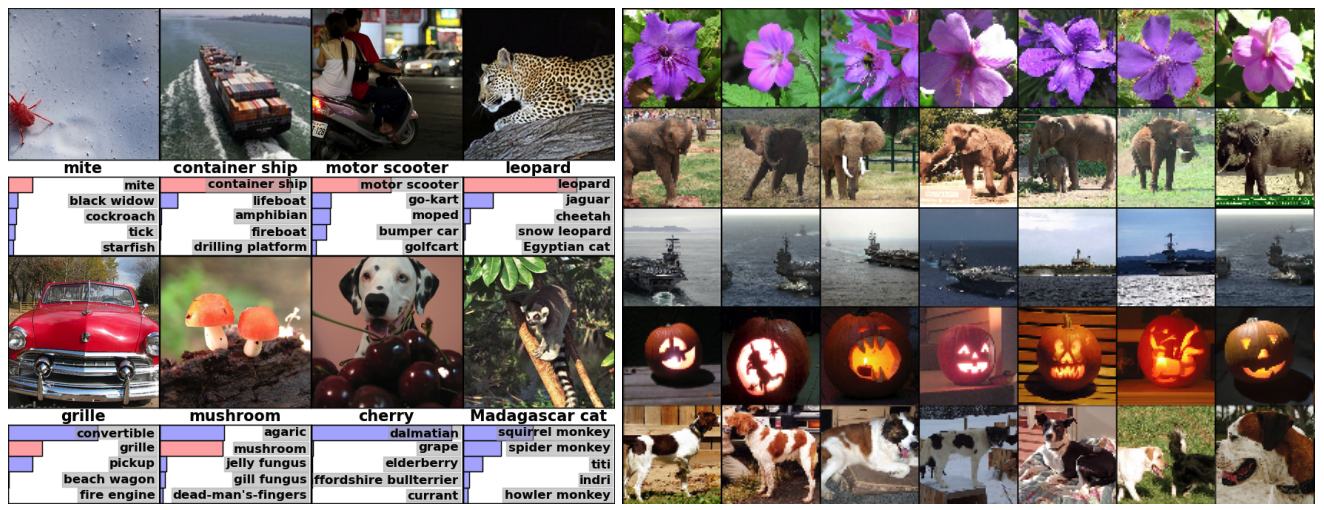
\includegraphics[width=0.9\textwidth]{images/alexnet_result.png}
    \captionsource{Hasil ILSVRC-2010 AlexNet}{\cite{NIPS2012_c399862d}}
    \label{fig:alexnet_result}
\end{figure}

\subsection{\textit{Transformer}}
\textit{Transformer} adalah arsitektur berbasis \textit{attention} yang pertama kali diperkenalkan oleh Vaswani et al. dalam makalah \textit{"Attention Is All You Need"}. Transformers dirancang untuk menggantikan arsitektur tradisional berbasis \textit{recurrent neural networks (RNN)} dan \textit{convolutional neural networks (CNN)} dalam berbagai tugas, khususnya dalam pemrosesan bahasa alami (\textit{natural language processing}, NLP). Keunggulan utama Transformers terletak pada mekanisme \textit{self-attention}, yang memungkinkan model untuk mempelajari hubungan antar elemen dalam data tanpa memerlukan pemrosesan berurutan, seperti pada RNN.

Dalam mekanisme \textit{self-attention}, setiap elemen input dibandingkan dengan elemen lainnya untuk menentukan relevansi antar elemen. Mekanisme ini direpresentasikan dalam bentuk \textit{query}, \textit{key}, dan \textit{value}, di mana relevansi dihitung sebagai nilai dot-product antara \textit{query} dan \textit{key}, yang kemudian digunakan untuk memberikan bobot pada elemen \textit{value} \cite{vaswani2017attention}. Pendekatan ini memungkinkan model untuk memahami hubungan jangka panjang (\textit{long-range dependencies}) dalam data, sehingga cocok untuk data berurutan seperti teks atau video.

\subsection{\textit{Pose Estimation}}
\textit{Pose estimation} adalah proses untuk menentukan lokasi spasial (\textit{keypoints}) tubuh manusia atau objek dalam representasi 2D atau 3D. Proses ini bertujuan untuk mendeteksi titik-titik penting, seperti kepala, siku, lutut, dan pergelangan tangan, yang membentuk kerangka tubuh manusia atau objek. Pada pendekatan modern, jaringan saraf konvolusional (\textit{Convolutional Neural Network}, CNN) digunakan untuk menghasilkan peta panas (\textit{heatmap}) 2D dari input berupa gambar atau video. \textit{Heatmap} ini merepresentasikan probabilitas keberadaan \textit{keypoints} pada setiap piksel gambar \cite{mehta2017vnect}. Untuk menghasilkan pose dalam ruang 3D, peta panas 2D digabungkan dengan informasi tambahan, seperti data kedalaman (\textit{depth}) dari sensor atau rekonstruksi spasial menggunakan teknik regresi koordinat 3D. Pendekatan ini memungkinkan prediksi posisi \textit{keypoints} secara akurat meskipun pada pose yang kompleks atau dalam lingkungan dengan sudut pandang kamera yang tidak ideal.

Saat ini, \textit{pose estimation} telah menjadi salah satu bidang utama dalam visi komputer, dengan berbagai aplikasi mulai dari animasi karakter, pengenalan gerakan manusia, hingga kontrol robot humanoid. Metode berbasis CNN, seperti OpenPose dan HRNet, telah menjadi standar untuk estimasi pose 2D dan 3D dengan akurasi tinggi. Selain itu, arsitektur modern seperti \textit{Transformers} telah diperkenalkan dalam \textit{pose estimation}, misalnya pada model VitPose. Pendekatan berbasis \textit{Transformers} ini menggunakan mekanisme \textit{self-attention} untuk menangkap hubungan spasial dan temporal antara \textit{keypoints}, sehingga menghasilkan prediksi pose 3D yang lebih stabil dan akurat, terutama untuk data video \shortcite{xu2022vitpose}. Keunggulan \textit{Transformers} terletak pada kemampuannya untuk mempelajari konteks yang lebih luas dari data visual, membuatnya ideal untuk tugas yang memerlukan pemahaman gerakan berurutan, seperti dalam penelitian ini yang berfokus pada gerakan tari tradisional Indonesia.

\subsection{MeTRAbs}
MeTRAbs (\textit{Metric-Scale Truncation-Robust Heatmaps for Absolute 3D Human Pose Estimation}) adalah metode yang digunakan untuk memperkirakan pose 3D manusia secara langsung dari gambar RGB, bahkan ketika sebagian tubuh tidak terlihat sepenuhnya dalam gambar. Berbeda dengan metode sebelumnya yang hanya bisa memperkirakan posisi relatif antar sendi tubuh, MeTRAbs mampu memprediksi posisi setiap sendi dalam satuan meter bukan hanya piksel pada gambar.

Metode ini menggunakan representasi \textit{heatmap} 3D, yaitu peta probabilitas untuk setiap titik sendi, yang dibuat dalam ruang tiga dimensi. Semua sumbu dari \textit{heatmap} ini menggunakan skala metrik (meter), bukan piksel, sehingga hasilnya lebih realistis. Jaringan yang digunakan dalam MeTRAbs adalah jaringan konvolusional yang umum digunakan pada visi komputer, seperti ResNet-50, tanpa bagian tambahan yang rumit.

Selain memprediksi posisi 3D relatif antar sendi, MeTRAbs juga dapat memperkirakan posisi absolut tubuh manusia dalam ruang kamera. Ini dilakukan dengan cara menggabungkan prediksi posisi 3D dengan prediksi posisi 2D pada gambar, lalu menghitung posisi tubuh secara keseluruhan menggunakan rumus dari model kamera. Proses ini dilakukan secara otomatis dalam jaringan, sehingga pelatihan bisa dilakukan secara menyeluruh dan efisien.


\begin{figure}[h!]
    \centering
    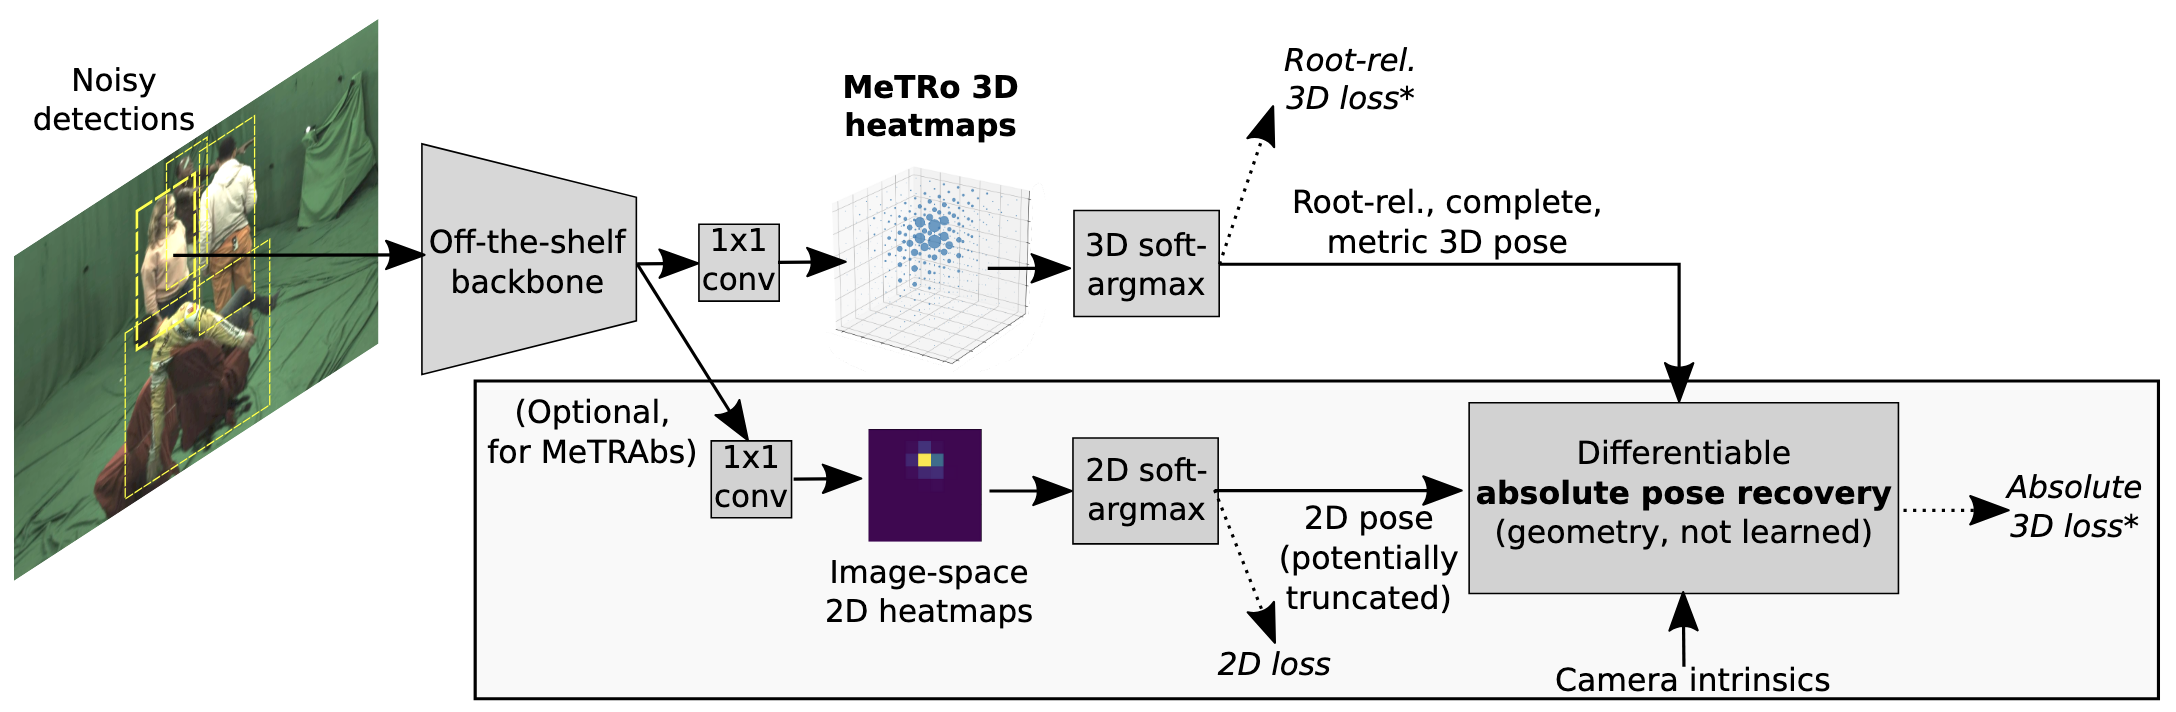
\includegraphics[width=\textwidth]{images/metrabs_architecture.png}
    \captionsource{Arsitektur jaringan MeTRAbs}{\cite{Sarandi2021metrabs}}
    \label{fig:metrabs_architecture}
\end{figure}

Keunggulan MeTRAbs adalah kemampuannya untuk tetap memberikan hasil estimasi yang baik meskipun gambar hanya menampilkan sebagian tubuh saja seperti pada Gambar~\ref{fig:metrabs_architecture}. Selain itu, metode ini tidak memerlukan informasi tambahan seperti panjang tulang atau jarak ke kamera saat pengujian.

\begin{figure}[h!]
    \centering
    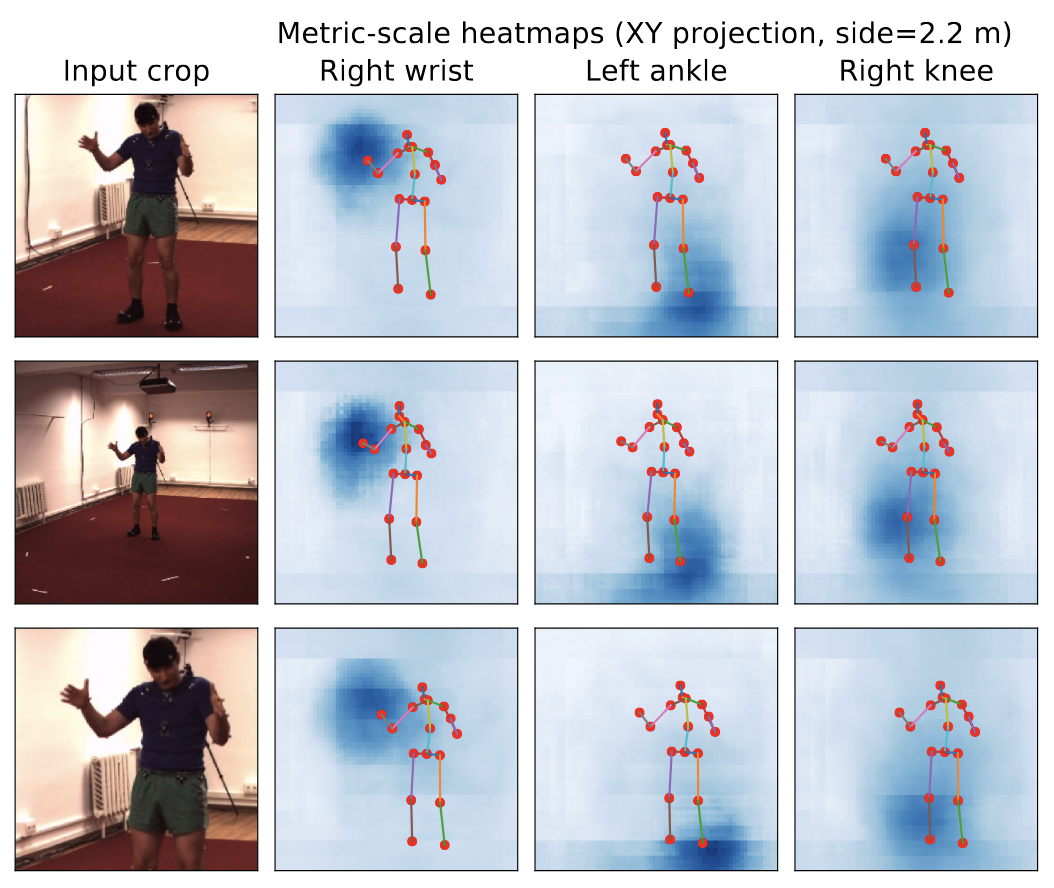
\includegraphics[width=0.6\textwidth]{images/metrabs_result.png}
    \captionsource{Keunggulan MeTRAbs}{\cite{Sarandi2021metrabs}}
    \label{fig:metrabs_result}
\end{figure}

\subsection{DeciWatch}

DeciWatch adalah sebuah kerangka kerja efisien yang dikembangkan untuk meningkatkan estimasi pose manusia 2D/3D pada video dengan mengurangi kebutuhan komputasi hingga 10 kali lipat tanpa mengorbankan akurasi~\cite{zeng2022deciwatch}. Alih-alih memproses setiap frame dalam video, DeciWatch hanya mengambil sebagian kecil frame (sekitar 10\%) melalui \textit{uniform sampling}. 

Arsitektur DeciWatch terdiri dari tiga tahap utama, yaitu \textit{sample-denoise-recover}. Pada tahap pertama, beberapa frame video dipilih secara merata. Pose pada frame-frame ini kemudian diperkirakan menggunakan pose estimator yang ada. Namun karena prediksi ini biasanya mengandung \textit{noise}, DeciWatch menggunakan DenoiseNet, sebuah jaringan berbasis \textit{transformer}, untuk membersihkan hasil estimasi dari noise.

Setelah itu, tahap ketiga dilakukan oleh RecoverNet, jaringan \textit{transformer} lain yang bertugas untuk merekonstruksi pose untuk frame-frame yang tidak diamati. RecoverNet memanfaatkan kontinuitas gerakan manusia dalam video untuk memperkirakan pose pada frame yang tidak diproses langsung. Pendekatan ini terbukti efektif dalam menghasilkan estimasi pose yang lebih halus dan konsisten, terutama pada gerakan yang cepat atau kompleks.

Keunggulan utama DeciWatch adalah efisiensinya. Karena hanya sebagian kecil frame yang dianalisis secara penuh, proses inferensi menjadi jauh lebih ringan, dengan konsumsi memori dan waktu komputasi yang lebih rendah. Selain itu, pendekatan ini juga memperhalus hasil estimasi pose karena mengurangi jitter atau getaran antar frame, menjadikannya sangat cocok untuk aplikasi video seperti pelacakan gerak, interaksi manusia-robot, dan pemodelan tari.

Eksperimen yang dilakukan pada berbagai \textit{dataset} termasuk AIST++ menunjukkan bahwa DeciWatch tidak hanya unggul dalam efisiensi, tetapi juga mampu meningkatkan akurasi secara signifikan dibandingkan metode estimasi frame-by-frame. Kemampuannya dalam menangani gerakan cepat dan data dengan noise menjadikannya sangat relevan dalam konteks penelitian ini.

\begin{figure}[H]
    \centering
    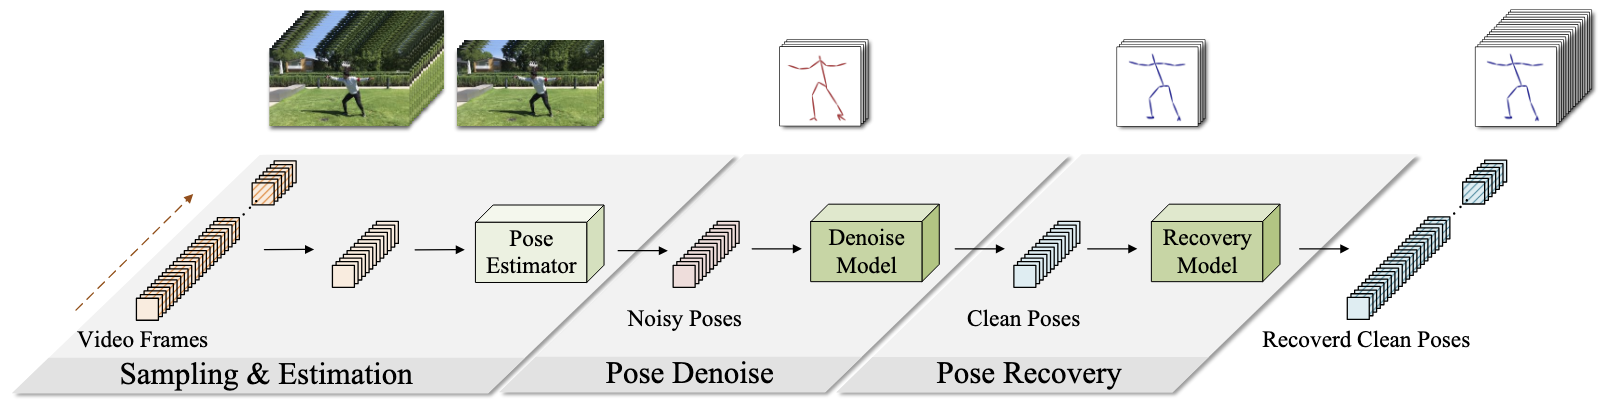
\includegraphics[width=\textwidth]{images/deciwatch_architecture.png}
    \captionsource{Arsitektur DeciWatch}{\cite{zeng2022deciwatch}}
    \label{fig:deciwatch_architecture}
\end{figure}

\subsection{Trigonometri}

Trigonometri adalah cabang matematika yang mempelajari hubungan antara sudut dan panjang sisi dalam segitiga \shortcite{trigono2008maharaj}. Dalam konteks robotika, khususnya pada perhitungan \textit{inverse kinematics}, trigonometri digunakan untuk menentukan sudut artikulasi berdasarkan posisi kartesian dari titik-titik tertentu pada tubuh robot atau manusia. Konsep dasar trigonometri berpusat pada perbandingan sisi dalam segitiga siku-siku, seperti berikut:

\begin{equation}
\sin \theta = \frac{\text{depan}}{\text{miring}}, \quad
\cos \theta = \frac{\text{samping}}{\text{miring}}, \quad
\tan \theta = \frac{\text{depan}}{\text{samping}}
\end{equation}

Pada aplikasi perhitungan sudut dari vektor posisi, fungsi \textit{arctangent} sering digunakan untuk mengubah rasio sisi menjadi sudut. Fungsi ini merupakan kebalikan dari \textit{tangent}, yang mengembalikan nilai sudut \(\theta\) dari rasio \(\frac{y}{x}\). Secara umum, perhitungan sudut menggunakan \textit{arctangent} dapat dituliskan sebagai:

\begin{equation}
\theta = \arctan\left(\frac{y}{x}\right)
\end{equation}

Namun, penggunaan fungsi \(\arctan\) biasa memiliki keterbatasan karena tidak dapat membedakan kuadran dengan benar, sehingga rawan menghasilkan sudut yang salah jika tanda dari \(x\) atau \(y\) berbeda. Untuk mengatasi masalah ini, digunakan fungsi \(\arctan2\), yaitu fungsi khusus yang mempertimbangkan tanda dari \(x\) dan \(y\) secara langsung, sehingga dapat menentukan sudut dengan tepat pada semua kuadran. Notasi umumnya adalah:

\begin{equation}
\theta = \arctan2(y, x)
\end{equation}

Fungsi \(\arctan2\) menghasilkan sudut dalam satuan radian dengan rentang \(-\pi\) hingga \(\pi\), yang sesuai dengan rotasi penuh pada bidang kartesian. Hal ini sangat penting dalam aplikasi robotika untuk memastikan orientasi sudut sesuai dengan posisi aktual vektor di ruang dua dimensi maupun tiga dimensi. Penggunaan trigonometri seperti ini menjadi komponen utama dalam proses \textit{motion retargeting} pada sistem robot humanoid, karena memungkinkan konversi dari data posisi menjadi sudut artikulasi yang dapat dijalankan oleh robot.


\subsection{Matriks Rotasi}

Matriks rotasi adalah alat matematis yang digunakan untuk memutar vektor dalam ruang dua atau tiga dimensi~\shortcite{palazzolo1976rotation}. Dalam bidang robotika, matriks rotasi digunakan untuk mentransformasikan posisi dan orientasi dari satu sistem koordinat ke sistem lainnya, seperti dalam proses \textit{motion retargeting} atau \textit{inverse kinematics}. Rotasi dalam ruang tiga dimensi dapat dinyatakan dengan matriks $3\times3$ untuk masing-masing sumbu utama:

\begin{equation}
R_x(\theta) =
\begin{bmatrix}
1 & 0 & 0 \\
0 & \cos\theta & -\sin\theta \\
0 & \sin\theta & \cos\theta
\end{bmatrix}
\end{equation}

\begin{equation}
R_y(\theta) =
\begin{bmatrix}
\cos\theta & 0 & \sin\theta \\
0 & 1 & 0 \\
-\sin\theta & 0 & \cos\theta
\end{bmatrix}
\end{equation}

\begin{equation}
R_z(\theta) =
\begin{bmatrix}
\cos\theta & -\sin\theta & 0 \\
\sin\theta & \cos\theta & 0 \\
0 & 0 & 1
\end{bmatrix}
\end{equation}

Matriks ini sering digunakan secara berurutan untuk membentuk rotasi gabungan di ruang tiga dimensi sesuai urutan sumbu yang diinginkan. Dalam aplikasi robot humanoid, rotasi ini digunakan untuk mengubah orientasi lengan, kepala, atau bagian tubuh lain sesuai dengan data gerakan manusia.

\subsection{\textit{Inverse Kinematics Transform}}

\textit{Inverse Kinematics Transform} (IKT) adalah metode untuk menghitung sudut-sudut sendi robot berdasarkan posisi titik-titik tubuh manusia, seperti bahu, siku, dan pergelangan tangan, dengan memanfaatkan prinsip geometri dan trigonometri. Pada penelitian \textit{"Robust Regression-Based Motion Perception for Online Imitation on Humanoid Robot"} \shortcite{robust2017imitation}, IKT digunakan untuk mengontrol pergerakan lengan robot humanoid secara langsung dari data pose manusia.

Struktur lengan dianggap sebagai manipulator dua sendi (\textit{two-link manipulator}) dengan empat derajat kebebasan (DOF). Untuk menyederhanakan perhitungan dan mengurangi kompleksitas komputasi, digunakan metode solusi geometris yang bersifat hierarkis dan intuitif. Pendekatan ini lebih efisien dibandingkan metode aljabar karena menghindari solusi yang tidak unik serta mempercepat proses komputasi.

Sebagai contoh, perhitungan sudut pada lengan kiri dilakukan secara bertahap. Pertama, sudut \textit{shoulder pitch} ($\theta_{\text{Pitch}}$) dihitung dari perubahan posisi pada sumbu X dan Z:

\begin{equation}
\theta_{\text{Pitch}} = \arctan2(z_{\text{elbow}} - z_{\text{shoulder}}, x_{\text{elbow}} - x_{\text{shoulder}})
\end{equation}

Kemudian, sudut \textit{shoulder roll} ($\theta_{\text{Roll}}$) dihitung dari perubahan posisi pada sumbu Y terhadap proyeksi vektor lengan atas pada bidang XZ:

\begin{equation}
\theta_{\text{Roll}} = \arctan2(y_{\text{elbow}} - y_{\text{shoulder}}, \sqrt{(x_{\text{elbow}} - x_{\text{shoulder}})^2 + (z_{\text{elbow}} - z_{\text{shoulder}})^2})
\end{equation}

Setelah mendapatkan sudut bahu, vektor lengan bawah diproyeksikan ke sistem koordinat lokal dengan rotasi menggunakan matriks rotasi. Dari situ, sudut \textit{elbow yaw} dan \textit{elbow roll} dihitung dengan prinsip trigonometri serupa. Proses ini memastikan konversi posisi Cartesian menjadi sudut artikulasi dilakukan secara efisien dan dapat berjalan secara \textit{real-time}.

Metode IKT ini sangat sesuai untuk aplikasi \textit{motion retargeting}, karena memungkinkan robot humanoid untuk meniru gerakan manusia secara langsung tanpa proses optimisasi yang berat secara komputasi.


\subsection{\textit{Mean Per Joint Position Error} (MPJPE)}

\textit{Mean Per Joint Position Error} (MPJPE) adalah metrik evaluasi yang umum digunakan dalam estimasi pose manusia 3D. MPJPE mengukur rata-rata jarak Euclidean antara posisi hasil prediksi dan posisi \textit{ground-truth} dari setiap \textit{joint} tubuh manusia dalam ruang 3D. Dengan membandingkan posisi yang diprediksi dengan posisi sebenarnya, MPJPE memberikan gambaran seberapa akurat model memetakan pose manusia~\cite{WANG2021103225}.

Secara matematis, MPJPE dirumuskan sebagai berikut:
\begin{equation}
    E_{\text{MPJPE}}(f, \mathcal{S}) = \frac{1}{N_\mathcal{S}} \sum_{i=1}^{N_\mathcal{S}} \left\lVert P_{f, \mathcal{S}}^{(i)} - P_{gt, f, \mathcal{S}}^{(i)} \right\rVert_2
    \label{eq:mpjpe}
\end{equation}

Pada rumus di atas, \( f \) merepresentasikan satu frame video, dan \( \mathcal{S} \) adalah kerangka tubuh (\textit{skeleton}). \( P_{f, \mathcal{S}}^{(i)} \) merupakan vektor posisi 3D prediksi dari \textit{joint} ke-\( i \), sedangkan \( P_{gt, f, \mathcal{S}}^{(i)} \) adalah posisi 3D dari data \textit{ground-truth}. Nilai \( N_\mathcal{S} \) menyatakan jumlah total \textit{joints}, biasanya sebanyak 17.

Misalkan terdapat 3 titik sendi (\textit{joint}) dengan posisi prediksi dan \textit{ground-truth} berikut:

\begin{itemize}
    \item Joint 1: prediksi = (1, 2, 3), ground-truth = (1, 2, 2)
    \item Joint 2: prediksi = (2, 1, 0), ground-truth = (2, 2, 0)
    \item Joint 3: prediksi = (0, 0, 0), ground-truth = (1, 0, 0)
\end{itemize}

Jarak Euclidean untuk masing-masing joint:
\begin{align*}
    d_1 &= \sqrt{(1{-}1)^2 + (2{-}2)^2 + (3{-}2)^2} = \sqrt{1} = 1 \\
    d_2 &= \sqrt{(2{-}2)^2 + (1{-}2)^2 + (0{-}0)^2} = \sqrt{1} = 1 \\
    d_3 &= \sqrt{(0{-}1)^2 + (0{-}0)^2 + (0{-}0)^2} = \sqrt{1} = 1
\end{align*}

MPJPE = \( \frac{1 + 1 + 1}{3} = 1.0 \) satuan jarak (misal dalam milimeter).

Contoh ini menunjukkan bahwa jika rata-rata kesalahan jarak antara posisi yang diprediksi dan posisi sebenarnya adalah 1 mm, maka MPJPE-nya adalah 1 mm. Nilai MPJPE yang lebih kecil menandakan prediksi pose yang lebih akurat.








    \chapter{METODOLOGI PENENILITIAN}

\vspace{1em}
\section{Waktu dan Tempat Penelitian}

Peneliti akan melaksanakan penelitian ini di Laboratorium Robotika Politeknik Negeri Malang (Polinema). Pemilihan lokasi ini dilakukan karena fasilitas laboratorium yang memadai untuk penelitian robotika serta keterlibatan tim Kontes Robot Tari Indonesia (KRSTI) Polinema, yang relevan dengan topik penelitian ini. Rentang waktu penelitian direncanakan mulai dari bulan Januari 2025 hingga Mei 2025. Pengujian sistem dan implementasi akan dilakukan di Laboratorium Robotika Polinema dengan dukungan tim Polinema Robotics.

\section{Diagram Alir Penelitian}

Untuk membuat sistem gerak robot berdasarkan \textit{pose estimation}, dimulai dengan perancangan sistem kemudian diimplementasikan. Berikut ini pada~\ref{fig:flowchart_penelitian} merupakan diagram alir dari penelitian yang dilakukan.

\begin{figure}[H]
    \centering
    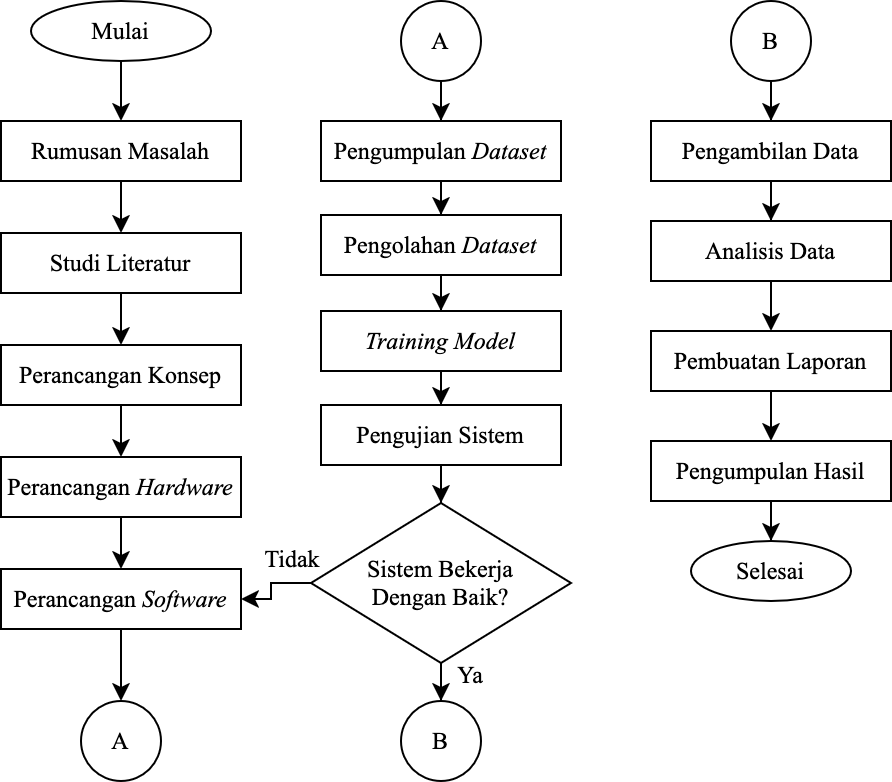
\includegraphics[width=0.9\textwidth]{images/flowchart_penelitian.png}
    \caption{Diagram Alir Penelitian}
    \label{fig:flowchart_penelitian}
\end{figure}

Penelitian ini dilaksanakan melalui serangkaian tahapan sistematis yang bertujuan untuk mengembangkan sistem pemodelan gerak tari tradisional Indonesia pada robot \textit{humanoid} berbasis estimasi pose 3D. Proses dimulai dengan perumusan masalah, yaitu mengidentifikasi tantangan utama dalam mengubah gerakan tari manusia menjadi representasi gerak yang dapat diimplementasikan pada robot. Setelah masalah dirumuskan, dilakukan studi literatur untuk memperoleh pemahaman yang mendalam mengenai teori dan teknologi yang mendasari, seperti metode \textit{pose estimation} (MeTRAbs, DeciWatch), pemrosesan dataset, dan pengendalian gerakan robot.
Penelitian ini dilakukan melalui serangkaian tahapan terstruktur yang bertujuan untuk menghasilkan sistem pemodelan gerak tari tradisional Indonesia pada robot \textit{humanoid} menggunakan metode estimasi pose. Alur penelitian diawali dengan identifikasi dan perumusan masalah, kemudian dilanjutkan dengan studi literatur untuk memperkuat dasar teori. Setelah itu dilakukan perancangan konsep dan perangkat lunak yang dibutuhkan, disusul oleh proses pengumpulan dan pengolahan data. 

Model dilatih menggunakan data yang telah disiapkan, kemudian diuji untuk menilai kinerjanya. Apabila hasil pengujian belum sesuai, dilakukan evaluasi dan perbaikan sistem. Jika sistem telah berfungsi dengan baik, proses dilanjutkan dengan pengambilan data hasil, analisis, penyusunan laporan, dan pengumpulan hasil akhir. 

\section{Metode Pengumpulan Data}

Pengumpulan data dilakukan untuk memperoleh informasi yang diperlukan dalam mendukung pelaksanaan penelitian, terutama terkait pengembangan dan pengujian sistem estimasi pose. Data yang digunakan dalam penelitian ini terdiri dari dua jenis utama, yaitu \textit{dataset} standar untuk pelatihan model dan data pengujian dari video tari tradisional Indonesia.

\subsection{\textit{Dataset} AIST++}

Penelitian ini menggunakan \textit{dataset} AIST++, yang merupakan salah satu \textit{benchmark dataset} standar untuk pelatihan dan evaluasi model estimasi pose manusia 3D, khususnya dalam konteks gerakan tari. \textit{AIST++} adalah \textit{dataset} yang dirancang untuk menangkap gerakan tari yang kompleks dan beragam, berisi lebih dari 10 juta frame video dengan anotasi pose 3D pada 60 fps~\shortcite{li2021ai}. \textit{Dataset} ini mencakup berbagai gaya tarian, seperti hip-hop, ballet, breakdance, jazz, dan gaya lainnya, yang memberikan keragaman gerakan tubuh secara spasial dan temporal, sehingga sangat cocok untuk melatih model yang fokus pada dinamika gerakan yang cepat dan bervariasi.

Dalam penelitian ini, digunakan dua jenis data dari \textit{dataset} AIST++ yakni hasil estimasi pose 3D dari video menggunakan model SPIN (\textit{SMPLify-X In the Loop}) dan data \textit{ground truth} pose 3D yang tersedia secara terbatas. Hal ini disebabkan oleh keterbatasan akses terhadap data video raw asli secara penuh, sehingga proses pelatihan model DeciWatch dilakukan menggunakan hasil prediksi SPIN sebagai data input dan data anotasi AIST++ sebagai target.

Data yang digunakan telah disusun dalam format .npz, yang berisi urutan pose 3D, parameter bentuk tubuh (shape), nama frame video, serta parameter kamera. Setiap file merepresentasikan satu sekuens gerakan dalam bentuk array dua dimensi, dengan jumlah frame yang bervariasi, rata-rata antara 300 hingga 600 frame per sekuens. Dataset ini dibagi menjadi dua bagian: data pelatihan (\textit{train}) sebanyak 7.292 sekuens dengan total 5.916.474 frame, dan data validasi (\textit{val}) sebanyak 3.840 sekuens dengan total 2.882.640 frame.

Penggunaan \textit{dataset} AIST++ dalam penelitian ini dimaksudkan untuk melatih dan mengevaluasi model DeciWatch agar mampu mengenali dan menyempurnakan estimasi pose manusia dalam konteks gerakan tari. Kompleksitas dan keragaman data AIST++ menjadikannya relevan untuk mengembangkan model yang nantinya diharapkan dapat diadaptasikan pada representasi gerakan tari tradisional Indonesia yang memiliki karakteristik gerak yang dinamis dan kompleks.


\begin{figure}[H]
    \centering
    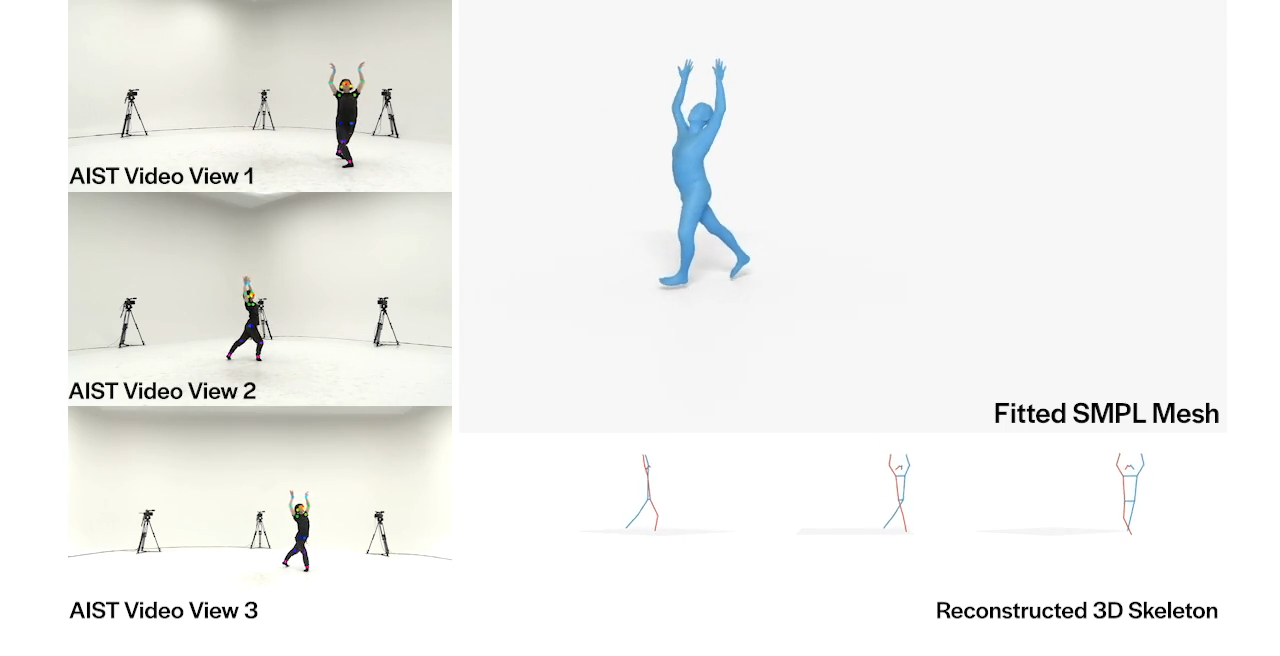
\includegraphics[width=0.7\textwidth]{images/aist.png}
    \captionsource{\textit{Dataset} AIST++}{\cite{li2021ai}}
    \label{fig:aist}
\end{figure}


\subsection{Data Video Tari Tradisional Indonesia}
Untuk pengujian model, data yang digunakan berasal dari video tari tradisional Indonesia yang diambil dari platform seperti YouTube. Video yang dipilih harus memenuhi beberapa kriteria, yaitu:
\begin{itemize}
    \item Menampilkan gerakan tari secara jelas dan berkelanjutan.
    \item Menggunakan teknik pengambilan gambar dengan kamera statis untuk meminimalkan gangguan visual.
    \item Memuat berbagai jenis tari tradisional Indonesia yang representatif.
\end{itemize}

Video-video ini kemudian diproses untuk menghasilkan \textit{keypoints} yang akan digunakan dalam evaluasi performa model estimasi pose. Sebagai contoh, gerakan tari seperti Denok Semarangan yang khas dan memiliki pola gerakan unik dapat menjadi bahan pengujian yang ideal untuk mengukur performa model.

\begin{figure}[H]
    \centering
    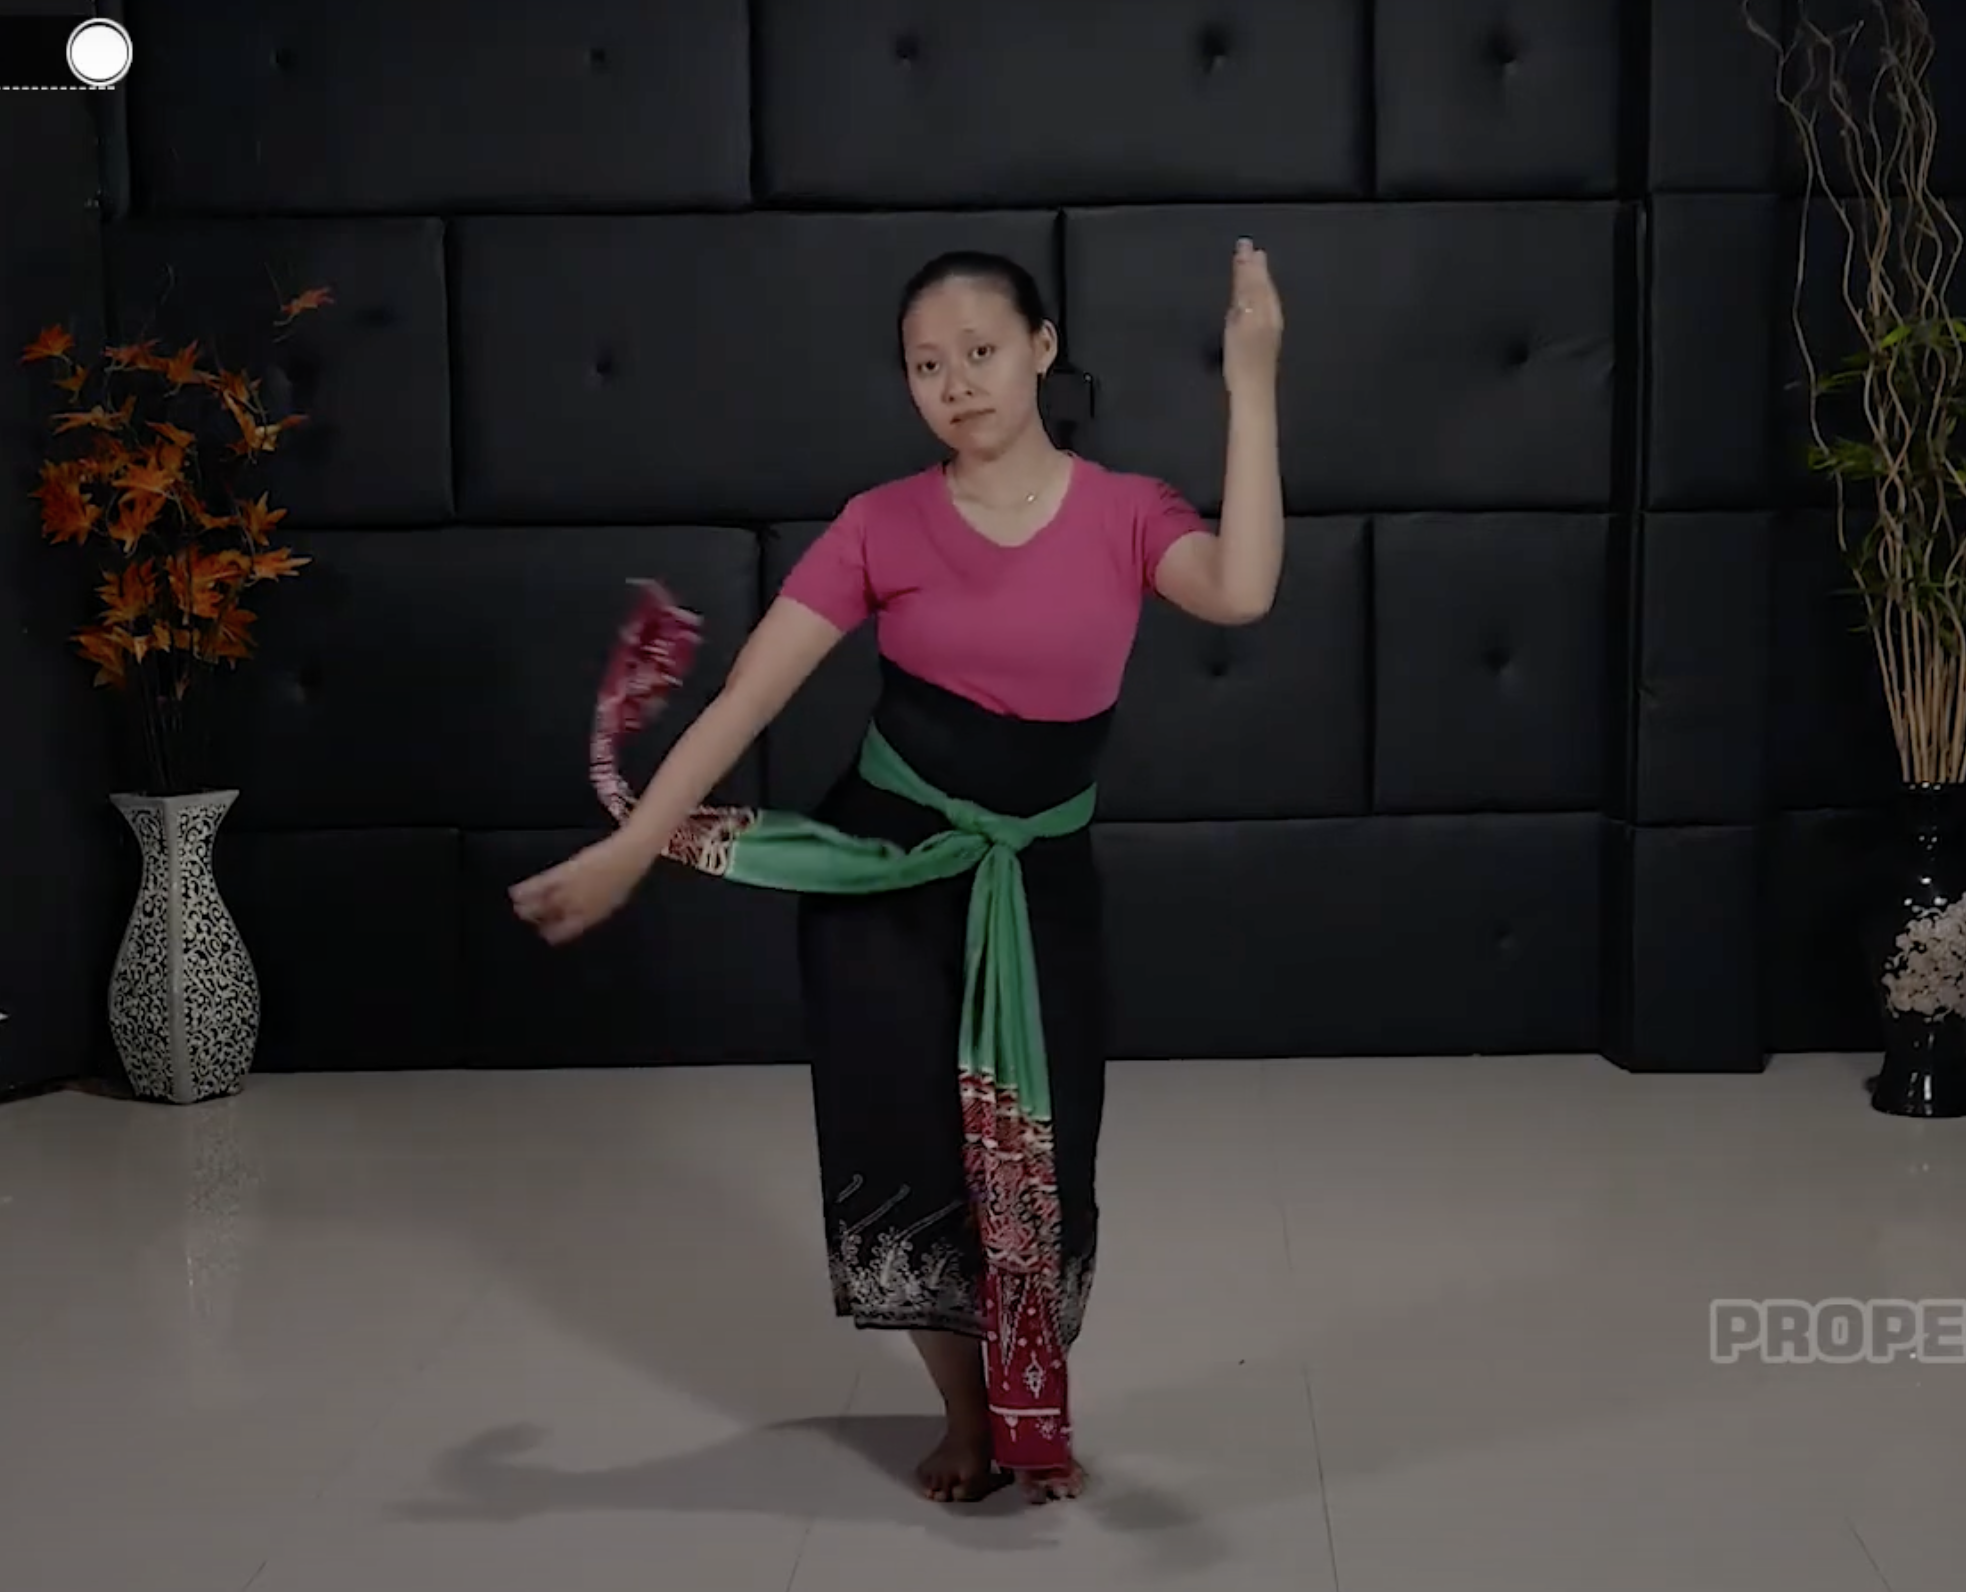
\includegraphics[width=0.5\textwidth]{images/dance_traditional.png}
    \captionsource{Tari Denok Semarangan}{YouTube}
    \label{fig:traditional_dance}
\end{figure}

\section{Teknik Pengolahan Data}

\begin{figure}[H]
    \centering
    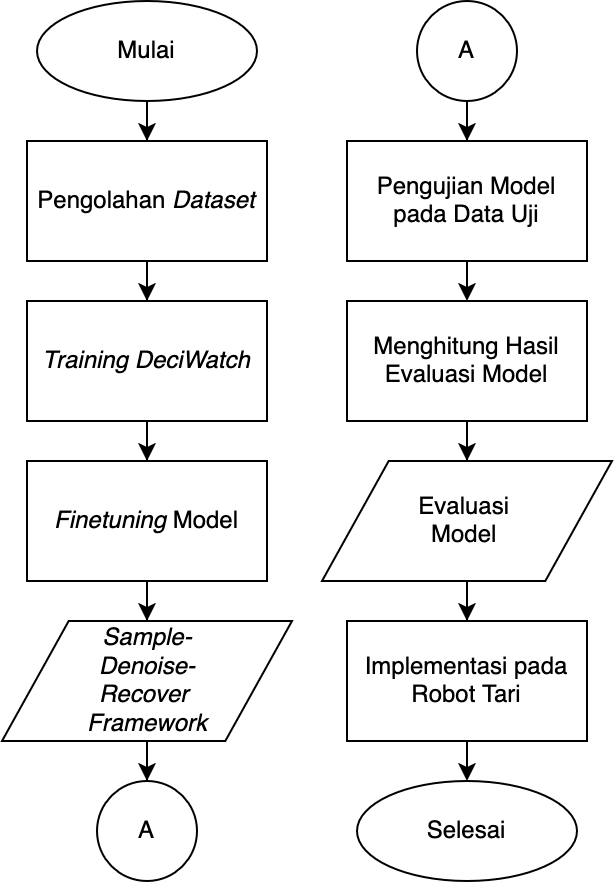
\includegraphics[width=0.5\textwidth]{images/flowchart_pengolahan.png}
    \caption{Diagram Alur Pengolahan Data}
    \label{fig:data_flowchart}
\end{figure}

\subsection{Pengolahan \textit{Dataset}}

Pada penelitian ini, \textit{dataset} yang digunakan berasal dari AIST++ Human Motion Dataset, yang sudah tersedia dalam bentuk data pose 3D yang siap digunakan tanpa perlu proses anotasi atau pengambilan data tambahan. Dataset ini telah diolah oleh pengembang DeciWatch dan dilengkapi dengan anotasi \textit{ground truth} serta hasil prediksi pose dari model SPIN. Struktur data AIST++ yang digunakan terdiri dari dua jenis data utama, yaitu:

\begin{itemize}
    \item \textit{Ground Truth Pose}: Berisi parameter koordinat 3D untuk 14 titik sendi tubuh.
    \item \textit{Predicted Pose (SPIN)}: Berisi hasil prediksi pose dari model SPIN yang berupa koordinat 3D titik sendi.
\end{itemize}

Adapun langkah-langkah pengolahan \textit{dataset} yang dilakukan dalam penelitian ini meliputi:

\begin{enumerate}
    \item {Pemilihan Data Latih dan Data Uji} \\
    Data dibagi menjadi dua bagian utama, yaitu data pelatihan (train) dan data pengujian (val). File {aist\_gt\_train.npz} dan {aist\_gt\_test.npz} digunakan untuk \textit{ground truth}, sedangkan {aist\_spin\_train.npz} dan {aist\_spin\_test.npz} digunakan untuk data prediksi SPIN.
    
    \item {Pemuatan dan Pemrosesan Struktur Data} \\
    Data dimuat menggunakan fungsi {numpy.load()} yang menghasilkan struktur dictionary berisi:
    \begin{itemize}
        \item {imgname}: Nama file dan indeks frame.
        \item {pose}: Parameter pose SMPL (72 dimensi).
        \item {trans}: Translasi gerakan 3D (3 dimensi).
        \item {scaling}: Faktor skala tubuh.
        \item {joints\_3d}: Koordinat 3D untuk 14 titik sendi utama.
    \end{itemize}
    
    \item {Pemetaan Keypoints} \\
    Data {joints\_3d} pada AIST++ memiliki urutan 14 titik sendi sesuai format: \textit{rankle, rknee, rhip, lhip, lknee, lankle, rwrist, relbow, rshoulder, lshoulder, lelbow, lwrist, neck, headtop}. Urutan ini identik dengan skema \textit{LSP-14} yang juga digunakan pada metode \textit{Metrabs}, sehingga kompatibel dengan standar pemetaan pose yang umum digunakan dalam literatur visi komputer. Pemetaan ini digunakan sebagai acuan dalam proses \textit{motion retargeting}, khususnya untuk menentukan titik-titik referensi pada perhitungan sudut sendi di robot humanoid.

    
    \item {Penyesuaian Input ke Model DeciWatch} \\
    Dataset ini kemudian digunakan sebagai input langsung ke model DeciWatch untuk proses prediksi pose berjangka waktu (temporal pose prediction). Karena DeciWatch membutuhkan input pose berurutan dalam bentuk sekuens, data pose diurutkan dan diproses dalam batch sesuai kebutuhan model.

\end{enumerate}

Proses ini tidak melibatkan anotasi manual karena seluruh data sudah tersedia dalam format yang sesuai untuk keperluan pelatihan dan pengujian model. Pengolahan dilakukan untuk memastikan data tersusun sesuai kebutuhan input pada sistem yang dikembangkan.


\subsection{\textit{Training} dan \textit{Fine-tuning} Model}
Setelah dataset hasil prediksi pose 3D oleh model Metrabs berhasil dikumpulkan dan diproses, langkah selanjutnya adalah melakukan pelatihan dan \textit{fine-tuning} model DeciWatch. Model ini bertujuan untuk meningkatkan akurasi estimasi pose secara temporal dengan memanfaatkan informasi antar-frame secara berurutan. 

Model DeciWatch dilatih menggunakan data input berupa pose 3D dari Metrabs sebagai \textit{frame-wise prediction}, kemudian disempurnakan melalui pembelajaran sekuensial untuk menghasilkan prediksi yang lebih halus dan akurat. Proses pelatihan dilakukan menggunakan \textit{framework} PyTorch dengan bantuan GPU yang mendukung CUDA dan cuDNN untuk mempercepat komputasi. Tahap \textit{fine-tuning} dilakukan dengan mengatur ulang parameter dan konfigurasi pelatihan agar model lebih sesuai dengan karakteristik data tari tradisional yang digunakan.


\subsection{Pengujian dan Evaluasi Model}

Model yang telah dilatih kemudian diuji menggunakan data uji yang berbeda dari data pelatihan untuk mengukur performanya. Evaluasi dilakukan dengan menghitung metrik \textit{Mean Per Joint Position Error} (MPJPE), yaitu rata-rata jarak Euclidean antara koordinat prediksi dan \textit{ground truth} dari setiap \textit{keypoint} dalam ruang 3D. Perhitungan MPJPE dilakukan sesuai dengan rumus yang telah dijelaskan pada Bab 2 pada persamaan (\ref{eq:mpjpe}). Nilai MPJPE yang lebih rendah menunjukkan akurasi prediksi yang lebih baik.

Proses evaluasi dilakukan dengan bantuan pustaka Python seperti NumPy untuk perhitungan matematis dan Matplotlib untuk analisis visualisasi hasil. Seluruh eksperimen dilakukan di lingkungan Jupyter Notebook atau Google Colab untuk mendukung fleksibilitas dalam pemrosesan dan pengujian model.




\subsection{Implementasi pada Robot Tari}
Setelah model dievaluasi, tahap berikutnya adalah implementasi pada robot humanoid ROBOTIS-OP3 untuk menguji kemampuan model dalam menghasilkan gerakan yang natural berdasarkan estimasi pose. Implementasi ini dilakukan dengan menggunakan bahasa pemrograman Python dan C++, serta memanfaatkan framework \textit{Robot Operating System} (ROS) untuk mengelola komunikasi antara perangkat keras dan perangkat lunak. Untuk menerjemahkan koordinat pose ke dalam pergerakan robot, digunakan konsep \textit{Inverse Kinematics} (IK) dengan dukungan pustaka Dynamixel SDK untuk mengontrol aktuator robot. Pengujian pergerakan robot juga dapat dilakukan di lingkungan simulasi menggunakan Gazebo dan Rviz sebelum diterapkan pada perangkat keras sebenarnya. 

% \section{Desain Sistem}
% \subsection{Diagram Blok Sistem}
% \begin{figure}[H]
%     \centering
%     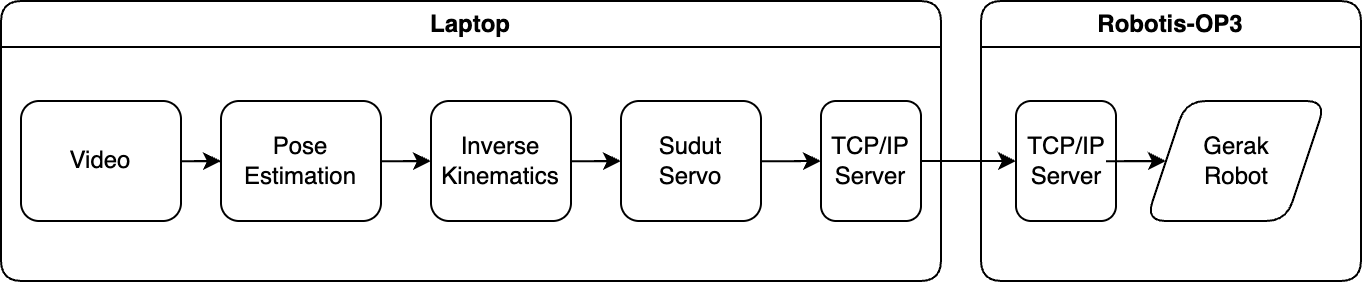
\includegraphics[width=0.8\textwidth]{images/sistem_diagram.png}
%     \caption{Diagram Sistem}
%     \label{fig:system_diagram}
% \end{figure}

% Seperti yang dapat dilihat pada Gambar \ref{fig:system_diagram}, input sistem berasal dari video yang memuat gerakan manusia. Data input ini kemudian diproses pada laptop menggunakan metode \textit{computer vision} dan \textit{deep learning} untuk melakukan estimasi pose tubuh manusia. Proses estimasi pose mendeteksi \textit{keypoints} tubuh, seperti kepala, tangan, dan kaki, yang kemudian dikonversi menjadi koordinat spasial. Selanjutnya, data pose ini diproses menggunakan metode \textit{inverse kinematics} untuk menghitung sudut-sudut sendi (\textit{servo angles}) yang sesuai. Data hasil perhitungan ini dikirimkan ke robot ROBOTIS-OP3 melalui protokol komunikasi TCP/IP bawaan ROS. Setelah diterima oleh robot, data sudut servo digunakan untuk menggerakkan robot, sehingga robot dapat mereplikasi gerakan yang ditampilkan dalam input. Output dari sistem adalah gerakan robot humanoid yang sesuai dengan data pose dari input video.

% \subsection{Flowchart Sistem}
% \vspace{1 em}
% \begin{figure}[H]
%     \centering
%     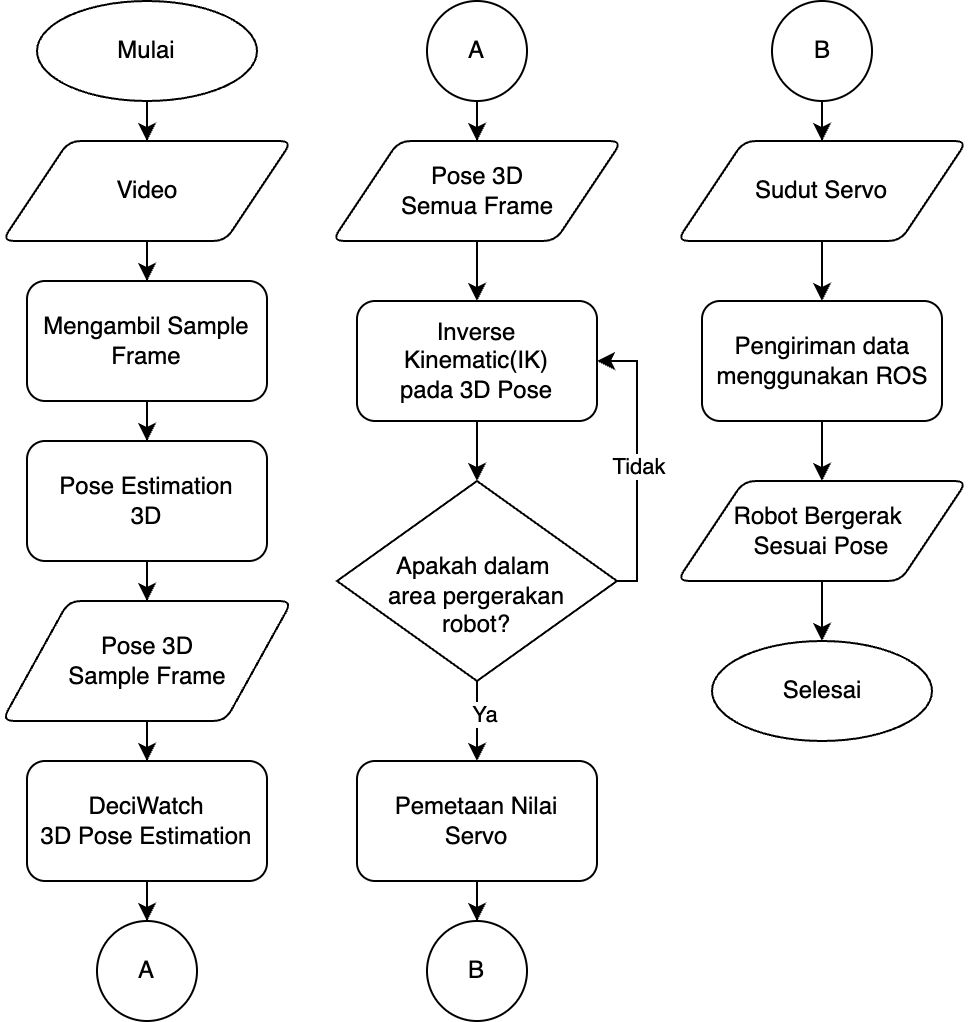
\includegraphics[width=0.7\textwidth]{images/flowchart.png}
%     \caption{Flowchart System}
%     \label{fig:system_flowchart}
% \end{figure}


% Flowchart pada Gambar \ref{fig:system_flowchart} menggambarkan alur proses estimasi pose 3D menggunakan metode DeciWatch serta implementasinya pada robot humanoid. Proses dimulai dengan input berupa video yang menjadi sumber data utama. Dari video ini, sampel frame diambil untuk mengurangi beban komputasi sekaligus memastikan kualitas data yang representatif untuk analisis pose.

% Setelah frame sampel diambil, pendapatan pose 3D awal dilakukan menggunakan model SPIN (\textit{SMPLify-X in the Loop}), yang merupakan salah satu metode estimasi pose 3D yang andal. SPIN menghasilkan pose 3D untuk setiap frame sampel, mencakup koordinat 3D dari titik-titik penting tubuh manusia. Data pose 3D awal ini kemudian diproses lebih lanjut menggunakan metode DeciWatch. DeciWatch memanfaatkan pendekatan \textit{sample-denoise-recover} untuk memperbaiki pose 3D dari frame yang telah dipilih, menghasilkan pose 3D yang lebih halus dan akurat dengan efisiensi komputasi yang tinggi.

% Pada bagian A, data pose 3D dari semua frame yang telah diproses menggunakan DeciWatch dilanjutkan dengan algoritma \textit{Inverse Kinematics} (IK). Algoritma IK bertugas untuk menghitung parameter gerakan robot berdasarkan pose 3D, serta memastikan apakah pose tersebut berada dalam area pergerakan robot. Jika pose tidak sesuai, proses kembali ke langkah IK untuk dilakukan penyesuaian. Namun, jika pose berada dalam area yang sesuai, data tersebut diteruskan ke proses pemetaan nilai servo.

% Bagian B mencakup pemetaan sudut servo berdasarkan data yang dihasilkan dari algoritma IK. Sudut servo yang telah dihitung kemudian dikirimkan ke robot menggunakan \textit{Robot Operating System} (ROS). Dengan ROS, data dikirimkan secara real-time untuk mengontrol pergerakan robot humanoid. Akhirnya, robot bergerak sesuai dengan pose yang telah dihitung, menghasilkan gerakan yang natural dan sesuai dengan data pose 3D awal.

% Flowchart ini mengintegrasikan berbagai komponen utama, seperti estimasi pose awal menggunakan SPIN, perbaikan pose menggunakan DeciWatch, algoritma IK, pemetaan servo, dan implementasi kontrol gerakan melalui ROS. Integrasi ini menghasilkan sistem yang efisien dan akurat untuk mengontrol gerakan robot berdasarkan data pose 3D.

\section{Uji Coba Sistem}

Uji coba sistem dilakukan untuk mengevaluasi keandalan dan kesesuaian fungsional sistem dalam mereplikasi gerakan manusia menggunakan robot humanoid ROBOTIS-OP3. Proses uji coba mencakup dua jenis pengujian utama, yaitu pengujian fungsional berupa \textit{black-box testing} dan pengujian performa dari model estimasi pose serta implementasi gerakan pada robot.

Secara umum, uji coba sistem difokuskan pada dua aspek utama berikut:

\begin{itemize}
    \item {Pengujian Fungsional Sistem (\textit{Black-Box Testing})}, yaitu pengujian terhadap alur kerja sistem secara keseluruhan, mulai dari input data gerak, pemrosesan melalui antarmuka berbasis \textit{website}, hingga eksekusi gerakan pada robot. Pengujian ini memastikan bahwa seluruh komponen sistem dapat berfungsi dengan baik tanpa melihat detail proses di dalamnya.
    
    \item {Pengujian Performa Estimasi dan Reproduksi Gerakan}, meliputi:
    \begin{itemize}
        \item \textit{Akurasi prediksi pose temporal} dari model DeciWatch, dengan evaluasi menggunakan metrik \textit{Mean Per Joint Position Error (MPJPE)} seperti pada persamaan (\ref{eq:mpjpe}).
        \item \textit{Kesesuaian hasil motion retargeting} pada robot ROBOTIS-OP3, yaitu evaluasi kualitas reproduksi gerakan robot terhadap urutan pose hasil prediksi serta kelancaran eksekusi pada saat proses \textit{playback}.
    \end{itemize}
\end{itemize}

Evaluasi ini dilakukan untuk memastikan sistem bekerja secara fungsional dan juga memiliki tingkat akurasi serta performa gerakan yang sesuai dengan kebutuhan pemodelan gerak tari tradisional Indonesia.



    \chapter{ANALISIS DAN PERANCANGAN SISTEM}
\vspace{1em}

\section{Deskripsi Sistem}
Sistem yang dikembangkan dalam penelitian ini merupakan sebuah aplikasi pemodelan gerak tari tradisional Indonesia dengan memanfaatkan teknologi \textit{pose estimation} dan robot \textit{humanoid} ROBOTIS-OP3. Sistem ini dirancang untuk mengekstraksi gerakan manusia dari video tari tradisional, menerjemahkannya ke dalam data koordinat 3D tubuh manusia, kemudian mengonversinya menjadi pergerakan fisik pada robot \textit{humanoid}.

Proses utama dari sistem dimulai dari input berupa video tari tradisional Indonesia yang dianalisis menggunakan model \textit{pose estimation} berbasis \textit{deep learning}. Model awal menggunakan pendekatan Metrabs (METa-learning TRAnsformer for 3D human pose eStimation) untuk menghasilkan koordinat pose 3D dari setiap frame dalam video, kemudian disempurnakan dengan metode DeciWatch yang meningkatkan akurasi dan kelancaran gerakan melalui pendekatan \textit{sample-denoise-recover}. Hasil estimasi berupa data \textit{keypoints} 3D kemudian dikonversi menjadi sudut-sudut servo (\textit{servo angles}) menggunakan algoritma \textit{Inverse Kinematics} (IK), dan seluruh data gerak tersebut disimpan dalam format file seperti JSON. File ini dapat digunakan untuk input kontrol robot \textit{humanoid} ROBOTIS-OP3 secara terpisah melalui sistem eksekusi gerak yang terintegrasi dengan ROS, sehingga memungkinkan robot untuk mereplikasi gerakan tari secara bertahap sesuai instruksi dalam file tersebut.

\section{Analisa Kebutuhan Sistem}

Dalam membangun sistem pemodelan gerak tari tradisional berbasis \textit{pose estimation}, dilakukan analisa kebutuhan terhadap perangkat keras (\textit{hardware}) dan perangkat lunak (\textit{software}) yang digunakan dalam proses pengolahan data, pelatihan model, serta integrasi dengan robot \textit{humanoid} ROBOTIS-OP3. Kebutuhan ini ditentukan berdasarkan tingkat kompleksitas komputasi dan kompatibilitas sistem.

\subsection{Kebutuhan Perangkat Keras}
Perangkat keras yang digunakan dalam penelitian ini terdiri dari laptop/PC untuk pengolahan data dan robot \textit{humanoid} ROBOTIS-OP3 sebagai platform eksekusi gerakan. Spesifikasi perangkat keras yang dibutuhkan adalah sebagai berikut:

\begin{longtable}{|c|p{9cm}|}
    \caption{Spesifikasi Perangkat Keras Laptop}
    \label{tab:spesifikasi_laptop} \\
    \hline
    \textbf{No} & \textbf{Nama Perangkat Keras} \\
    \hline
    \endfirsthead
    
    % \hline
    % \textbf{No} & \textbf{Nama Perangkat Keras} \\
    % \hline
    \endhead
    
    \hline
    \endfoot
    
    \hline
    \endlastfoot
    
    1 & Intel Core i5 Gen-10 \\ \hline
    2 & NVIDIA GeForce RTX 3060 6GB Mobile \\ \hline
    3 & RAM 16GB \\ \hline
    4 & SSD 256GB \\ \hline
    
\end{longtable}
    
\begin{longtable}{|c|p{9cm}|}
    \caption{Spesifikasi Perangkat Keras Robot}
    \label{tab:spesifikasi_robot} \\
    \hline
    \textbf{No} & \textbf{Nama Perangkat Keras} \\
    \hline
    \endfirsthead
    
    % \hline
    % \textbf{No} & \textbf{Nama Perangkat Keras} \\
    % \hline
    \endhead
    
    \hline
    \endfoot
    
    \hline
    \endlastfoot
    
    1 & Intel Core i3-7100U \\ \hline
    2 & RAM 8GB \\ \hline
    3 & SSD 256GB \\ \hline
    4 & Dynamixel XM430-W350, 2XL430-W250 \\ \hline
    
\end{longtable}
        
\subsection{Kebutuhan Perangkat Lunak}
Perangkat lunak yang digunakan dalam penelitian ini meliputi sistem operasi, bahasa pemrograman, dan berbagai pustaka (\textit{library}) yang mendukung pengolahan data, pelatihan model, serta komunikasi dengan robot. Berikut adalah spesifikasi perangkat lunak yang dibutuhkan:

\begin{longtable}{|c|p{5cm}|p{8cm}|}
    \caption{Spesifikasi Perangkat Lunak}
    \label{tab:kebutuhan_perangkat_lunak} \\
    \hline
    \textbf{No} & \textbf{Nama} & \textbf{Keterangan} \\
    \hline
    \endfirsthead
    
    % \hline
    % \textbf{No} & \textbf{Nama} & \textbf{Keterangan} \\
    % \hline
    \endhead
    
    \hline
    \endfoot
    
    \hline
    \endlastfoot
    
    1 & Sistem Operasi Laptop & Ubuntu 24.04 LTS \\ \hline
    2 & Sistem Operasi Robot & Linux Mint 16 \\ \hline
    3 & Bahasa Pemrograman & Python 3.9, C++, Bash \\ \hline
    4 & Text Editor & Visual Studio Code, Nano \\ \hline
    5 & Pustaka Pemrograman & TensorFlow, PyTorch, NumPy, OpenCV, Matplotlib, Flask \\ \hline
    6 & Robot Operating System & ROS Kinetic, ROS 2 Humble \\ \hline
    7 & Perangkat Lunak Pendukung & Jupyter Notebook, Google Colab \\ \hline
    
\end{longtable}
    

\subsection{Analisa Kebutuhan Fungsionalitas}

Analisis kebutuhan fungsional merupakan proses identifikasi dan dokumentasi terhadap fitur dan fungsi spesifik yang harus dimiliki oleh sistem. Proses ini bertujuan untuk mendefinisikan tugas-tugas utama yang dilakukan oleh sistem, cara sistem berinteraksi dengan pengguna, serta bagaimana sistem merespons input yang diterima. Kebutuhan ini menjadi dasar dalam proses perancangan dan implementasi sistem secara keseluruhan, sebagaimana ditunjukkan pada Tabel~\ref{tab:kebutuhan_fungsionalitas}.

\begin{longtable}{|c|p{5cm}|p{8cm}|}
\caption{Kebutuhan Fungsional Sistem}
\label{tab:kebutuhan_fungsionalitas} \\
\hline
\textbf{No} & \textbf{Fungsi} & \textbf{Deskripsi} \\
\hline
\endfirsthead

\hline
\textbf{No} & \textbf{Fungsi} & \textbf{Deskripsi} \\
\hline
\endhead

\hline
\endfoot

\hline
\endlastfoot

1 & Upload Video & Sistem menyediakan fitur bagi pengguna untuk mengunggah video tari tradisional Indonesia dalam format umum seperti MP4 atau AVI. Nama file akan tampil pada area log sebagai konfirmasi. \\
\hline
2 & Estimasi Pose dan Filtering & Sistem melakukan proses estimasi pose tubuh manusia dalam bentuk koordinat 3D \textit{keypoints} menggunakan model MeTRAbs dan DeciWatch. Hasil estimasi difilter untuk mengurangi noise pada prediksi temporal. \\
\hline
3 & Visualisasi Skeleton 3D & Sistem menampilkan hasil estimasi pose dalam bentuk skeleton 3D yang divisualisasikan sesuai urutan frame video. \\
\hline
4 & Status Log & Sistem mencatat dan menampilkan status proses seperti upload, estimasi, dan penyimpanan pada area log agar pengguna dapat memantau jalannya sistem. \\
\hline
5 & Penyimpanan Data & Sistem menyimpan hasil estimasi pose ke dalam file berformat JSON yang dapat digunakan untuk kontrol robot. File ini akan disimpan di direktori output. \\
\hline
6 & Playback Robot & Sistem mengontrol robot ROBOTIS-OP3 untuk mereproduksi gerakan berdasarkan file JSON hasil estimasi. Robot akan bergerak sesuai urutan sudut artikulasi yang dihasilkan dari \textit{motion retargeting}. \\
\hline

\end{longtable}


\section{Perancangan Sistem}

Perancangan sistem dilakukan untuk mendefinisikan bagaimana komponen-komponen dalam sistem saling berinteraksi dan berfungsi dalam keseluruhan proses pemodelan gerak tari tradisional menggunakan teknologi \textit{pose estimation}. Sistem ini dirancang dengan pendekatan modular, mulai dari tahap akuisisi video hingga penyimpanan data gerakan dalam format yang dapat dieksekusi oleh robot \textit{humanoid} ROBOTIS-OP3.

\subsection{Arsitektur Sistem}

\begin{figure}[H]
    \centering
    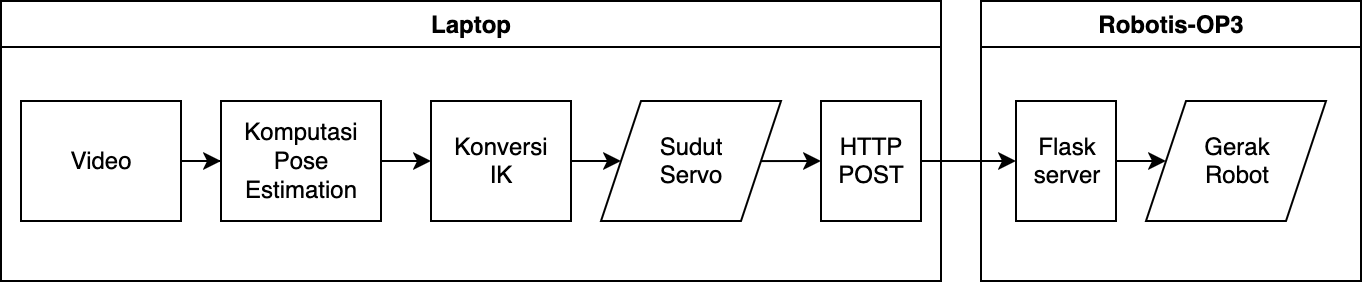
\includegraphics[width=0.9\textwidth]{images/arsitektur_sistem.png}
    \caption{Diagram Arsitektur Sistem}
    \label{fig:arsitektur_sistem}
\end{figure}

Gambar~\ref{fig:arsitektur_sistem} menunjukkan arsitektur sistem yang dikembangkan untuk pemodelan gerak tari tradisional menggunakan teknologi \textit{pose estimation}. Sistem ini terdiri dari dua bagian utama, yaitu pemrosesan data pada laptop dan eksekusi gerakan pada ROBOTIS-OP3.

Pada sisi laptop, input berupa video tari diproses melalui modul komputasi estimasi pose untuk memperoleh koordinat 3D tubuh manusia. Data koordinat ini kemudian dikonversi menggunakan algoritma \textit{Inverse Kinematics} (IK) menjadi sudut servo yang sesuai dengan struktur pergerakan robot. Sudut servo tersebut dikemas dalam format \textit{JSON} dan dikirimkan ke robot melalui protokol komunikasi \textit{HTTP POST} menggunakan \textit{Flask client} di sisi laptop.

Sementara itu, di sisi robot ROBOTIS-OP3, data gerakan diterima oleh \textit{Flask server}, kemudian disimpan dalam format file JSON sebagai rekaman gerak. Data ini digunakan untuk mengontrol aktuator robot sehingga menghasilkan gerakan yang sesuai dengan video input. Pendekatan ini memanfaatkan pemisahan beban komputasi, di mana proses komputasi berat dilakukan di laptop, sedangkan robot fokus pada eksekusi pergerakan. Metode ini juga memudahkan integrasi sistem dan pengujian karena menggunakan protokol \textit{HTTP} yang lebih sederhana dan fleksibel dibandingkan komunikasi \textit{socket}.



\subsection{Alur Kerja Sistem}

\begin{figure}[H]
    \centering
    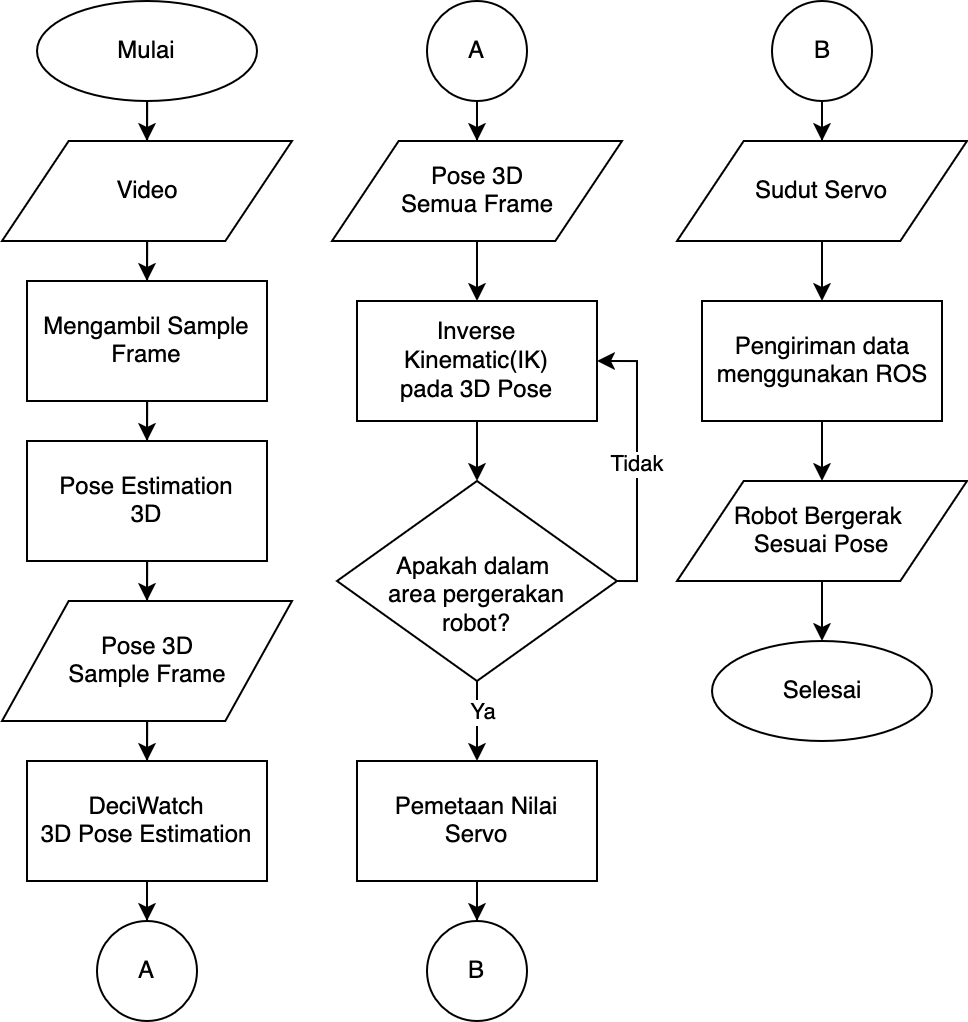
\includegraphics[width=0.8\textwidth]{images/system_flowchart.png}
    \caption{Flowchart Perancangan Sistem}
    \label{fig:flowchart_sistem}
\end{figure}

Gambar \ref{fig:flowchart_sistem} menunjukkan alur kerja sistem yang dirancang dalam penelitian ini, dimulai dari input video hingga eksekusi gerakan oleh robot \textit{humanoid} ROBOTIS-OP3. Berikut adalah penjelasan rinci tiap langkah dalam alur sistem:

\begin{enumerate}
    \item {Input Video} \\
    Sistem menerima masukan berupa video tari tradisional Indonesia dalam format umum seperti MP4.
    
    \item {Pengambilan Sampel Frame} \\
    Video diolah dengan mengambil sampel beberapa frame secara berkala untuk mengurangi beban komputasi dan menyesuaikan dengan kebutuhan input model.
    
    \item {Pose Estimation 3D} \\
    Setiap frame hasil sampel diproses menggunakan model \textit{pose estimation} berbasis Metrabs untuk menghasilkan prediksi koordinat 3D dari titik-titik persendian tubuh manusia. Sistem mendukung dua jenis model \textit{skeleton}, yaitu \textit{LSP-14} yang terdiri dari 14 titik persendian utama dan \textit{COCO-19} yang terdiri dari 19 titik, sehingga dapat disesuaikan dengan kebutuhan pemetaan gerakan pada robot.
    
    \item {DeciWatch 3D Pose Estimation} \\
    Output pose 3D dari Metrabs kemudian diolah lebih lanjut menggunakan DeciWatch. Model ini melakukan prediksi berurutan (temporal) untuk memastikan kontinuitas dan kelancaran gerakan antar-frame, sehingga menghasilkan estimasi pose 3D yang lebih halus.
    
    \item {Inverse Kinematics (IK) pada 3D Pose} \\
    Seluruh pose 3D hasil prediksi kemudian dikonversi menjadi sudut sendi menggunakan metode \textit{Inverse Kinematics Transform (IKT)}. Perhitungan ini dilakukan untuk mendapatkan sudut aktuator yang diperlukan agar robot dapat menirukan pose tersebut.
    
    \item {Validasi Area Pergerakan Robot} \\
    Sistem memeriksa apakah hasil perhitungan IK berada dalam jangkauan aktuator robot untuk menghindari servo bertabrakan. Jika tidak, maka pose akan disesuaikan agar tetap dalam batas gerak yang dapat dieksekusi oleh ROBOTIS-OP3 dengan cara membatasi sudut tersebut.
    
    \item {Pemetaan Nilai Servo} \\
    Setelah validasi, hasil IK dipetakan menjadi nilai sudut servo sesuai dengan konfigurasi servo pada robot.
    
    \item {Pengiriman Data ke Robot} \\
    Nilai sudut servo yang telah dihasilkan dari proses \textit{motion retargeting} dikirimkan ke robot menggunakan metode komunikasi berbasis HTTP POST. Data sudut servo dikemas dalam format \textit{JSON} dan dikirimkan melalui jaringan ke alamat IP robot.
    
    \item {Eksekusi Gerakan Robot} \\
    Robot ROBOTIS-OP3 akan mereplikasi gerakan sesuai dengan urutan pose yang telah dikirimkan, sehingga mampu merepresentasikan gerakan tari dalam bentuk fisik secara otomatis.
\end{enumerate}

Dengan alur ini, sistem secara menyeluruh dapat mengonversi gerakan manusia dari video menjadi pergerakan robot yang menyerupai gerakan asli secara berurutan dan sinkron.

\begin{lstlisting}[style=plainbox, caption={Pseudocode Struktur File JSON Gerakan}, label={lst:json_gerakan}]
{
  "frame_001": {
    "joint_1": 45.2,
    "joint_2": 30.8,
    ...
  },
  "frame_002": {
    "joint_1": 46.0,
    "joint_2": 32.1,
    ...
  },
  ...
}
\end{lstlisting}


Format ini memudahkan sistem kendali robot dalam membaca data per frame secara teratur dan menjalankan gerakan yang telah disesuaikan dengan hasil \textit{pose estimation}.

\section{Perancangan Antarmuka Pengguna}
    
\begin{figure}[H]
    \centering
    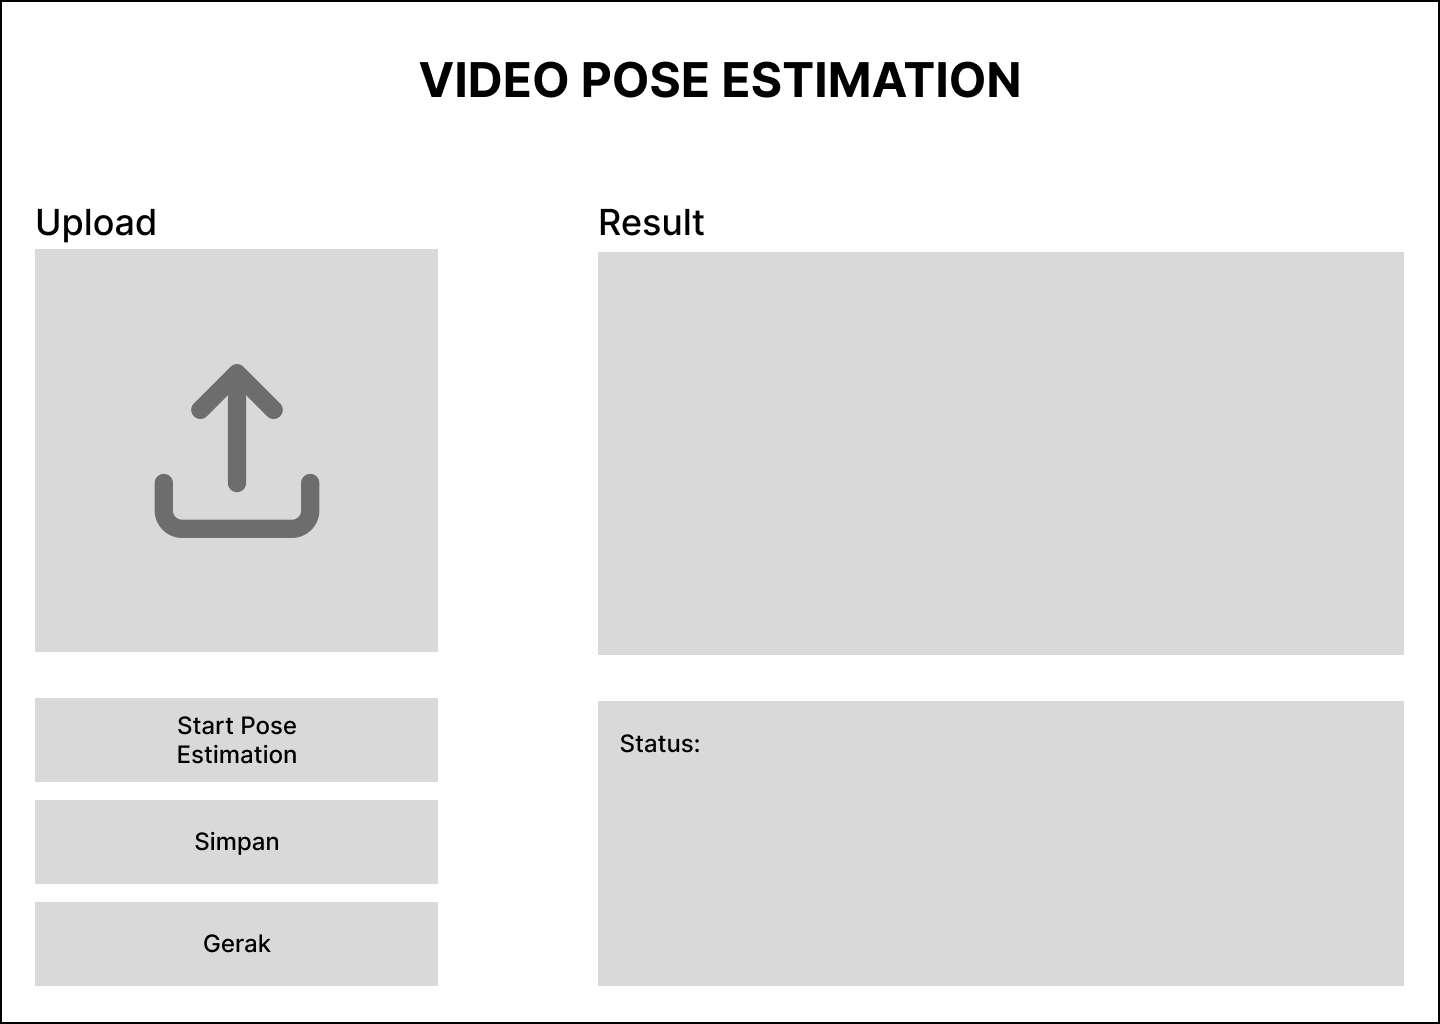
\includegraphics[width=0.8\textwidth]{images/Wireframe - 1.png}
    \caption{Perancangan Antarmuka Sistem}
    \label{fig:wireframe_ui}
\end{figure}

Gambar \ref{fig:wireframe_ui} menunjukkan rancangan awal antarmuka pengguna (UI) dari sistem yang dikembangkan. Antarmuka ini dirancang dengan tampilan yang sederhana dan intuitif untuk mendukung alur kerja mulai dari proses unggah video, estimasi pose 3D, hingga pengendalian gerak robot humanoid.

Di bagian kiri antarmuka terdapat elemen unggah video yang memungkinkan pengguna untuk memilih dan memasukkan video tari tradisional yang akan dianalisis. Setelah video berhasil diunggah, pengguna dapat memulai proses estimasi pose dengan menekan tombol "Start Pose Estimation". Proses ini akan mengaktifkan model \textit{pose estimation} untuk menghasilkan koordinat 3D dari setiap titik sendi tubuh manusia dalam video.

Hasil estimasi kemudian divisualisasikan pada area di sisi kanan antarmuka dalam bentuk tampilan \textit{3D skeleton}. Visualisasi ini memberikan gambaran postur dan gerakan tubuh dari objek dalam video secara menyeluruh berdasarkan estimasi pose yang telah dilakukan.

Setelah proses estimasi selesai, pengguna dapat menyimpan hasilnya dengan tombol "Simpan". Hasil yang disimpan berupa file JSON yang berisi informasi pose 3D dan sudut servo yang telah dihitung. Tombol "Gerak" digunakan untuk mengirimkan data gerak tersebut ke robot ROBOTIS-OP3 melalui sistem komunikasi ROS, sehingga robot dapat menirukan gerakan berdasarkan data yang telah diproses.

Di bagian bawah kanan antarmuka terdapat area status yang menampilkan informasi proses secara langsung, seperti log atau keluaran terminal. Area ini memberikan umpan balik kepada pengguna terkait status estimasi, penyimpanan data, maupun proses pengiriman ke robot, sehingga memudahkan dalam memantau dan mengontrol seluruh jalannya sistem.

\section{Perancangan Modifikasi Hardware}

Robot humanoid ROBOTIS-OP3 yang digunakan dalam penelitian ini merupakan platform robot terbuka yang dilengkapi dengan aktuator servo pada berbagai sendi tubuh. Namun, dalam bentuk standarnya, konfigurasi pergerakan tangan pada OP3 masih terbatas. Secara default, masing-masing lengan robot hanya memiliki tiga \textit{degree of freedom} (DoF), yaitu:
\begin{itemize}
    \item 2 DoF pada bahu (\textit{shoulder pitch} dan \textit{shoulder roll}),
    \item 1 DoF pada siku (\textit{elbow flexion}).
\end{itemize}

Konfigurasi ini cukup untuk gerakan dasar, namun belum mencukupi untuk mengekspresikan variasi gerakan tangan yang kompleks, seperti yang banyak ditemukan pada gerakan tari tradisional Indonesia yang menuntut rotasi pergelangan atau variasi gerak lengan secara lebih bebas.

Oleh karena itu, dilakukan modifikasi terhadap bagian tangan robot dengan menambahkan satu derajat kebebasan tambahan pada sendi siku berupa \textit{elbow twist}. Dengan penambahan ini, lengan robot memiliki total empat derajat kebebasan sebagai berikut:
\begin{itemize}
    \item 2 DoF pada bahu: \textit{pitch} dan \textit{roll},
    \item 2 DoF pada siku: \textit{flexion} dan \textit{twist}.
\end{itemize}

Penambahan DoF pada siku memungkinkan lengan robot untuk melakukan gerakan rotasi aksial, seperti memutar lengan bawah atau menyesuaikan arah tangan, yang sangat penting dalam meniru ekspresi gerak tangan pada tari tradisional. Modifikasi ini dilakukan dengan menambahkan satu motor servo tambahan yang dipasang secara koaksial pada sambungan siku, serta penyesuaian desain fisik dudukan servo agar tetap sesuai dengan struktur mekanik robot.

Modifikasi ini juga disertai dengan penyesuaian pada sistem kontrol dan inverse kinematics agar sistem dapat mengenali dan mengatur sudut baru tersebut. Dengan peningkatan fleksibilitas pada bagian lengan, robot memiliki kemampuan yang lebih tinggi dalam merepresentasikan gestur kompleks secara fisik dan artistik.



    \chapter{IMPLEMENTASI DAN PENGUJIAN}
\vspace{1em}
\section{Implementasi Sistem}
\subsection{Data \textit{Preprocessing}}
Pada tahap ini, proses \textit{data preprocessing} dilakukan untuk menyiapkan data pose 3D yang akan digunakan dalam pelatihan dan evaluasi model DeciWatch. Dataset yang digunakan merupakan dataset AIST++ yang menyediakan anotasi gerakan tari dalam format koordinat 3D, namun karena keterbatasan akses terhadap data video asli, proses deteksi pose awal dilakukan menggunakan model SPIN (\textit{SMPLify-X In the Loop}) yang memiliki struktur skeleton yang sama.

Model SPIN digunakan untuk mengekstraksi data pose 3D dari video tari yang tersedia dalam dataset AIST++. Hasil prediksi pose 3D dari SPIN kemudian dipasangkan dengan data \textit{ground truth} yang tersedia untuk keperluan pelatihan dan evaluasi model DeciWatch. Pasangan data ini terdiri dari dua bagian: data input berupa hasil estimasi pose dari SPIN, dan data target berupa anotasi pose 3D asli dari dataset AIST++ yang tersedia secara terbatas.

Setiap data pose 3D disimpan dalam format {.npz} yang berisi beberapa array utama. Struktur file {.npz} ini dijelaskan sebagai berikut:

Struktur data dalam file {.npz} yang digunakan pada sistem ini memiliki beberapa \textit{key} utama yang berisi informasi penting terkait pose 3D manusia untuk setiap sekuens gerakan. Setiap file menyimpan satu sekuens gerakan yang terdiri dari sejumlah frame, dengan format array sebagai berikut:

\begin{itemize}
    \item {\textit{imgname}} : Array berisi nama file atau jalur gambar dari frame-frame dalam sekuens. Tipe datanya adalah {numpy.ndarray} satu dimensi, dengan jumlah elemen sesuai panjang sekuens. Setiap elemen berupa string yang merepresentasikan nama atau jalur gambar dari masing-masing frame.
    
    \item {\textit{pose}} : Array dua dimensi dengan bentuk {(N, 72)}, di mana {N} adalah jumlah frame dalam sekuens. Setiap baris mewakili rotasi 24 sendi tubuh manusia dalam format axis-angle (masing-masing 3 dimensi, total 72). Data ini digunakan sebagai representasi postur tubuh untuk setiap frame.
    
    \item {\textit{shape}} : Array dua dimensi dengan bentuk {(N, 10)}, yang merepresentasikan parameter bentuk tubuh manusia dalam model SMPL. Nilai-nilai ini menggambarkan variasi bentuk tubuh dan tetap konstan sepanjang sekuens dalam kebanyakan kasus.
    
    \item {\textit{joints\_3d}} : Array dua dimensi dengan bentuk {(N, 3)}, yang menyimpan koordinat 3D dari titik pusat tubuh atau \textit{root joint} pada setiap frame. Koordinat ini digunakan sebagai referensi posisi global dalam ruang 3D.
    
    \item {\textit{camera}} : Array dua dimensi yang menyimpan parameter kamera per frame. Parameter ini digunakan dalam proses transformasi koordinat dari ruang kamera ke ruang dunia, serta untuk kebutuhan rendering ulang atau evaluasi terhadap data hasil prediksi.
\end{itemize}

Struktur ini berlaku untuk seluruh file {.npz} baik pada data pelatihan maupun validasi. Fleksibilitas format ini memungkinkan pemrosesan dan pelatihan model temporal seperti DeciWatch secara efisien dan modular berdasarkan sekuens per gerakan.

Dataset yang digunakan terdiri dari dua bagian utama, yaitu data pelatihan (\textit{train}) dan data validasi (\textit{val}). Pada bagian \textit{train}, terdapat sebanyak 7.292 sekuens gerakan dengan total 5.916.474 frame. Sementara itu, bagian \textit{val} terdiri dari 3.840 sekuens dengan total 2.882.640 frame. Rata-rata panjang setiap sekuens berkisar antara 300 hingga 600 frame, bergantung pada durasi dan kompleksitas gerakan dalam video.

Setiap sekuens menyimpan data dalam format {.npz}, yang berisi atribut seperti {pose}, {shape}, {joints\_3d}, dan {camera}. Struktur ini memungkinkan pengolahan data secara terpisah per sekuens, sekaligus memudahkan pelatihan model berbasis waktu seperti DeciWatch yang membutuhkan urutan frame yang berurutan dan konsisten. Dengan struktur yang terorganisir dan skala data yang besar, model dapat dilatih untuk mengenali pola gerakan manusia secara lebih akurat dan stabil dari waktu ke waktu.

Jumlah frame yang besar dan cakupan gerakan yang beragam dalam dataset ini memberikan fondasi yang kuat bagi model DeciWatch untuk belajar pola gerakan manusia secara kompleks dan merepresentasikannya secara halus dalam prediksi pose 3D.

\subsection{Inisialisasi Dataset dan \textit{DataLoader}}

Sebelum proses pelatihan dimulai, sistem terlebih dahulu memuat data pelatihan dan data uji dengan memanfaatkan kelas dataset yang telah disesuaikan dengan konfigurasi yang ditentukan. Proses ini dilakukan dengan memanggil fungsi \textit{dataset\_class} dan memberikan parameter seperti nama estimator (dalam hal ini menggunakan SPIN), jenis representasi tubuh (3D), serta bagian data yaitu \textit{train} atau \textit{test}. Pemanggilan ini akan menghasilkan dua objek yaitu \textit{train\_dataset} dan \textit{test\_dataset}.

Selanjutnya, kedua objek dataset tersebut dibungkus ke dalam \textit{DataLoader} dari PyTorch untuk memfasilitasi pemrosesan data dalam bentuk mini-batch selama proses pelatihan dan evaluasi model. Untuk data pelatihan digunakan ukuran batch sebesar 512 dan opsi \textit{shuffle} diaktifkan agar data tersaji secara acak pada setiap epoch. Sementara itu, pada data pengujian digunakan batch size 1 tanpa \textit{shuffle}, agar urutan data tetap terjaga selama proses evaluasi.

\begin{lstlisting}[style=plainbox, caption={Inisialisasi \textit{dataset} dan \textit{DataLoader} untuk pelatihan dan pengujian}, label={lst:dataloader}]
train_dataset = dataset_class(
                    dataset_name='aist',
                    estimator='spin',
                    return_type='3D',
                    sample_interval=5,
                    smpl_model_dir="data/smpl/",
                    phase='train'
                )

test_dataset = dataset_class(
                    dataset_name='aist',
                    estimator='spin',
                    return_type='3D',
                    sample_interval=5,
                    smpl_model_dir="data/smpl/",
                    phase='test'
                )

train_loader = DataLoader(
                    dataset=train_dataset,
                    batch_size=512,
                    shuffle=True,
                    num_workers=4,
                    pin_memory=True,
                    worker_init_fn=worker_init_fn
                )

test_loader = DataLoader(
                    dataset=test_dataset,
                    batch_size=1,
                    shuffle=False,
                    num_workers=4,
                    pin_memory=True,
                    worker_init_fn=worker_init_fn
                )

\end{lstlisting}

Penggunaan \textit{DataLoader} ini sangat penting untuk mengoptimalkan performa proses pelatihan model, terutama dalam hal efisiensi pemuatan data dari penyimpanan ke memori. Pengaturan seperti jumlah \textit{worker} dan aktivasi \textit{pin memory} membantu meningkatkan kecepatan transfer data antar proses dan perangkat GPU.


\subsection{Pembuatan Model}

Pada tahap ini dilakukan perancangan dan konfigurasi arsitektur model untuk menyempurnakan prediksi pose 3D secara temporal. Model yang digunakan adalah DeciWatch, yaitu model prediktif berbasis \textit{transformer encoder-decoder} yang dirancang untuk memproses urutan pose manusia dan menghasilkan prediksi yang lebih halus dan konsisten antar frame.

\begin{lstlisting}[style=plainbox, caption={Potongan isi file {config.yaml}}, captionpos=t, label={lst:config_yaml}]
MODEL:
    TYPE: network
    ENCODER_TRANSFORMER_BLOCK: 5
    ENCODER_EMBEDDING_DIMENSION: 128
    ENCODER_HEAD: 4
    ENCODER_RESIDUAL: true
    DECODER_TRANSFORMER_BLOCK: 6
    DECODER_EMBEDDING_DIMENSION: 128
    DECODER_HEAD: 4
    DECODER_RESIDUAL: true
    DECODER_TOKEN_WINDOW: 5
    SLIDE_WINDOW: true
    SLIDE_WINDOW_SIZE: 51
    SLIDE_WINDOW_Q: 10
\end{lstlisting}

Arsitektur model terdiri dari \textit{transformer encoder-decoder}, dengan konfigurasi sebagai berikut:

\begin{itemize}
    \item Encoder terdiri dari 5 blok transformer, dimensi embedding 128, 4 \textit{attention head}, dengan koneksi residual.
    \item Decoder terdiri dari 6 blok transformer, embedding 128, dengan token window berukuran 5.
    \item Pendekatan \textit{sliding window} digunakan untuk proses input sekuens dengan ukuran jendela 51 frame dan langkah pergeseran 10.
    \item Sampling frame dilakukan setiap 5 frame secara seragam.
\end{itemize}

Dataset yang digunakan adalah AIST++ dengan representasi tubuh 3D, menggunakan 14 titik sendi utama tanpa aktivasi SMPL.

Model diimplementasikan dengan PyTorch menggunakan kelas {DeciWatch} yang diturunkan dari {nn.Module}, seperti pada kode berikut:

\begin{lstlisting}[style=plainbox, caption={Model {DeciWatch}},captionpos=t, label={lst:deciwatch_model}]
model = DeciWatch(input_dim=train_dataset.input_dimension,
                  sample_interval=5,
                  encoder_hidden_dim=128,
                  decoder_hidden_dim=128,
                  dropout=0.1,
                  nheads=4,
                  dim_feedforward=256,
                  enc_layers=5,
                  dec_layers=6,
                  activation="leaky_relu",
                  pre_norm=True,
                  recovernet_interJ_method="linear",
                  recovernet_mode="transformer").to('cuda')
\end{lstlisting}


Inisialisasi ini memanfaatkan nilai \textit{input dimension} dari dataset pelatihan untuk menentukan jumlah fitur per frame yang akan diproses oleh model. Dengan parameter yang fleksibel dan bersifat modular, sistem ini memungkinkan penyesuaian cepat terhadap jenis data, panjang sekuens, atau kompleksitas gerakan yang berbeda pada skenario pelatihan lain di masa mendatang.

Setelah model berhasil diinisialisasi, langkah berikutnya adalah mendefinisikan fungsi loss dan algoritma optimisasi yang akan digunakan selama proses pelatihan. Pada sistem ini, digunakan kelas \textit{DeciWatchLoss} yang dirancang khusus untuk menghitung selisih antara hasil prediksi model dengan data \textit{ground truth} dalam bentuk pose 3D. Fungsi loss ini juga mendukung fitur tambahan seperti denoising dan regularisasi, yang dapat dikontrol melalui parameter konfigurasi.

Karena penelitian ini hanya difokuskan pada representasi pose dalam format 3D, maka fitur SMPL tidak diaktifkan (\textit{smpl = False}). Parameter seperti bobot loss untuk denoise (\textit{w\_denoise}) dan koefisien regularisasi (\textit{lamada}) diatur sesuai nilai pada file konfigurasi. Fungsi loss menggunakan kelas {DeciWatchLoss} dengan pengaturan:

\begin{itemize}
    \item Bobot denoise: 1.0
    \item Koefisien regularisasi (\(\lambda\)): 5.0
    \item SMPL: Tidak digunakan (hanya pose 3D)
\end{itemize}

\begin{lstlisting}[style=plainbox, caption={Inisialisasi fungsi loss dan optimizer}, label={lst:loss_optimizer}]
loss = DeciWatchLoss(w_denoise=1.0,
                     lamada=5.0,
                     smpl_model_dir="data/smpl/",
                     smpl=False)

optimizer = optim.Adam(model.parameters(), lr=0.001, amsgrad=True)
\end{lstlisting}

Setelah semua komponen siap, proses pelatihan dimulai dengan menggunakan kelas \textit{Trainer}. Kelas ini mengelola seluruh proses pelatihan dan pengujian model, termasuk perhitungan loss, evaluasi pada data validasi, logging, dan penyimpanan model. Metode {run()} dijalankan untuk memulai proses pelatihan berdasarkan konfigurasi yang telah ditentukan.

\begin{lstlisting}[style=plainbox, caption={Pemanggilan kelas Trainer untuk pelatihan model}, label={lst:trainer}]
Trainer(train_dataloader=train_loader,
        test_dataloader=test_loader,
        model=model,
        loss=loss,
        writer=writer,
        optimizer=optimizer,
        cfg=cfg).run()
\end{lstlisting}

% Untuk memperjelas konfigurasi pelatihan yang digunakan dalam penelitian ini, Tabel~\ref{tab:konfigurasi_pelatihan} menyajikan ringkasan parameter-parameter utama dalam proses pelatihan model DeciWatch. Tabel ini mencakup aspek arsitektur, optimisasi, serta pengaturan pelatihan yang relevan.


\begin{longtable}{|p{5cm}|p{8cm}|}
    \caption{Ringkasan Konfigurasi Pelatihan Model DeciWatch} \label{tab:konfigurasi_pelatihan} \\
    \hline
    \textbf{Komponen} & \textbf{Nilai} \\
    \hline
    \endfirsthead

    \hline
    \textbf{Komponen} & \textbf{Nilai} \\
    \hline
    \endhead

    Optimizer & Adam dengan AMSGrad \\
    \hline
    Learning rate & 0{,}001 \\
    \hline
    Jumlah epoch & 20 \\
    \hline
    Ukuran batch & 512 \\
    \hline
    Jumlah worker & 4 \\
    \hline
    Interval sampling & 5 frame \\
    \hline
    Dimensi embedding encoder & 128 \\
    \hline
    Jumlah blok encoder & 5 \\
    \hline
    Dimensi embedding decoder & 128 \\
    \hline
    Jumlah blok decoder & 6 \\
    \hline
    Dropout & 0{,}1 \\
    \hline
    Fungsi aktivasi & Leaky ReLU \\
    \hline
    Ukuran jendela (\textit{window size}) & 51 frame \\
    \hline
    Metode interpolasi temporal & Linear \\
    \hline
    Representasi tubuh & 3D (tanpa SMPL) \\
    \hline
\end{longtable}

Dengan struktur pelatihan ini, seluruh pipeline mulai dari pemuatan data, inisialisasi model, perhitungan loss, hingga pelatihan dan evaluasi dilakukan secara modular dan terintegrasi, sehingga memudahkan proses pengembangan serta eksperimen lanjutan.

\subsection{Metode Perhitungan MPJPE dan Prosedur Pelatihan Model}
\textit{Mean Per Joint Position Error} (MPJPE) merupakan metrik utama yang digunakan untuk mengevaluasi kualitas estimasi pose 3D. MPJPE menghitung jarak rata-rata antara posisi titik sendi hasil prediksi model dan \textit{ground truth} dalam ruang 3D. Semakin kecil nilai MPJPE, maka semakin akurat prediksi yang dihasilkan.

Perhitungan MPJPE dilakukan dengan menghitung \textit{euclidean distance} antara setiap titik prediksi dan \textit{ground truth} pada dimensi spasial (x, y, z), kemudian dirata-rata secara keseluruhan. Proses ini secara umum dituliskan sebagaimana pada rumus~\ref{eq:mpjpe}. Implementasi kode untuk perhitungan MPJPE dalam sistem ini adalah sebagai berikut:

\begin{lstlisting}[style=plainbox, caption={Fungsi perhitungan MPJPE}, label={lst:calculate_mpjpe}]
def calculate_mpjpe(predicted, gt):
    mpjpe = torch.sqrt(((predicted - gt)**2).sum(dim=-1))
    mpjpe = mpjpe.mean(dim=-1)
    return mpjpe[~mpjpe.isnan()]
\end{lstlisting}

Prosedur pelatihan model dilakukan melalui kelas {Trainer}, yang menangani seluruh proses mulai dari pelatihan per epoch, evaluasi performa pada data validasi, penyimpanan model, serta pengaturan penurunan \textit{learning rate} secara eksponensial. Loop pelatihan dilakukan selama 20 epoch, dan setiap epoch akan menghitung nilai loss serta melakukan evaluasi terhadap performa model.

Potongan kode berikut menunjukkan inti dari prosedur pelatihan model:

\begin{lstlisting}[style=plainbox, caption={Loop pelatihan model DeciWatch}, label={lst:training_loop}]
for epoch_num in range(0, 20):
    self.train()
    performance = self.evaluate()
    self.save_model(performance, epoch_num)

    # Penurunan learning rate
    self.lr *= 0.95
    for param_group in self.optimizer.param_groups:
        param_group['lr'] *= 0.95
\end{lstlisting}

Selain itu, selama pelatihan berlangsung, nilai loss, waktu komputasi tiap \textit{epoch}, serta nilai learning rate dicatat secara berkala dan divisualisasikan untuk analisis performa pelatihan secara keseluruhan.

\subsection{Penyimpanan Model dan Evaluasi}

Setelah setiap epoch, sistem menyimpan parameter model ke dalam file {checkpoint.pth.tar} melalui fungsi {save\_model()}. Hal ini memungkinkan proses pelatihan untuk dilanjutkan (resumed) kapan pun diperlukan, serta memudahkan proses evaluasi performa model pada berbagai tahap pelatihan.


Fungsi {save\_model()} akan menyimpan sebuah dictionary Python yang berisi:
\begin{itemize}
    \item {epoch}: nomor epoch saat ini,
    \item {state\_dict}: parameter bobot dari model {DeciWatch},
    \item {performance}: skor evaluasi model (MPJPE atau metrik lain) pada epoch tersebut,
    \item {optimizer}: status parameter optimizer {Adam}, termasuk nilai learning rate dan momentum saat ini.
\end{itemize}

Potongan kode berikut menunjukkan cara penyimpanan model:

\begin{lstlisting}[style=plainbox, caption={Penyimpanan checkpoint model setelah setiap epoch}, label={lst:save_model}]
def save_model(self, performance, epoch):
    save_dict = {
        'epoch': epoch,
        'state_dict': self.model.state_dict(),
        'performance': performance,
        'optimizer': self.optimizer.state_dict()
    }

    filename = os.path.join(self.logdir, 'checkpoint.pth.tar')
    torch.save(save_dict, filename)
\end{lstlisting}

Model disimpan dalam format file {.pth.tar} dengan nama {checkpoint.pth.tar} di dalam direktori log yang telah ditentukan sebelumnya ({self.logdir}). File ini bersifat penting karena memungkinkan proses \textit{resume training} apabila pelatihan terhenti, serta dapat digunakan kembali untuk keperluan inferensi atau evaluasi model di masa depan.



\subsection{Modifikasi Hardware}

Modifikasi ini diwujudkan dengan mengganti aktuator Dynamixel pada siku robot dengan servo tipe {2XL-430}, yaitu servo ganda yang mendukung dua sumbu rotasi dalam satu unit. Servo ini digunakan untuk mengontrol gerakan \textit{elbow flexion} dan \textit{elbow twist} secara terintegrasi, sehingga lebih efisien secara ruang dan wiring.

Selain penggantian aktuator, dilakukan juga penyesuaian mekanik pada struktur lengan robot untuk menampung dimensi servo 2XL-430 yang lebih besar dibandingkan servo default. Modifikasi bentuk fisik ini dilakukan dengan mempertimbangkan keseimbangan berat dan distribusi massa pada kedua sisi lengan agar robot tetap stabil saat bergerak.

Gambar~\ref{fig:modifikasi_fisik} menunjukkan tampilan fisik robot ROBOTIS-OP3 setelah proses modifikasi dilakukan. Terlihat posisi servo tambahan yang dipasang pada bagian siku dan penyusunan ulang rangka penopang servo untuk mengakomodasi dua derajat kebebasan siku.

\begin{figure}[H]
    \centering
    \begin{minipage}{0.48\textwidth}
        \centering
        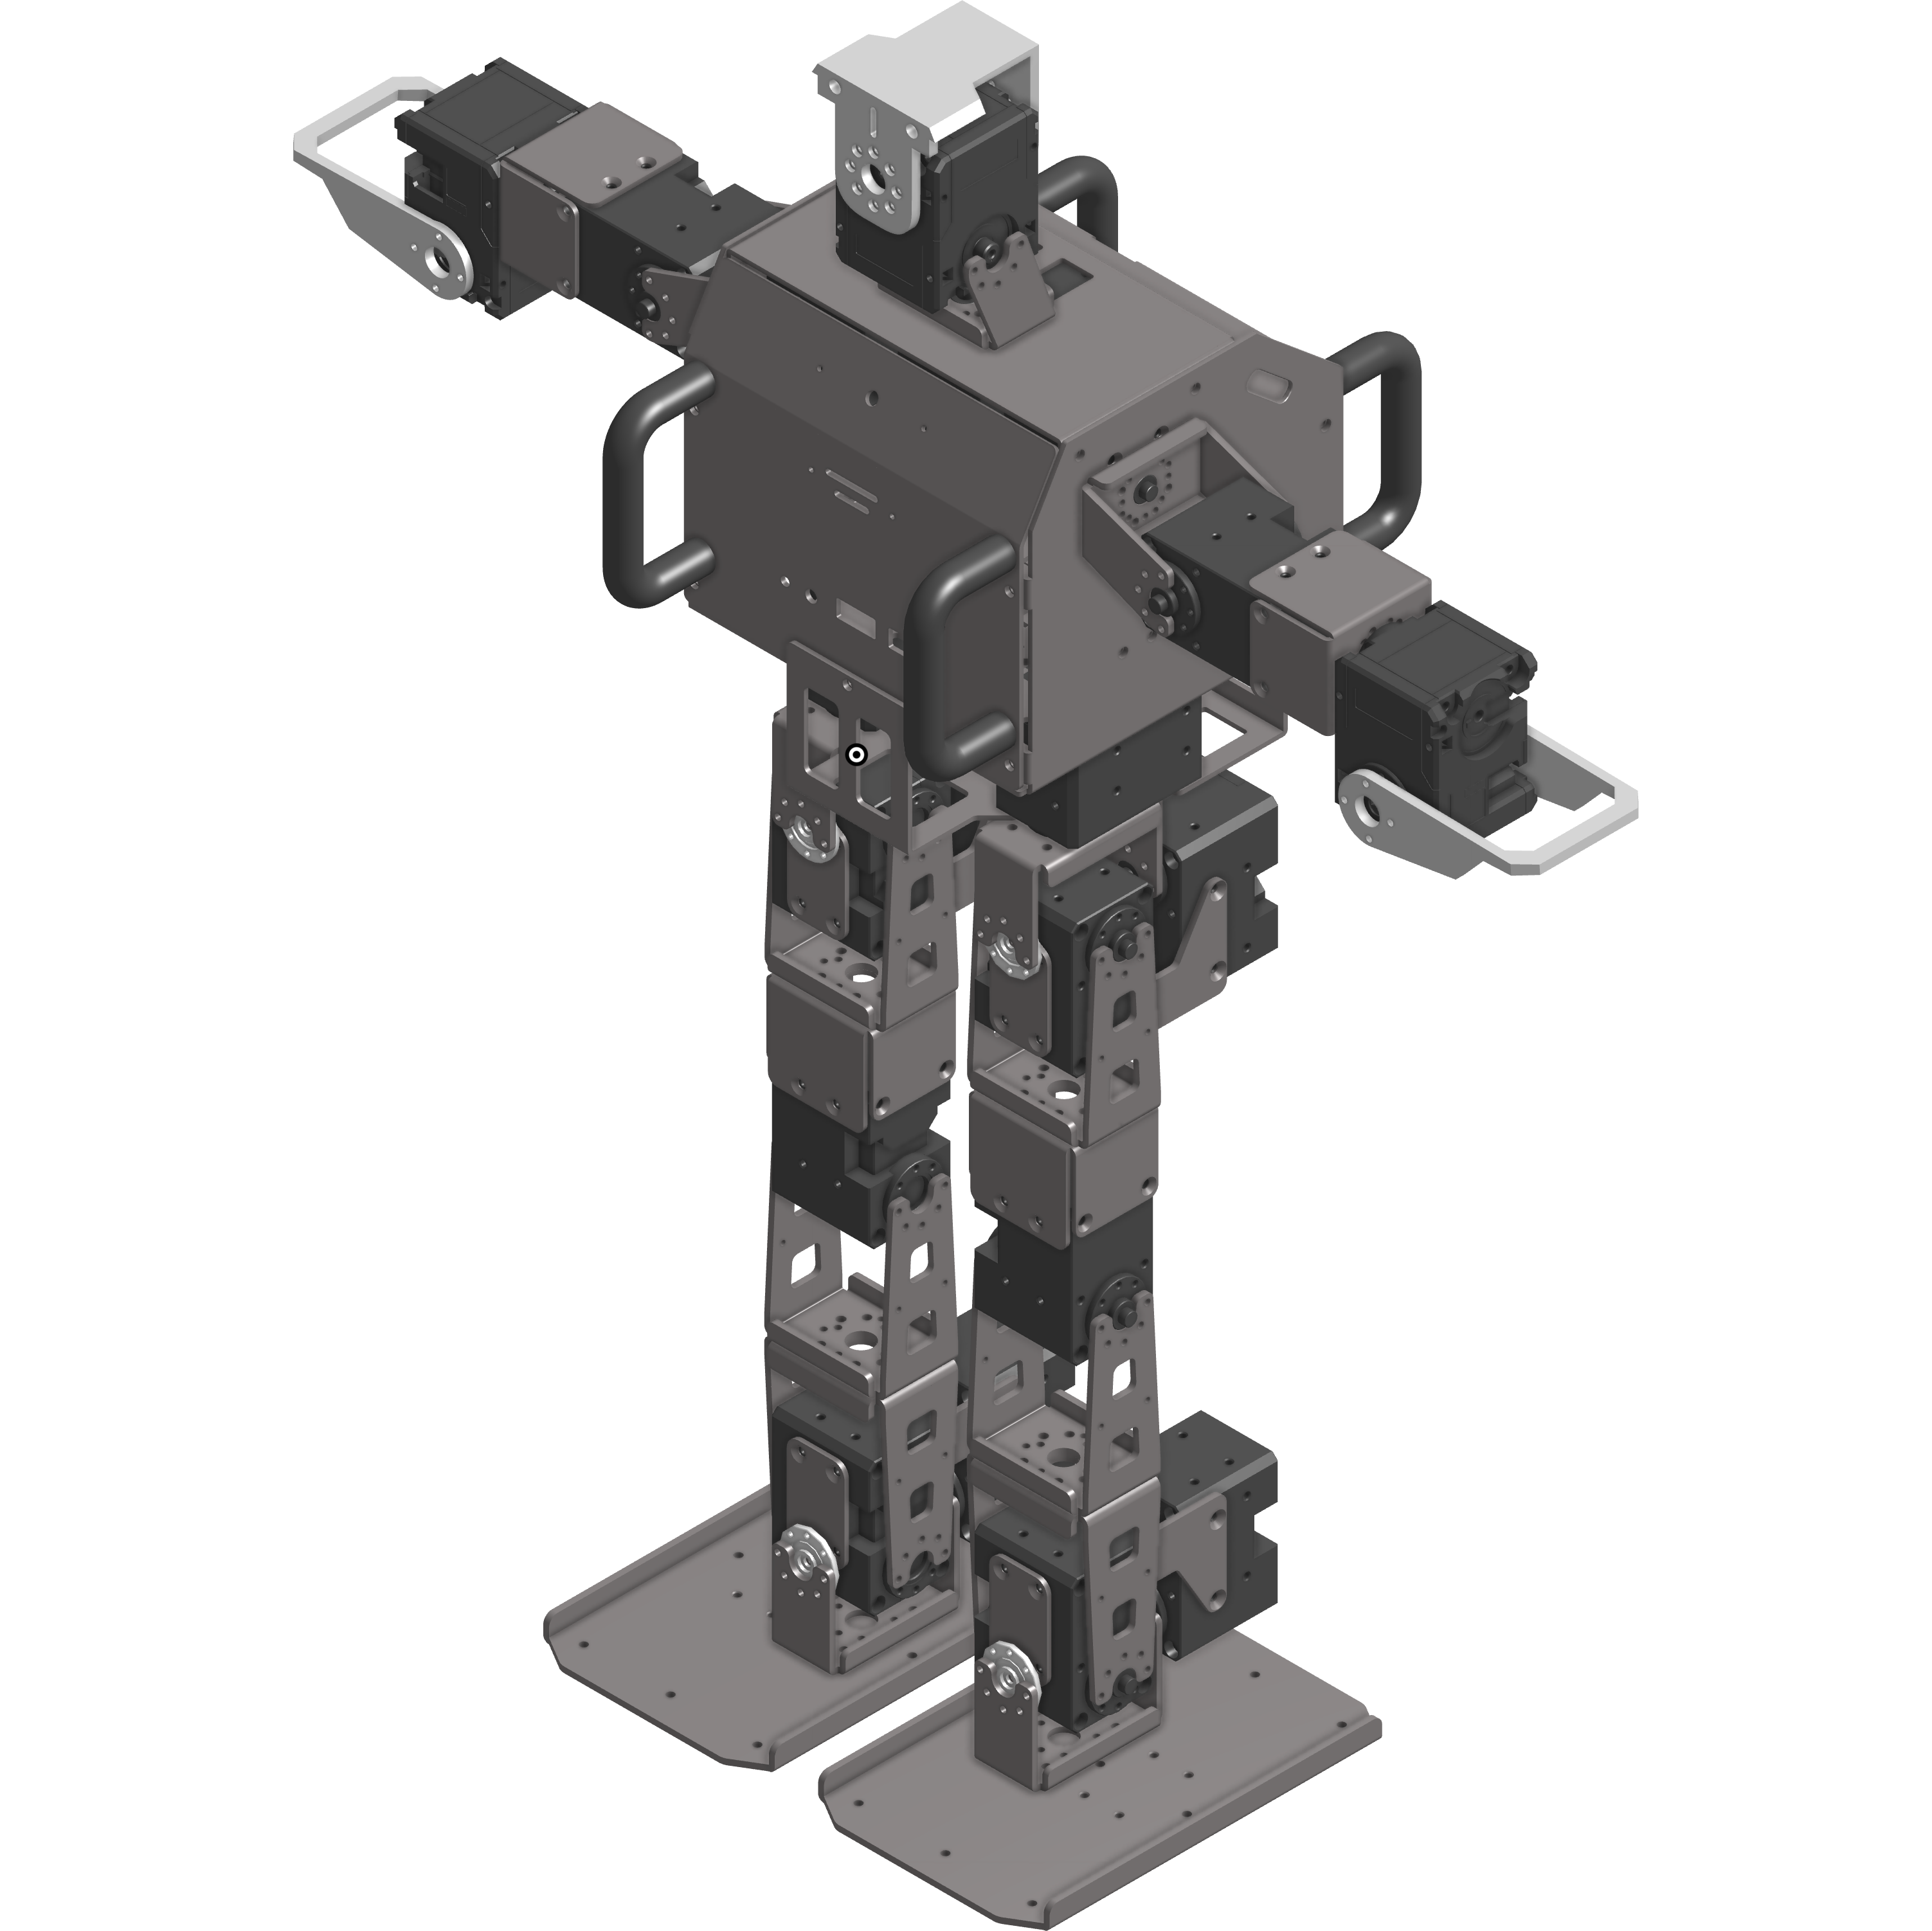
\includegraphics[width=\linewidth]{images/mod_robot1.png}
        \caption*{(a) Tampilan Robotis OP3 - Sisi Isometrik}
    \end{minipage}
    \hfill
    \begin{minipage}{0.48\textwidth}
        \centering
        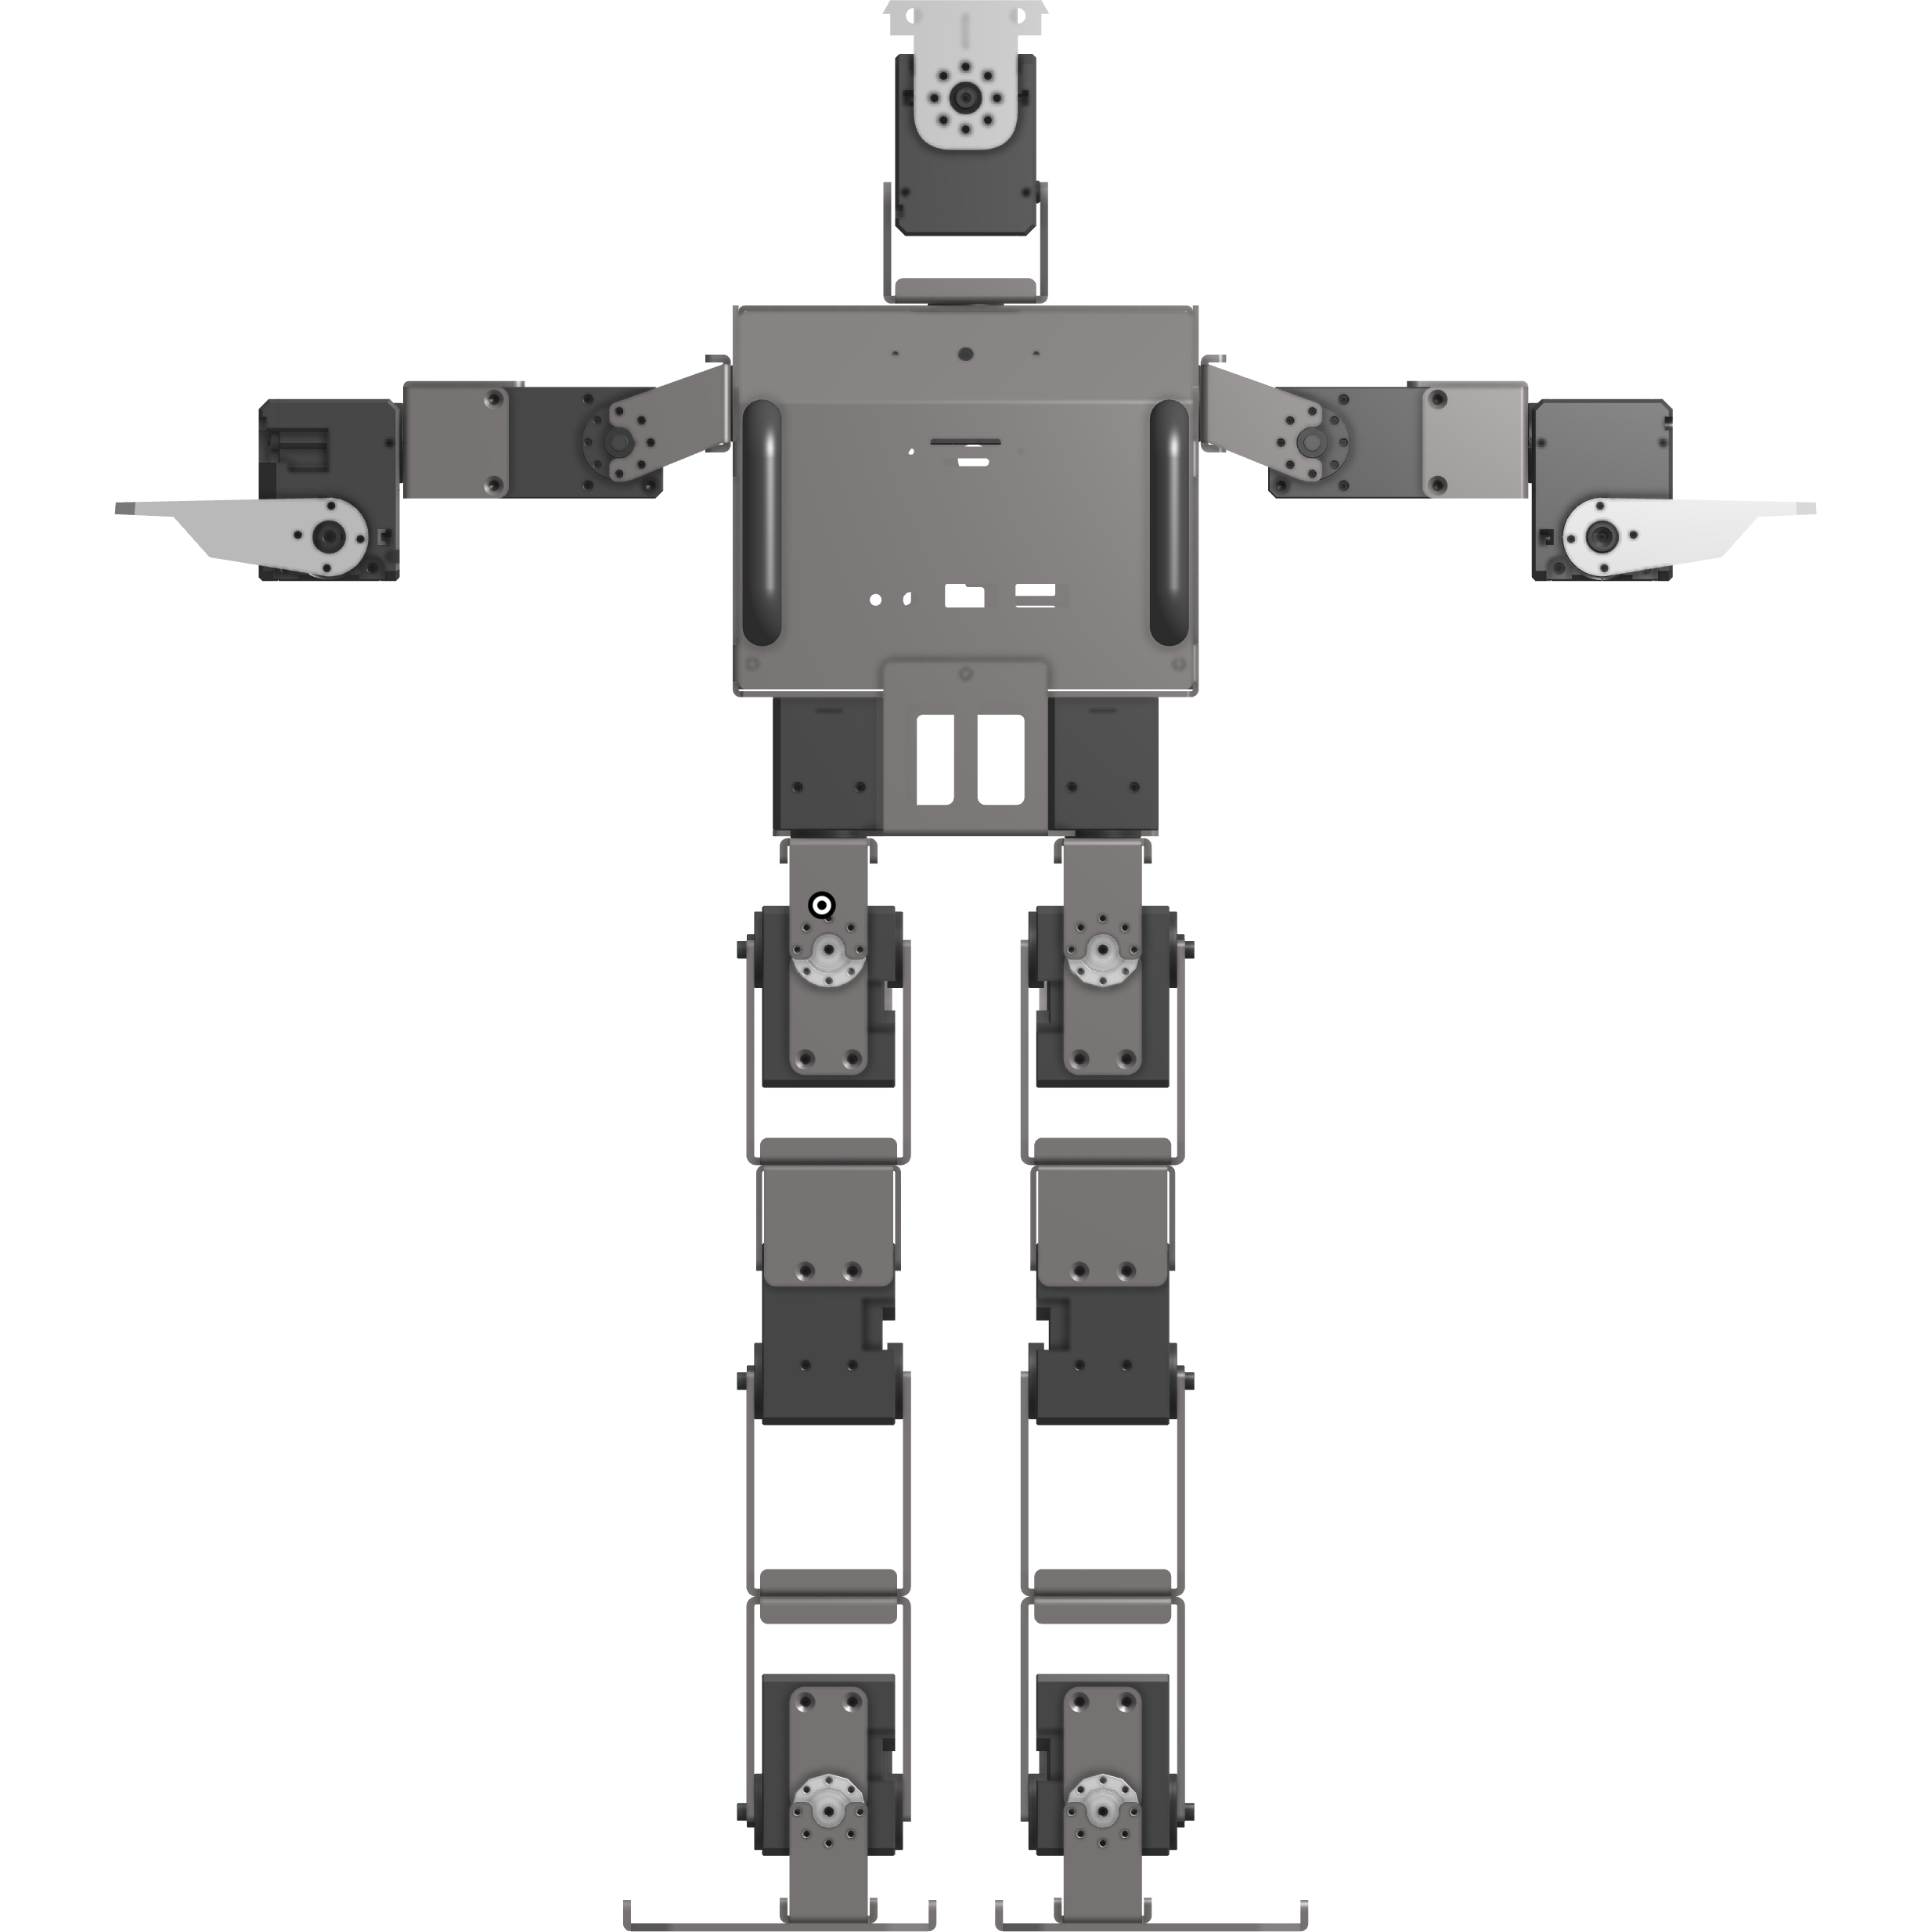
\includegraphics[width=\linewidth]{images/mod_robot2.png}
        \caption*{(b) Tampilan Robotis OP3 - Sisi Depan}
    \end{minipage}
    \caption{Tampilan fisik robot ROBOTIS-OP3 setelah modifikasi}
    \label{fig:modifikasi_fisik}
\end{figure}


Setelah pemasangan, dilakukan kalibrasi awal untuk memastikan sudut nol pada sumbu fleksi dan rotasi sesuai dengan orientasi default robot. Modifikasi fisik ini bertujuan agar robot mampu melakukan gerakan lengan yang lebih kompleks dan proporsional, sehingga mendukung representasi gerakan tari tradisional secara lebih realistis.

\subsection{Implementasi pada Robot}
\subsubsection{Transformasi Koordinat}

\begin{figure}[H]
    \centering
    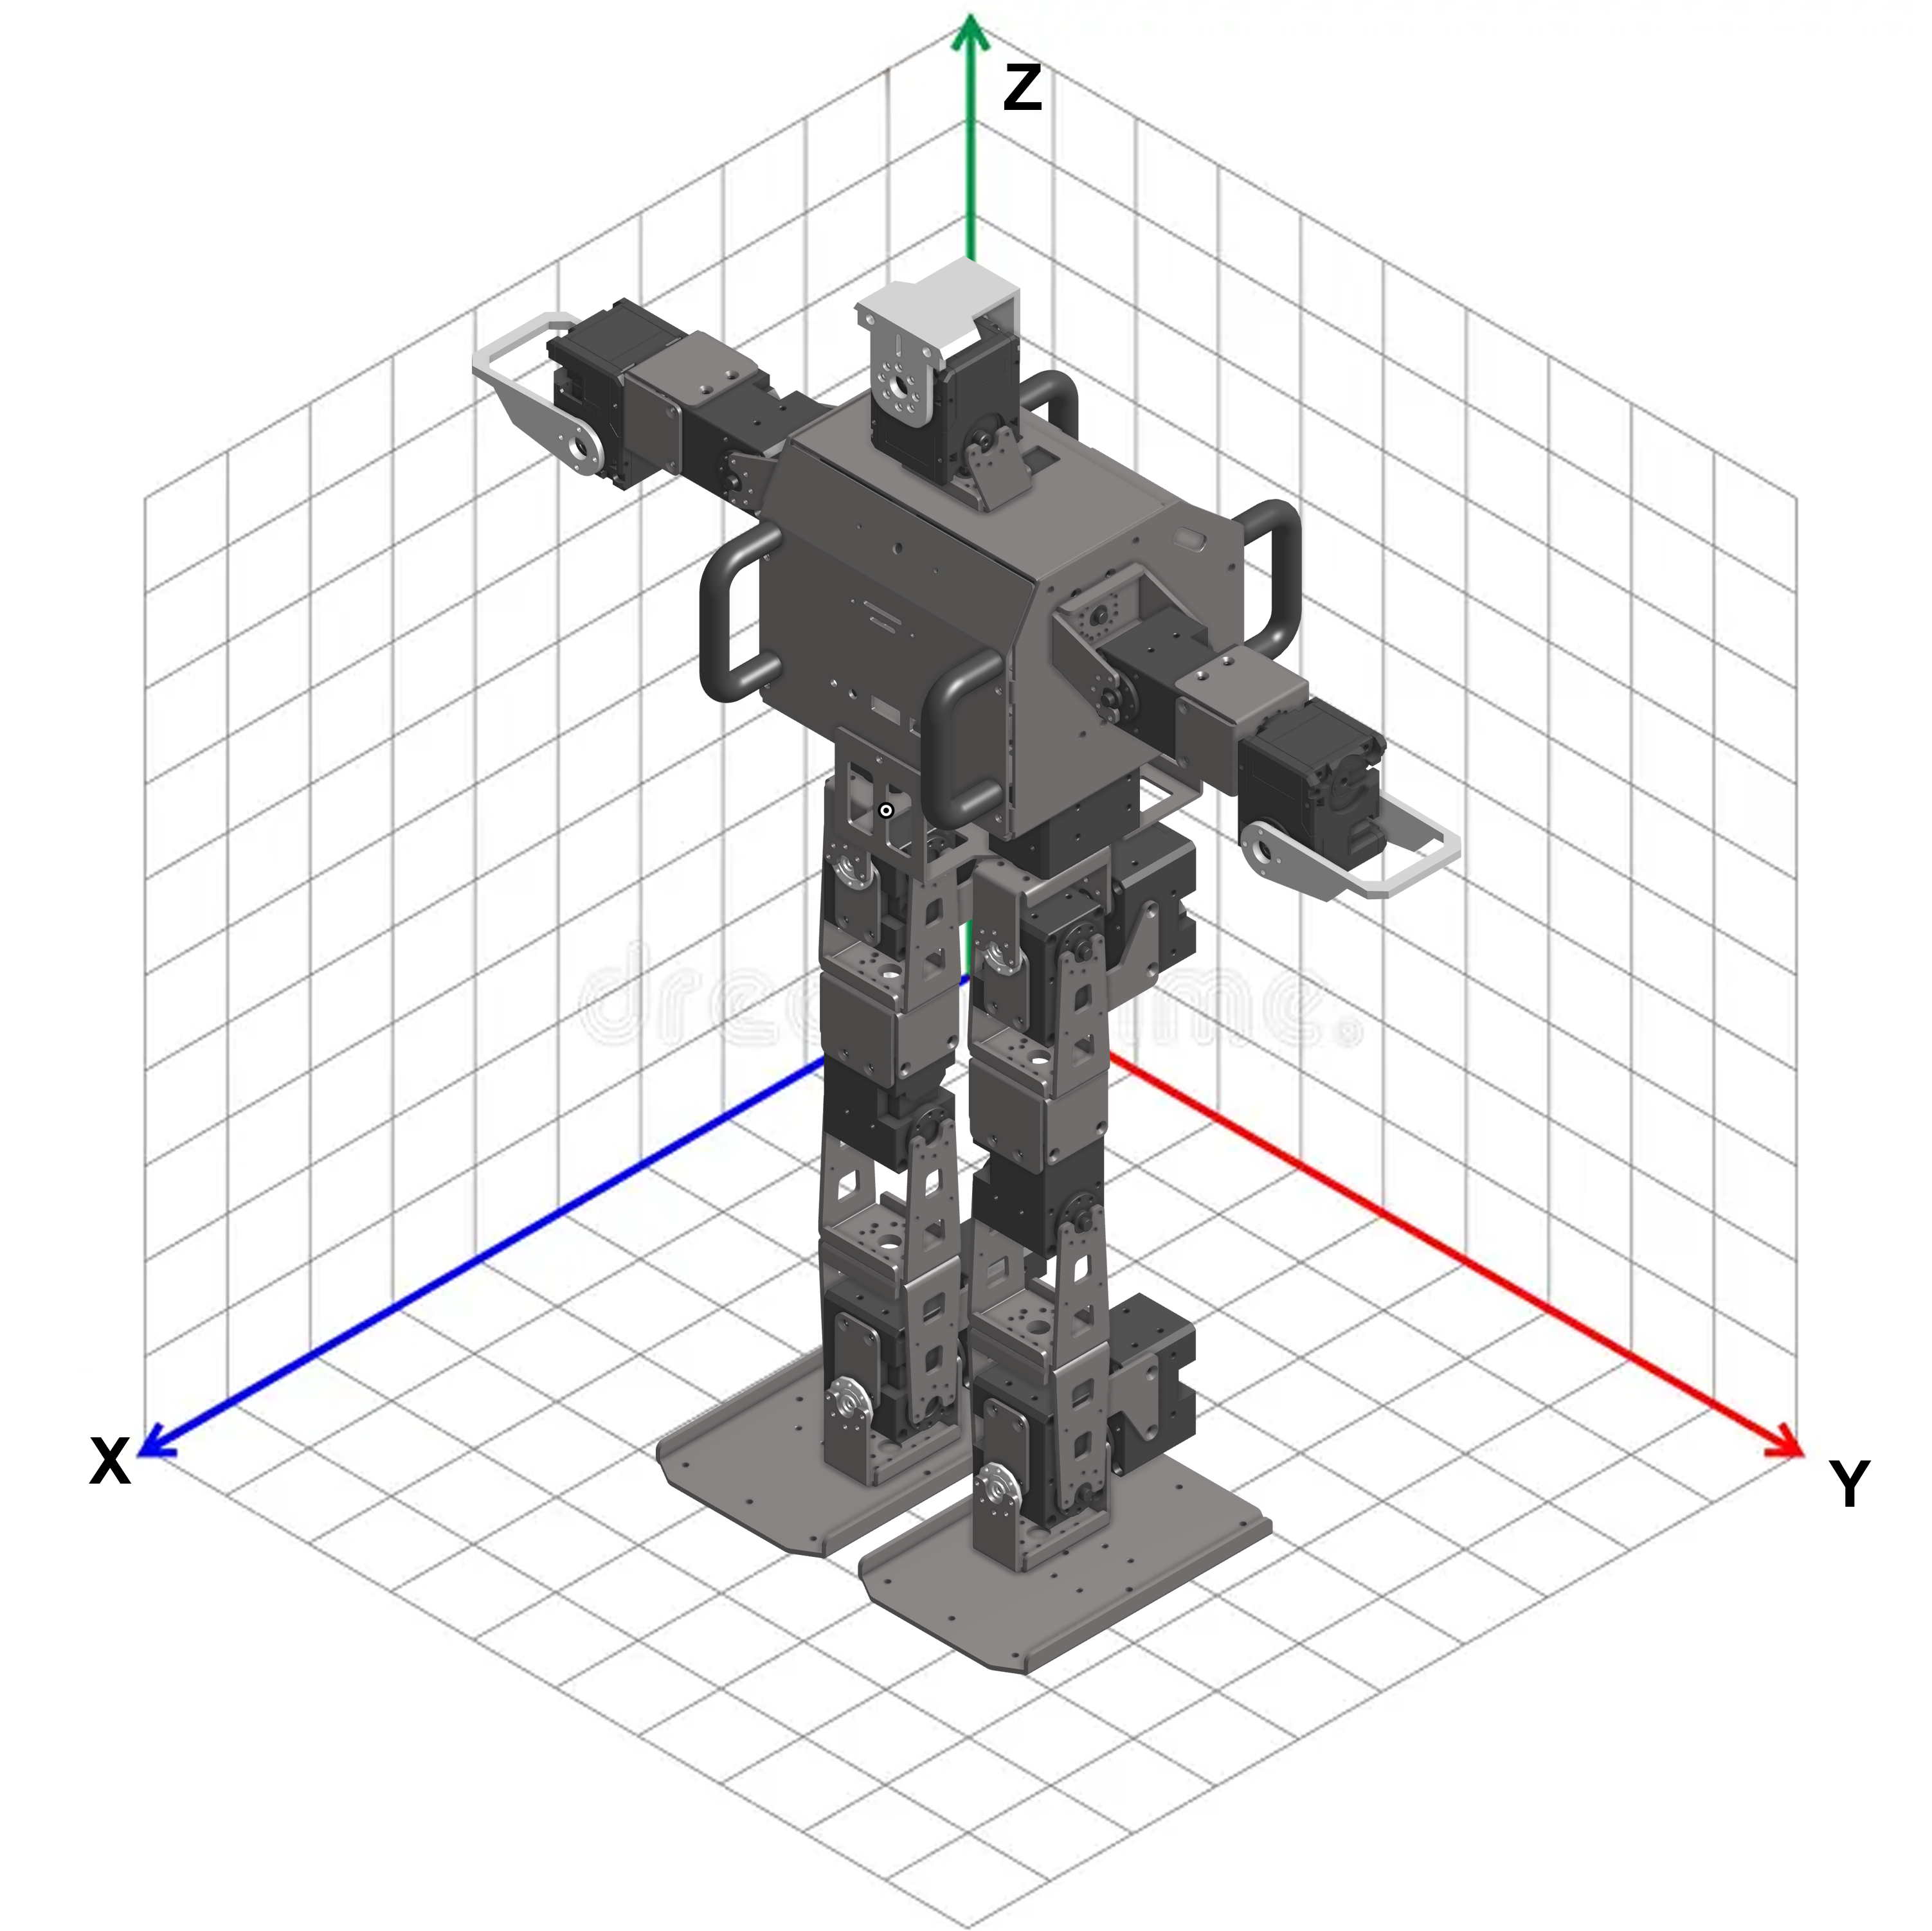
\includegraphics[width=0.6\textwidth]{images/mod_robot_coordinate.png}
    \caption{Visualisasi sistem koordinat robot}
    \label{fig:sistem_koordinat_robot}
\end{figure}

Karena terdapat perbedaan struktur mekanik, panjang sambungan, jumlah derajat kebebasan, serta sistem koordinat antara lengan manusia dan lengan robot ROBOTIS-OP3, maka koordinat 3D hasil estimasi pose tidak dapat langsung diterapkan secara langsung ke sistem kontrol robot. Untuk itu, diperlukan proses transformasi koordinat agar data pose manusia dapat diadaptasikan ke dalam sistem koordinat robot.

Transformasi yang dilakukan pada penelitian ini tidak melibatkan perubahan skala atau translasi global, melainkan hanya penyesuaian orientasi sumbu agar sesuai dengan definisi sumbu pada robot ROBOTIS-OP3. Pada sistem koordinat hasil estimasi pose, orientasi sumbu mengikuti konvensi kamera dengan:

\begin{itemize}
    \item Sumbu X sebagai kiri-kanan,
    \item Sumbu Y sebagai atas-bawah,
    \item Sumbu Z sebagai depan-belakang.
\end{itemize}

Sedangkan pada sistem koordinat robot ROBOTIS-OP3, orientasi sumbu diubah menjadi:

\begin{itemize}
    \item Sumbu X menjadi maju-mundur,
    \item Sumbu Y menjadi kiri-kanan,
    \item Sumbu Z menjadi atas-bawah.
\end{itemize}

Proses transformasi dilakukan dengan menukar posisi sumbu sesuai kebutuhan agar sistem koordinat manusia dapat dipetakan dengan benar ke sistem koordinat robot.

Selain penyesuaian orientasi sumbu, transformasi juga dilakukan untuk memindahkan posisi skeleton pose ke titik referensi yang diketahui, yaitu pada pusat koordinat (0,0,0). Hal ini bertujuan untuk menghilangkan translasi global atau pergeseran posisi dari pose manusia, sehingga seluruh gerakan hanya dihitung relatif terhadap titik tengah yang berupa bahu. Dengan menjadikan skeleton berada di titik nol, sistem hanya memproses perubahan orientasi dan sudut pergerakan, tanpa mempengaruhi posisi absolut di ruang global. Hal ini sesuai dengan implementasi pada robot, di mana pergerakan dilakukan secara \textit{in-place} dengan robot tidak berpindah tempat, hanya menggerakkan lengan dan kepala.


Hubungan transformasi koordinat untuk memetakan titik-titik tubuh manusia ke sistem koordinat robot dirumuskan sebagai berikut:

\begin{equation}
J'_{i} = \mathbf{A} \cdot (J_{i} - J_{1}), \quad i = 1,2,3
\end{equation}

\begin{equation}
J'_{i} = \mathbf{A} \cdot (J_{i} - J_{4}), \quad i = 4,5,6
\end{equation}

\begin{equation}
J'_{i} = \mathbf{A} \cdot (J_{i} - J_{7}), \quad i = 7,8
\end{equation}

Dengan penjelasan sebagai berikut:

\begin{itemize}
    \item $J_i$ merupakan koordinat titik kunci tubuh manusia dalam sistem koordinat dunia, sedangkan $J'_i$ adalah koordinat hasil transformasi dalam sistem koordinat robot.
    \item Matriks $\mathbf{A}$ adalah matriks rotasi yang dibentuk berdasarkan bidang segitiga yang menghubungkan bahu kiri ($J_1$), bahu kanan ($J_4$), dan panggul sebagai referensi.
\end{itemize}

Adapun penomoran titik kunci tubuh adalah sebagai berikut:

\begin{itemize}
    \item $J_{1}, J_{2}, J_{3}$ : Titik pada {lengan kiri}, secara berurutan meliputi \textit{shoulder left}, \textit{elbow left}, dan \textit{wrist left}.
    \item $J_{4}, J_{5}, J_{6}$ : Titik pada {lengan kanan}, secara berurutan meliputi \textit{shoulder right}, \textit{elbow right}, dan \textit{wrist right}.
    \item $J_{7}, J_{8}$ : Titik pada {kepala}, secara berurutan meliputi \textit{neck}, \textit{head}.
\end{itemize}

Transformasi ini dilakukan untuk memastikan bahwa seluruh pergerakan tubuh manusia dapat dipetakan secara tepat ke dalam sistem koordinat robot, dengan mempertimbangkan perbedaan orientasi sumbu dan struktur anatomi antara manusia dan robot. Proses ini memungkinkan perhitungan sudut sendi dilakukan secara konsisten dan sesuai dengan konfigurasi kinematika robot.

Proses transformasi koordinat tidak hanya melibatkan pergeseran titik referensi, tetapi juga pembentukan matriks rotasi $A$ yang berfungsi untuk menyelaraskan orientasi tubuh manusia dengan sistem koordinat robot. Matriks ini dibentuk berdasarkan tiga vektor ortonormal yang merepresentasikan arah sumbu lokal tubuh manusia, yaitu arah kiri-kanan, depan-belakang, dan atas-bawah.

Pembuatan matriks $A$ dilakukan dengan langkah-langkah sebagai berikut:

\begin{enumerate}
    \item Hitung vektor sumbu $z$ sebagai arah tegak lurus tubuh dari panggul($J_{9}$) ke pertengahan bahu:
    
    \begin{equation}
    {z} = \frac{(J_1 + J_4)}{2} - J_9
    \end{equation}
    
    Normalisasi vektor $z$ menjadi vektor unit:
    
    \begin{equation}
    {z}_{\text{axis}} = \frac{{z}}{||{z}||}
    \end{equation}
    
    \item Hitung vektor sumbu $y$ sebagai vektor dari bahu kanan ke bahu kiri:
    
    \begin{equation}
    {y} = J_1 - J_4
    \end{equation}
    
    Normalisasi vektor $y$ menjadi vektor unit:
    
    \begin{equation}
    {y}_{\text{axis}} = \frac{{y}}{||{y}||}
    \end{equation}
    
    \item Hitung vektor sumbu $x$ sebagai hasil perkalian silang antara ${y}_{\text{axis}}$ dan ${z}_{\text{axis}}$:
    
    \begin{equation}
    {x}_{\text{axis}} = {y}_{\text{axis}} \times {z}_{\text{axis}}
    \end{equation}
    
    Normalisasi vektor $x$ menjadi vektor unit:
    
    \begin{equation}
    {x}_{\text{axis}} = \frac{{x}_{\text{axis}}}{||{x}_{\text{axis}}||}
    \end{equation}
    
    \item Lakukan re-orthogonalization pada ${y}_{\text{axis}}$ agar tetap tegak lurus terhadap ${z}_{\text{axis}}$ dan ${x}_{\text{axis}}$:
    
    \begin{equation}
    {y}_{\text{axis}} = {z}_{\text{axis}} \times {x}_{\text{axis}}
    \end{equation}
    
    Normalisasi kembali:
    
    \begin{equation}
    {y}_{\text{axis}} = \frac{{y}_{\text{axis}}}{||{y}_{\text{axis}}||}
    \end{equation}
    
    \item Susun ketiga vektor ortonormal menjadi matriks rotasi $A$ sebagai berikut:
    
    \begin{equation}
    \mathbf{A} =
    \begin{bmatrix}
    x_1 & y_1 & z_1 \\
    x_2 & y_2 & z_2 \\
    x_3 & y_3 & z_3 \\
    \end{bmatrix}
    \end{equation}
    
    di mana ${x}_{\text{axis}} = [x_1, x_2, x_3]^T$, ${y}_{\text{axis}} = [y_1, y_2, y_3]^T$, dan ${z}_{\text{axis}} = [z_1, z_2, z_3]^T$.
\end{enumerate}


Matriks $\mathbf{A}$ ini digunakan untuk mentransformasikan koordinat dari sistem global (kamera) ke sistem lokal tubuh yang telah disesuaikan dengan orientasi robot. Proses ini memastikan bahwa orientasi sumbu tubuh manusia selaras dengan sistem koordinat robot, sehingga perhitungan sudut sendi dapat dilakukan secara konsisten dan akurat.


\subsubsection{Konversi Pose 3D ke Sudut Sendi}

Setelah koordinat pose 3D diselaraskan ke dalam sistem koordinat robot, langkah selanjutnya adalah menghitung sudut-sudut sendi berdasarkan arah vektor lengan atas, lengan bawah dan kepala. Sudut yang dihitung mencakup dua sudut pada bahu (\textit{pitch} dan \textit{roll}), dua sudut pada siku (\textit{twist} dan \textit{flexion}), dan 3 sudut pada kepala (\textit{pan}, \textit{tilt}, \textit{roll}). Proses ini memanfaatkan fungsi trigonometri invers dan operasi aljabar vektor.

Vektor lengan atas dan lengan bawah dapat didefinisikan sebagai:

\begin{equation}
\vec{V}_{\text{up}} = J'_{\text{elbow}} - J'_{\text{shoulder}} = 
\begin{bmatrix}
v^{up}_x \\
v^{up}_y \\
v^{up}_z
\end{bmatrix}
\end{equation}

\begin{equation}
\vec{V}_{\text{low}} = J'_{\text{wrist}} - J'_{\text{elbow}} = 
\begin{bmatrix}
v^{low}_x \\
v^{low}_y \\
v^{low}_z
\end{bmatrix}
\end{equation}

Sudut \textit{Shoulder Pitch} pada lengan kiri dinotasikan sebagai $\theta_{\text{LSPitch}}$, dihitung menggunakan fungsi $\arctan2$ terhadap komponen $-x$ dan $-z$ dari vektor lengan atas. Penggunaan tanda negatif pada kedua komponen dilakukan untuk menyelaraskan arah rotasi dengan orientasi sumbu pada robot, sehingga pergerakan yang dihasilkan sesuai dengan konfigurasi servo pada lengan kiri. Rumus perhitungan $\theta_{\text{LSPitch}}$ adalah sebagai berikut:

\begin{equation}
\theta_{\text{LSPitch}} = \arctan2\left(-v^{up}_x, -v^{up}_z\right)
\end{equation}

Sudut \textit{Shoulder Roll} pada lengan kiri dinotasikan sebagai $\theta_{\text{LSRoll}}$. Perhitungan sudut ini digunakan untuk mengetahui seberapa jauh lengan kiri bergerak ke samping (ke atas atau ke bawah). Sudut dihitung menggunakan fungsi $\arctan2$ sebagai berikut:

\begin{equation}
\theta_{\text{LSRoll}} = \arctan2\left(\sqrt{(v^{up}_x)^2 + (v^{up}_z)^2}, v^{up}_y\right)
\end{equation}

Perhitungan sudut $\theta_{\text{LEYaw}}$ dan $\theta_{\text{LERoll}}$ memerlukan transformasi koordinat lanjutan, yaitu dari sistem koordinat bahu kiri ke sistem koordinat siku kiri. Transformasi ini diperlukan agar perhitungan sudut di siku dilakukan secara lokal terhadap orientasi lengan atas. Hal tersebut didapatkan dengan melakukan rotasi pada vektor lebgan bawah dengan dua matriks rotasi berurutan, yaitu matriks $R_y$ dan matriks $R_x$ untuk mengoreksi orientasi terhadap sudut $\theta_{\text{LSPitch}}$ dan $\theta_{\text{LSRoll}}$.

\begin{equation}
\vec{V}'_{\text{low}} = R_x \cdot R_y \cdot \vec{v}_{\text{low}}
\end{equation}

Transformasi ini menghasilkan vektor lengan bawah dalam kerangka koordinat baru yang telah disejajarkan dengan orientasi lengan atas, sehingga sudut $-\theta_{\text{LEYaw}}$ dan $-\theta_{\text{LERoll}}$ dapat dihitung dengan lebih akurat.

Matriks rotasi $R_y$ dan $R_x$ masing-masing dituliskan sebagai berikut:

\begin{equation}
R_y(-\theta_{\text{LSPitch}}) = 
\begin{bmatrix}
\cos(-\theta_{\text{LSPitch}}) & 0 & \sin(-\theta_{\text{LSPitch}}) \\
0 & 1 & 0 \\
-\sin(-\theta_{\text{LSPitch}}) & 0 & \cos(-\theta_{\text{LSPitch}})
\end{bmatrix}
\end{equation}

\begin{equation}
R_x(-\theta_{\text{LSRoll}}) = 
\begin{bmatrix}
1 & 0 & 0 \\
0 & \cos(-\theta_{\text{LSRoll}}) & \sin(-\theta_{\text{LSRoll}}) \\
0 & -\sin(-\theta_{\text{LSRoll}}) & \cos(-\theta_{\text{LSRoll}})
\end{bmatrix}
\end{equation}

Tanda negatif pada setiap sudut digunakan untuk menyesuaikan arah rotasi dari sistem koordinat manusia ke sistem koordinat robot, agar sesuai dengan pergerakan fisik servo pada ROBOTIS-OP3.

Sudut \textit{Elbow Twist} pada lengan kiri dinotasikan sebagai $\theta_{\text{LETwist}}$, dihitung dari komponen vektor lengan bawah hasil rotasi. Perhitungan dilakukan menggunakan fungsi $\arctan2$ sebagai berikut:

\begin{equation}
\theta_{\text{LETwist}} = \arctan2\left(v'^{low}_x,v'^{low}_z\right)
\end{equation}

Sedangkan sudut \textit{Elbow Flexion} pada lengan kiri dinotasikan sebagai $\theta_{\text{LEFlex}}$, dihitung berdasarkan sudut antara vektor lengan atas dan vektor lengan bawah dengan menggunakan rumus dot product sebagai berikut:

\begin{equation}
\theta_{\text{LEFlex}} = \arctan2\left(-\sqrt{(v'^{low}_x)^2 + (v'^{low}_z)^2},v'^{low}_y\right)
\end{equation}

Perhitungan ini digunakan untuk menentukan seberapa besar lengan bawah menekuk (\textit{flexion}) dan berputar (\textit{twist}) relatif terhadap lengan atas dalam kerangka lokal yang telah disejajarkan.

Implementasi dari proses ini dilakukan pada kode program dengan memanfaatkan operasi vektor sederhana, seperti perkalian silang, dot product, dan normalisasi, yang diikuti dengan fungsi trigonometri $\arctan2$ dan $\arccos$. Langkah ini memastikan sudut yang diperoleh sesuai dengan batas pergerakan fisik servo pada robot humanoid ROBOTIS-OP3.


\begin{lstlisting}[style=plainbox, caption={Implementasi perhitungan sudut sendi sesuai rumus}]
aup_L = J_elbow - J_shoulder
alow_L = J_wrist - J_elbow

LShoulderPitch = np.arctan2(-aup_L[0], -aup_L[2])  # (X, Z)
LShoulderRoll = np.arctan2(np.sqrt(aup_L[0]**2 + aup_L[2]**2),
                 aup_L[1]
                 )

Ry = np.array([
    [np.cos(-LShoulderPitch), 0, np.sin(-LShoulderPitch)],
    [0, 1, 0],
    [-np.sin(-LShoulderPitch), 0, np.cos(-LShoulderPitch)]
])

Rx = np.array([
    [1, 0, 0],
    [0, np.cos(-LShoulderRoll), np.sin(-LShoulderRoll)],
    [0, -np.sin(-LShoulderRoll),  np.cos(-LShoulderRoll)]
])
alow_L_prime = Rx @ Ry @ alow_L
LElbowPitch = np.arctan2(-alow_L_prime[0], -alow_L_prime[2])
LElbowRoll = np.arctan2(
    -np.sqrt(alow_L_prime[0]**2 + alow_L_prime[2]**2),
    alow_L_prime[1]
)

ElbowFlexion = -np.degrees(angle_between_vectors(auJ_L, alow_L))
\end{lstlisting}
Begitu juga dengan bagian kepala, untuk mendapatkan sudut orientasi kepala, pertama-tama didefinisikan vektor kepala sebagai selisih antara posisi titik kepala dan titik leher:

\begin{equation}
\vec{V}_{\text{head}} = J'_{\text{head}} - J'_{\text{neck}} = 
\begin{bmatrix}
v^{head}_x \\[3pt]
v^{head}_y \\[3pt]
v^{head}_z
\end{bmatrix}
\end{equation}

Sudut \textit{Head Pan} dinotasikan sebagai $\theta_{\text{HPan}}$, yang merepresentasikan rotasi mendatar kepala (gerakan menengok ke kiri dan kanan). Sudut ini dihitung menggunakan fungsi $\arctan2$ terhadap komponen $y$ dan $x$ dari vektor kepala:

\begin{equation}
\theta_{\text{HPan}} = \arctan2\left(v^{head}_y, v^{head}_x\right)
\end{equation}

Sudut \textit{Head Roll} dinotasikan sebagai $\theta_{\text{HRoll}}$, yang menunjukkan kemiringan kepala ke samping (memiringkan kepala kiri atau kanan). Perhitungan dilakukan dengan:

\begin{equation}
\theta_{\text{HRoll}} = -\arctan2\left(v^{head}_y, v^{head}_z\right)
\end{equation}

Sedangkan sudut \textit{Head Tilt} atau \textit{Head Pitch}, dinotasikan sebagai $\theta_{\text{HTilt}}$, digunakan untuk mendeskripsikan gerakan kepala mendongak atau menunduk. Perhitungan dilakukan sebagai berikut:

\begin{equation}
\theta_{\text{HTilt}} = \arctan2\left(v^{head}_x, v^{head}_z\right)
\end{equation}

Perhitungan ketiga sudut ini dilakukan dalam kerangka lokal tubuh yang telah disesuaikan dengan orientasi robot, sehingga pergerakan kepala yang dihasilkan dapat sesuai dengan arah rotasi servo pada bagian kepala ROBOTIS-OP3.

\begin{lstlisting}[style=plainbox, caption={Implementasi perhitungan sudut kepala}]
ahead = J_head - J_neck  # vektor kepala
HeadPan = (np.arctan2(ahead[1], ahead[0]))
HeadRoll = -(np.arctan2(ahead[1], ahead[2]))
HeadTilt = (np.arctan2(ahead[0], ahead[2]))
\end{lstlisting}
\subsection{Penyimpanan Gerakan dalam Format JSON}

Setelah seluruh sudut sendi berhasil dihitung untuk setiap frame pose 3D, data gerakan kemudian disimpan dalam format berkas {JSON}. Penyimpanan ini bertujuan untuk memudahkan proses pemutaran ulang gerakan pada robot, serta sebagai format pertukaran data yang sederhana dan mudah diakses. Pada tahap ini, setiap frame hasil konversi disusun dalam struktur data Python \textit{dictionary}, dengan penamaan kunci yang sesuai dengan nama sendi pada robot. Contoh pemetaan sudut sendi ke nama kunci JSON dapat dilihat berikut:

\begin{lstlisting}[style=plainbox, caption={Pemetaan hasil sudut ke format JSON}]
frame_result = {
    "r_sho_pitch": angles_R["ShoulderPitch"],
    "l_sho_pitch": angles_L["ShoulderPitch"],
    "r_sho_roll": angles_R["ShoulderRoll"],
    "l_sho_roll": angles_L["ShoulderRoll"],
    "r_el_pitch": angles_R["ElbowTwist"],
    "l_el_pitch": angles_L["ElbowTwist"],
    "r_el_roll": angles_R["ElbowFlexion"],
    "l_el_roll": angles_L["ElbowFlexion"],
    "head_pan": angles_head["HeadPan"],
    "head_pitch": angles_head["HeadTilt"],
    "head_roll": angles_head["HeadRoll"],
}

results[str(frame_idx)] = frame_result
\end{lstlisting}

Setelah seluruh frame diproses, data hasil konversi disimpan dalam berkas {JSON} menggunakan fungsi {json.dump()}. Berikut contoh kode penyimpanan:

\begin{lstlisting}[style=plainbox, caption={Penyimpanan hasil gerakan dalam file JSON}]
output_file = "/home/luthfai/Devel/skripsi/pose_angles2.json"
with open(output_file, "w") as f:
    json.dump(results, f, indent=2)
\end{lstlisting}

Format file {JSON} ini berisi daftar sudut sendi per frame dalam satuan derajat, yang kemudian dapat digunakan sebagai masukan untuk perintah gerakan pada robot humanoid ROBOTIS-OP3.
Contoh isi file JSON hasil penyimpanan dapat dilihat pada Potongan Data berikut:

\begin{lstlisting}[style=plainbox, caption={Contoh data sudut sendi dalam format JSON}]
{
  "0": {
    "r_sho_pitch": -7.799538951688305,
    "l_sho_pitch": -10.71019173677621,
    "r_sho_roll": -46.40881222111872,
    "l_sho_roll": 48.35393974799908,
    "r_el_pitch": 121.56508280420996,
    "l_el_pitch": -103.9285816547141,
    "r_el_roll": -32.71889721964388,
    "l_el_roll": -17.327496671902992,
    "head_pan": -15.129533767700195,
    "head_pitch": -2.2988436222076416,
    "head_roll": 1.3416086435317993
  },
}
\end{lstlisting}

Data ini menunjukkan sudut sendi dalam satuan derajat untuk frame ke-0 pose 3D, yang kemudian dapat diproses sebagai perintah gerakan robot.

\subsection{Eksekusi Gerakan pada Robot}

Tahap akhir dalam sistem ini adalah menjalankan pergerakan lengan robot berdasarkan data sudut sendi yang telah dikonversi dan disimpan dalam berkas JSON. Proses ini dilakukan dengan memuat data sudut untuk setiap frame, mengonversi sudut derajat menjadi nilai posisi servo Dynamixel, kemudian mengirimkan perintah posisi ke semua aktuator secara sinkron.

File JSON yang berisi urutan sudut sendi dibaca dan diurutkan berdasarkan nomor frame. Data sudut kemudian dikonversi menggunakan fungsi \textit{deg\_to\_dxl} untuk menghasilkan nilai posisi servo yang sesuai dengan protokol pengendalian Dynamixel. Hasil konversi disimpan dalam variabel \textit{joint\_trajectories} yang memuat data untuk seluruh frame.

Pada tahap playback, program melakukan iterasi melalui setiap frame. Nilai posisi servo dikirimkan ke aktuator menggunakan metode write4ByteTxRx() atau melalui mekanisme sinkronisasi paket (\textit{sync write}), sehingga semua sendi bergerak serempak sesuai dengan urutan gerakan yang diinginkan. Kecepatan eksekusi dapat diatur menggunakan fungsi sleep() untuk mengatur interval antar frame.

Contoh kode Python yang digunakan dalam proses eksekusi gerakan robot adalah sebagai berikut:

\begin{lstlisting}[style=plainbox, caption={Kode eksekusi playback gerakan pada robot humanoid}]
for frame_idx in range(len(angle_data)):
    for joint_name, joint_id in JOINTS.items():
        pos = joint_trajectories[joint_name][frame_idx]

        # Konversi posisi menjadi 4 byte
        param_goal_position = [
            DXL_LOBYTE(DXL_LOWORD(pos)),
            DXL_HIBYTE(DXL_LOWORD(pos)),
            DXL_LOBYTE(DXL_HIWORD(pos)),
            DXL_HIBYTE(DXL_HIWORD(pos))
        ]
        groupSyncWrite.addParam(joint_id, 
                                bytearray(param_goal_position)
                                )
    groupSyncWrite.txPacket()
    groupSyncWrite.clearParam()

    time.sleep(1.0 / 30.0)
\end{lstlisting}

Proses ini memastikan robot dapat mereplikasi urutan gerakan hasil estimasi pose secara konsisten dengan kecepatan yang telah ditentukan.



\section{Implementasi Website}

Website yang dikembangkan pada penelitian ini berfungsi sebagai antarmuka utama untuk memproses video gerakan tari, melakukan estimasi pose 3D, menyimpan hasil konversi sudut, serta mengirim perintah gerakan ke robot humanoid. Sistem website dikembangkan menggunakan framework Flask, sedangkan proses inferensi model pose estimation dijalankan secara terpisah menggunakan Uvicorn dan FastAPI. Pemisahan ini dilakukan karena lingkungan Python untuk model estimasi membutuhkan pustaka tambahan seperti TensorFlow dan Torch yang berbeda versi dengan dependensi Flask.

Saat aplikasi pertama kali dijalankan, pengguna akan diarahkan pada halaman utama yang menampilkan judul Video Pose Estimation di bagian atas. Di sisi kiri halaman terdapat area unggah video, dengan ikon upload berukuran besar sebagai pusat interaksi. Bagian ini memungkinkan pengguna memilih video gerakan tari tradisional yang akan diproses. Setelah file dipilih, nama video akan muncul pada area log di bagian kanan bawah halaman, sehingga pengguna dapat memastikan bahwa file berhasil dimuat. Tampilan awal antarmuka website dapat dilihat pada Gambar~\ref{fig:website_awal}.

\begin{figure}[H]
    \centering
    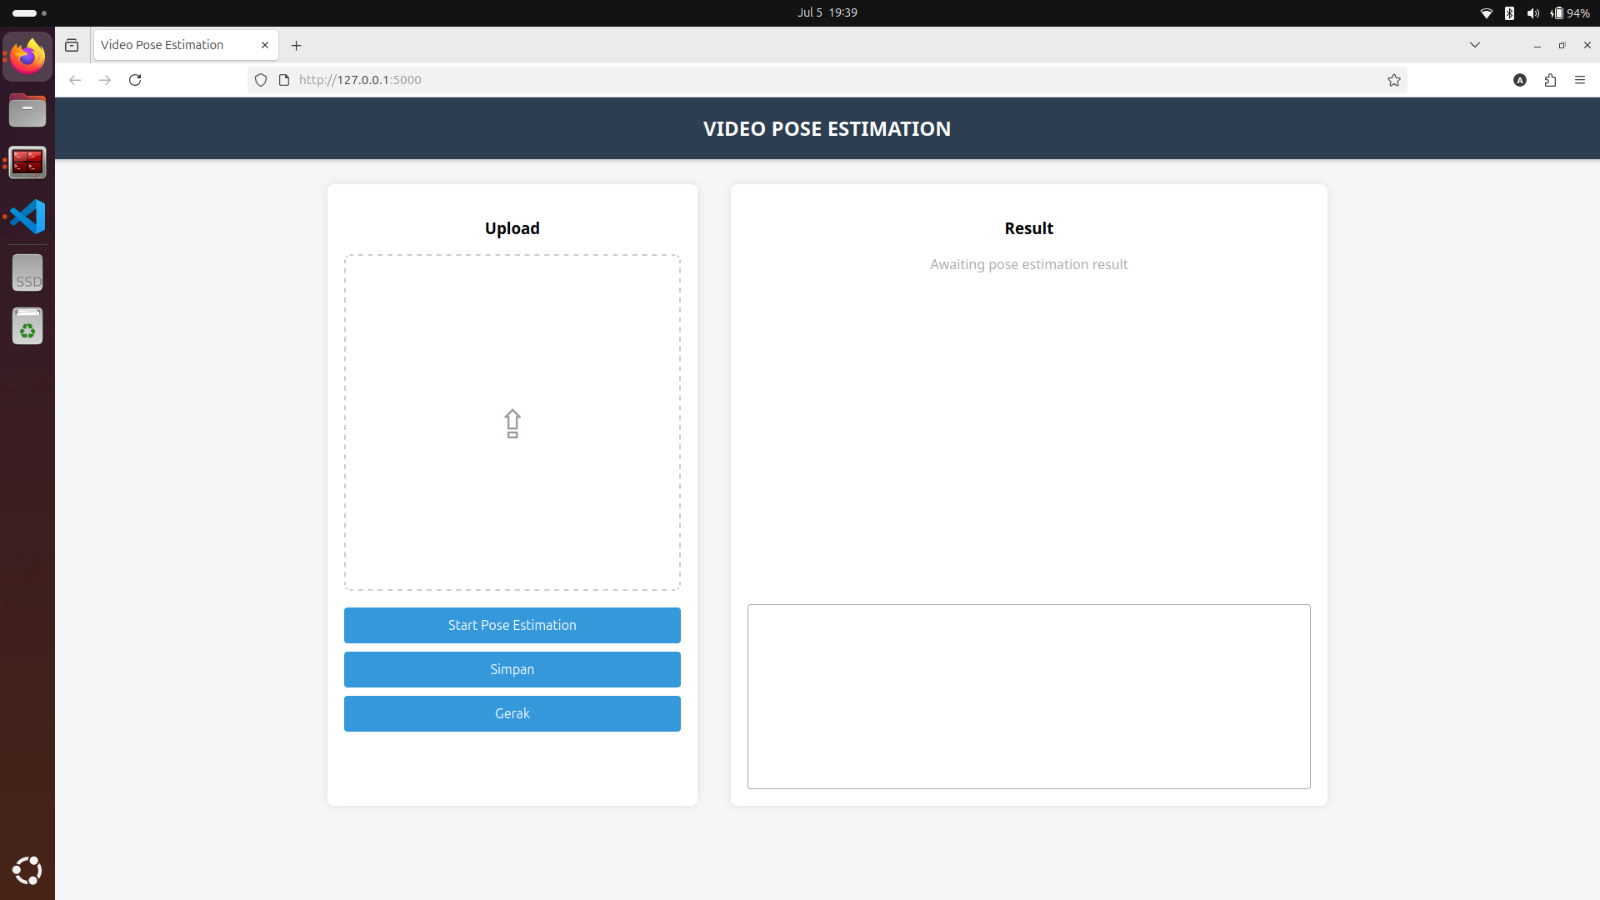
\includegraphics[width=0.9\textwidth]{images/tampilan1.jpeg}
    \caption{Tampilan awal website sebelum interaksi pengguna}
    \label{fig:website_awal}
\end{figure}

Pengguna dapat mengunggah video gerakan tari tradisional melalui tombol unggah. Setelah video dipilih, sistem akan menampilkan nama file pada area log. Contoh tampilan proses pemilihan video ditunjukkan pada Gambar~\ref{fig:upload_video}.

\begin{figure}[H]
    \centering
    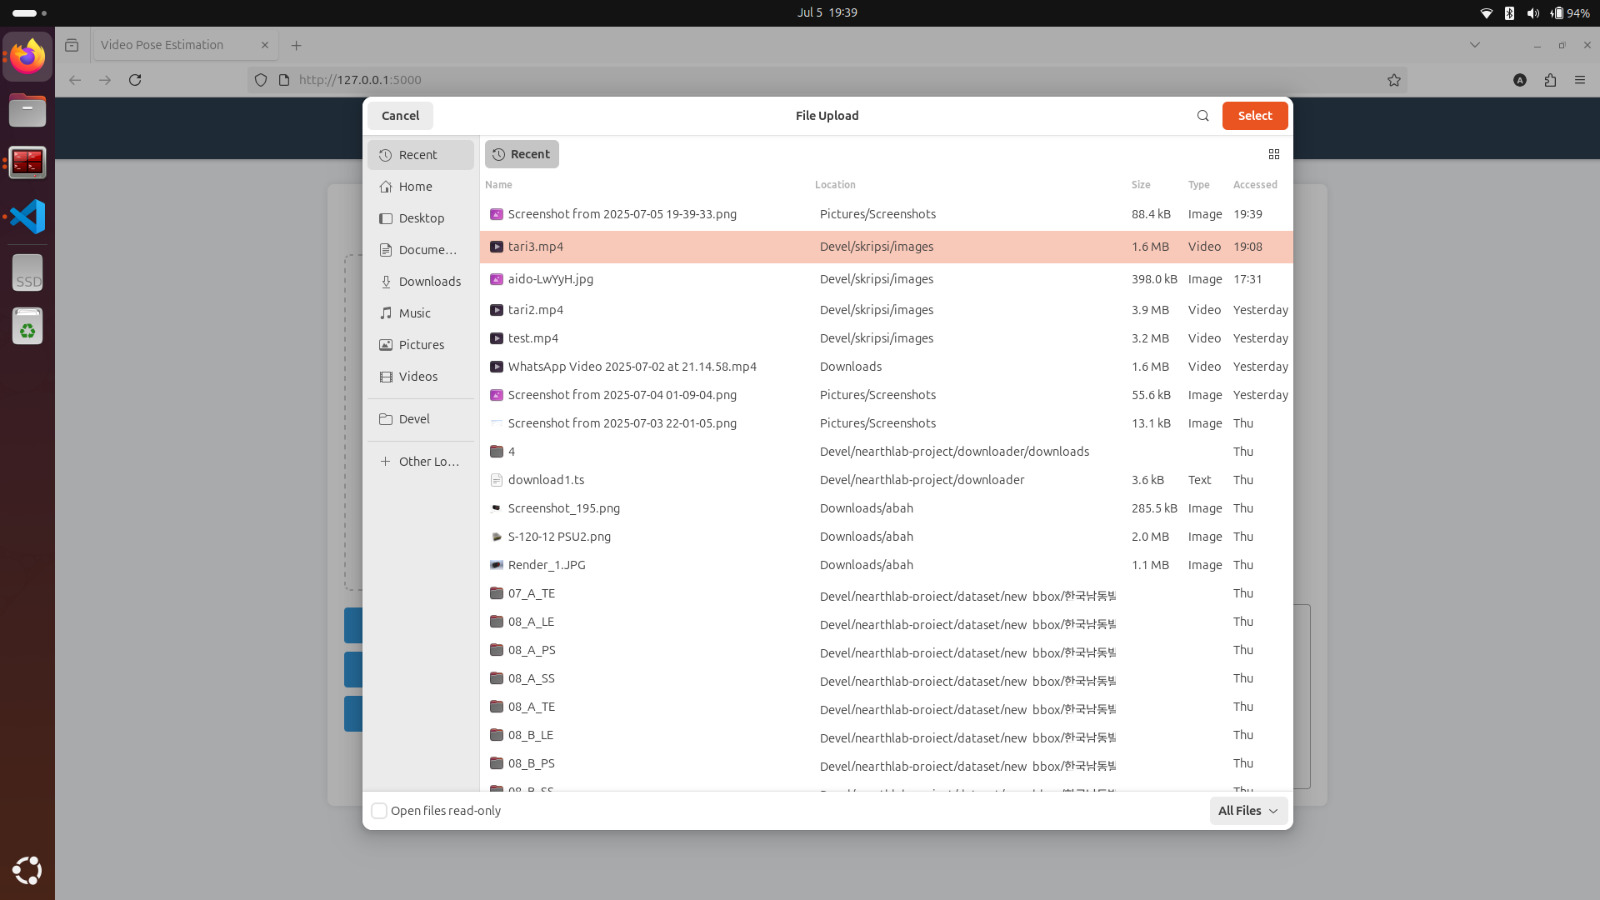
\includegraphics[width=0.9\textwidth]{images/tampilan2.jpeg}
    \caption{Proses upload dan pemilihan video}
    \label{fig:upload_video}
\end{figure}

Setelah video berhasil diunggah, pengguna dapat menekan tombol Start Pose Estimation yang terletak di bawah area unggah video. Ketika tombol ini ditekan, sistem akan melakukan proses estimasi pose 3D pada video secara bertahap. Proses ini dijalankan oleh server Uvicorn yang secara independen menangani komputasi model TensorFlow. Selama proses inferensi berlangsung, sistem menampilkan progress log dan visualisasi kerangka pose yang diperbarui secara real-time. Gambar~\ref{fig:proses_estimasi_pose} menunjukkan contoh tampilan proses estimasi pose.

\begin{figure}[H]
    \centering
    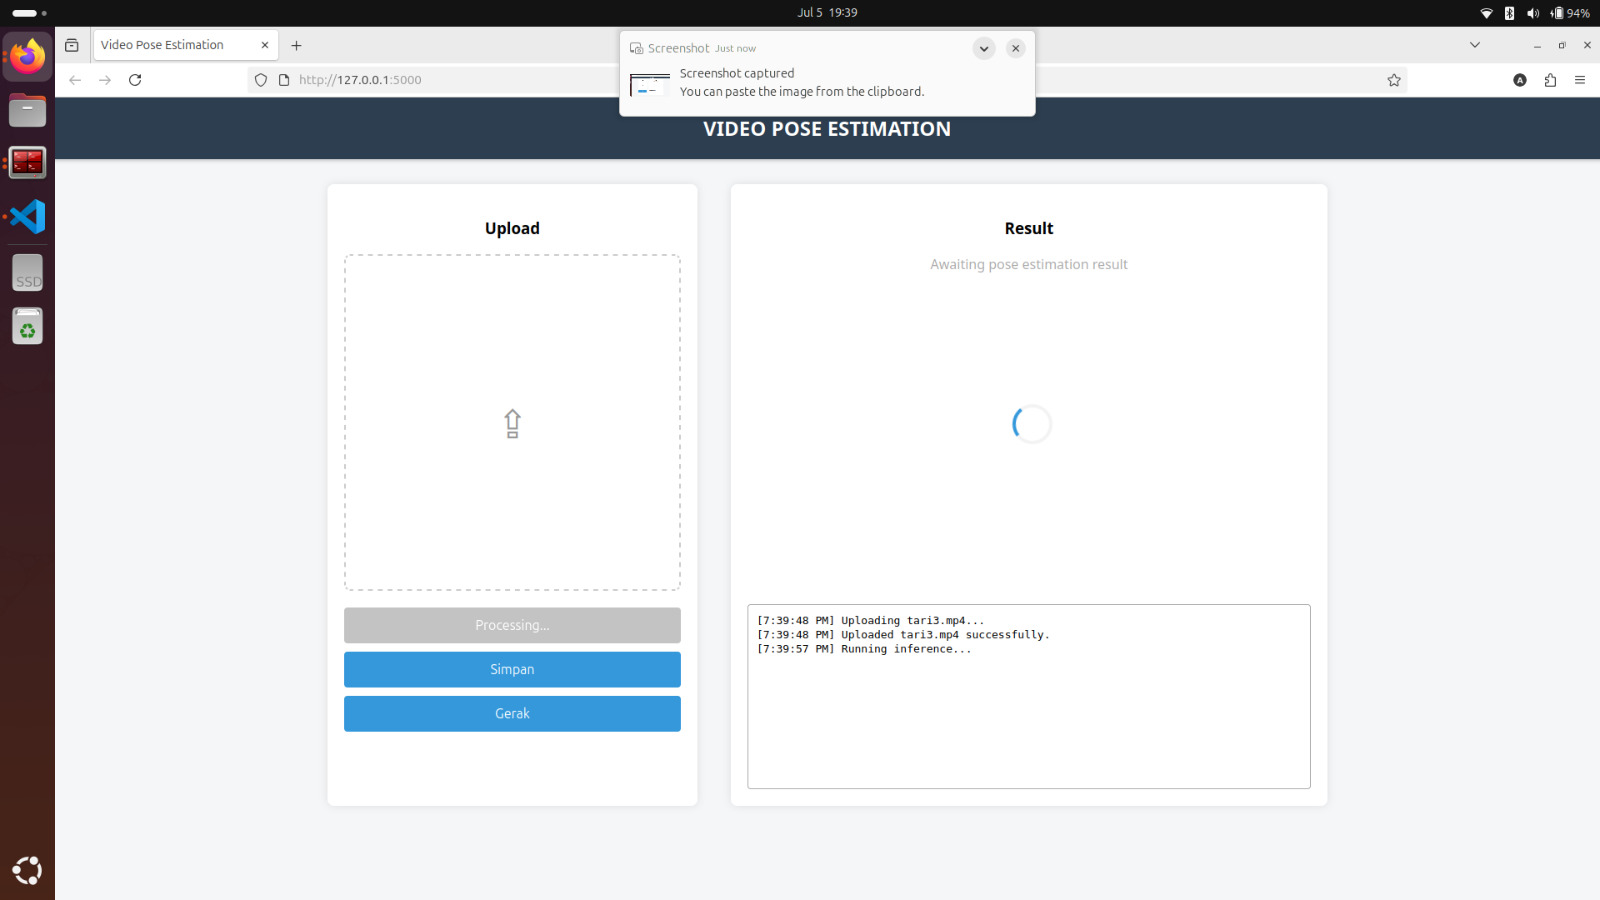
\includegraphics[width=0.9\textwidth]{images/tampilan4.jpeg}
    \caption{Tampilan proses estimasi pose 3D sedang berjalan}
    \label{fig:proses_estimasi_pose}
\end{figure}

Setelah estimasi selesai, hasil prediksi pose akan divisualisasikan dalam bentuk skeleton 3D pada sisi kanan halaman. Visualisasi ini dilengkapi keterangan frame saat ini dan total jumlah frame, sehingga pengguna dapat memantau hasil pose estimation secara lebih detail. Contoh hasil visualisasi ditunjukkan pada Gambar~\ref{fig:hasil_estimasi_pose}.

\begin{figure}[H]
    \centering
    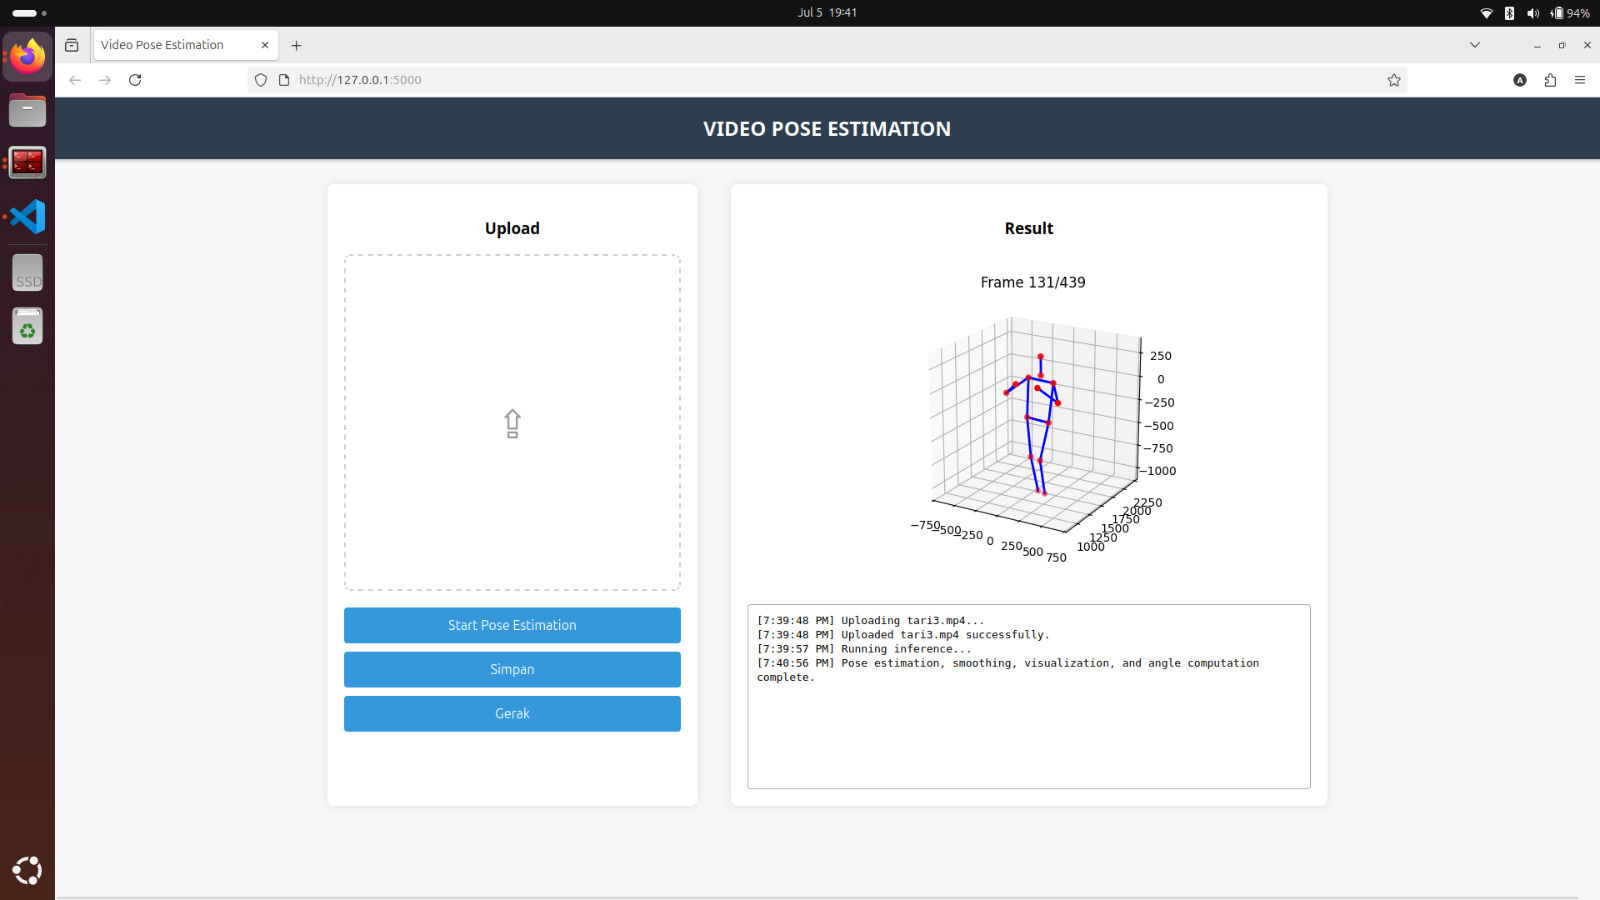
\includegraphics[width=0.9\textwidth]{images/tampilan5.jpeg}
    \caption{Hasil visualisasi pose 3D setelah proses estimasi selesai}
    \label{fig:hasil_estimasi_pose}
\end{figure}

Di bagian bawah area unggah video, terdapat tombol Simpan dan Gerak. Tombol Simpan digunakan untuk menyimpan hasil konversi sudut sendi dalam format JSON. File JSON yang dihasilkan berisi nilai sudut sendi untuk setiap frame, yang kemudian dapat digunakan sebagai input gerakan robot. Setelah penyimpanan selesai, sistem akan menampilkan notifikasi log yang menginformasikan direktori penyimpanan file. Contoh tampilan proses penyimpanan ditunjukkan pada Gambar~\ref{fig:simpan_pose}.

\begin{figure}[H]
    \centering
    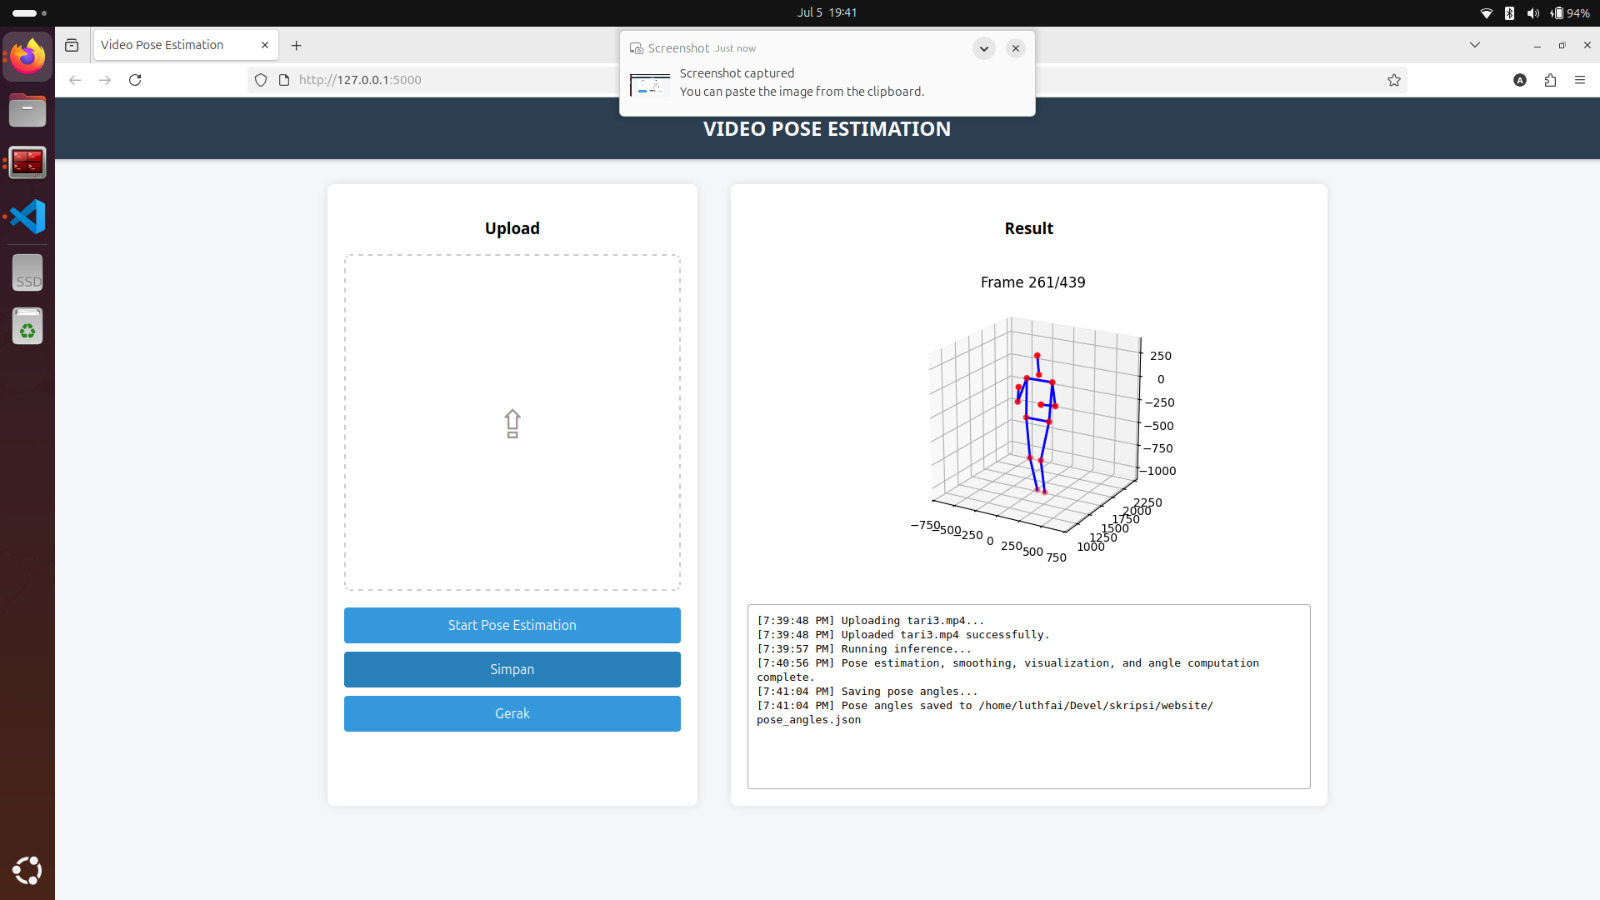
\includegraphics[width=0.9\textwidth]{images/tampilan6.jpeg}
    \caption{Tampilan saat proses penyimpanan data sudut sendi}
    \label{fig:simpan_pose}
\end{figure}

Tombol Gerak digunakan untuk memulai eksekusi playback gerakan pada robot humanoid ROBOTIS-OP3. Saat tombol ini ditekan, sistem akan membaca file JSON yang telah disimpan sebelumnya dan mengirimkan perintah posisi servo secara sinkron melalui protokol Dynamixel. Gambar~\ref{fig:gerakan_robot} menunjukkan tampilan antarmuka ketika proses gerakan robot dijalankan.

\begin{figure}[H]
    \centering
    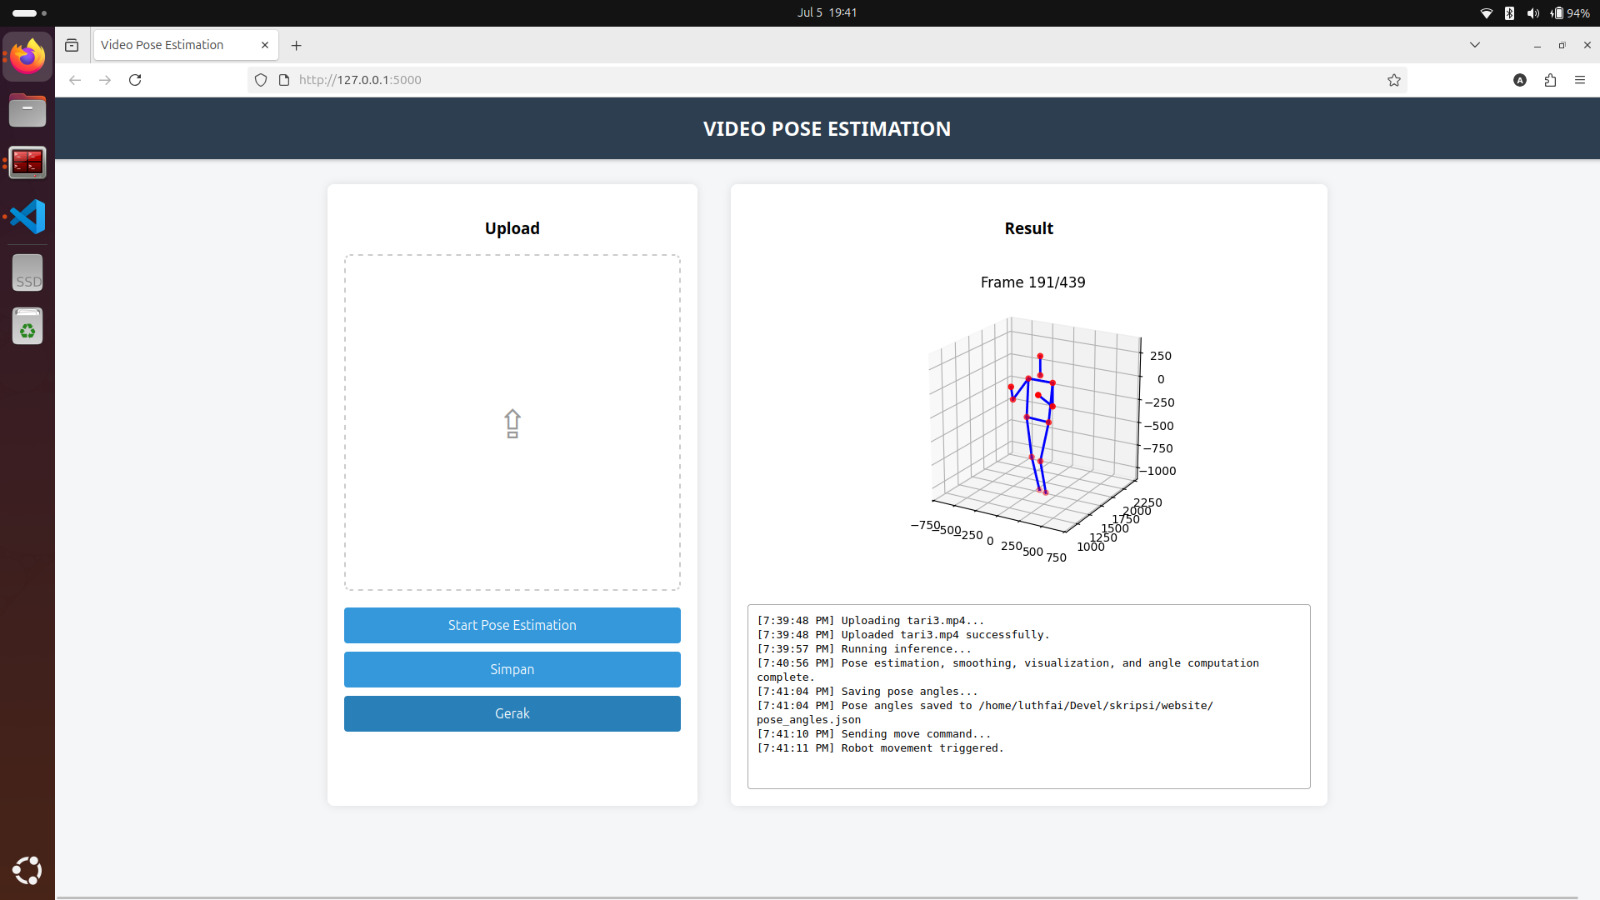
\includegraphics[width=0.9\textwidth]{images/tampilan7.jpeg}
    \caption{Tampilan saat proses playback gerakan robot berjalan}
    \label{fig:gerakan_robot}
\end{figure}

Dengan desain ini, seluruh proses mulai dari unggah video, estimasi pose, penyimpanan sudut sendi, hingga playback gerakan dapat dilakukan secara terpadu melalui satu antarmuka web yang sederhana namun lengkap. Pemisahan server Flask dan Uvicorn memungkinkan sistem berjalan lebih stabil karena proses komputasi model TensorFlow tidak memengaruhi kinerja web server utama.

\section{Pengujian Fungsional Sistem}

Pengujian fungsional dirancang untuk memastikan seluruh fitur utama pada sistem dapat berjalan sesuai dengan spesifikasi yang telah ditentukan. Metode pengujian menggunakan pendekatan \textit{black-box testing}, dengan skenario uji yang disusun berdasarkan masing-masing fitur yang terdapat pada sistem.

Pada tahap ini, pengujian fungsional aplikasi tidak dilakukan secara langsung oleh penulis, melainkan direncanakan untuk dieksekusi oleh anggota tim robotik yang bertugas mengelola implementasi pada perangkat robot. Pengujian ini mencakup alur penggunaan aplikasi, mulai dari input video hingga eksekusi gerakan pada robot ROBOTIS-OP3.

Tabel~\ref{tab:rencana_pengujian_fungsional} berikut menyajikan {rencana skenario pengujian fungsional} yang telah disusun.

\begin{longtable}{|c|p{2.5cm}|p{5cm}|p{4cm}|}
\caption{Rencana Pengujian Fungsional Sistem}
\label{tab:rencana_pengujian_fungsional} \\ \hline
\textbf{No} & \textbf{Fitur} & \textbf{Skenario Pengujian} & \textbf{Hasil yang Diharapkan} \\ \hline
\endfirsthead
\hline
\textbf{No} & \textbf{Fitur} & \textbf{Skenario Pengujian} & \textbf{Hasil yang Diharapkan} \\ \hline
\endhead

1 & Upload Video & Pengguna memilih dan mengunggah file video gerakan tari tradisional. & File berhasil diunggah dan nama file muncul di area log. \\ \hline
2 & Estimasi Pose dan Filtering & Pengguna menekan tombol \textit{Start Pose Estimation}. & Proses estimasi dan filtering berjalan hingga selesai tanpa error. \\ \hline
3 & Tampilan Estimasi Pose & Sistem menampilkan skeleton 3D hasil estimasi setiap frame. & Visualisasi skeleton muncul sesuai urutan frame video. \\ \hline
4 & Status Log & Sistem mencatat status proses pada area log. & Log status muncul pada setiap tahap proses. \\ \hline
5 & Penyimpanan Data & Pengguna menekan tombol \textit{Simpan} setelah estimasi pose selesai. & File JSON disimpan dalam direktori output. \\ \hline
6 & Playback Robot & Pengguna menekan tombol \textit{Gerak} untuk menjalankan robot. & Robot bergerak sesuai data sudut hasil estimasi pose. \\ \hline

\end{longtable}

    \chapter{HASIL DAN PEMBAHASAN}
\vspace{1em}

\section{Hasil dan Pembahasan Sistem}
\subsection{Hasil dan Pembahasan Implementasi pada Robot}
Pada tahap ini dilakukan implementasi sistem ke dalam robot humanoid ROBOTIS-OP3 untuk mereplikasi gerakan manusia berdasarkan hasil estimasi pose yang telah diolah sebelumnya. Proses ini melibatkan beberapa tahapan penting, mulai dari konversi data pose 3D menjadi sudut servo, validasi area pergerakan robot, hingga eksekusi gerakan secara fisik. Berikut adalah pembahasan hasil implementasi pada masing-masing tahap.
\subsubsection{Konversi Koordinat ke Sudut Servo}

\begin{figure}[H]
    \centering
    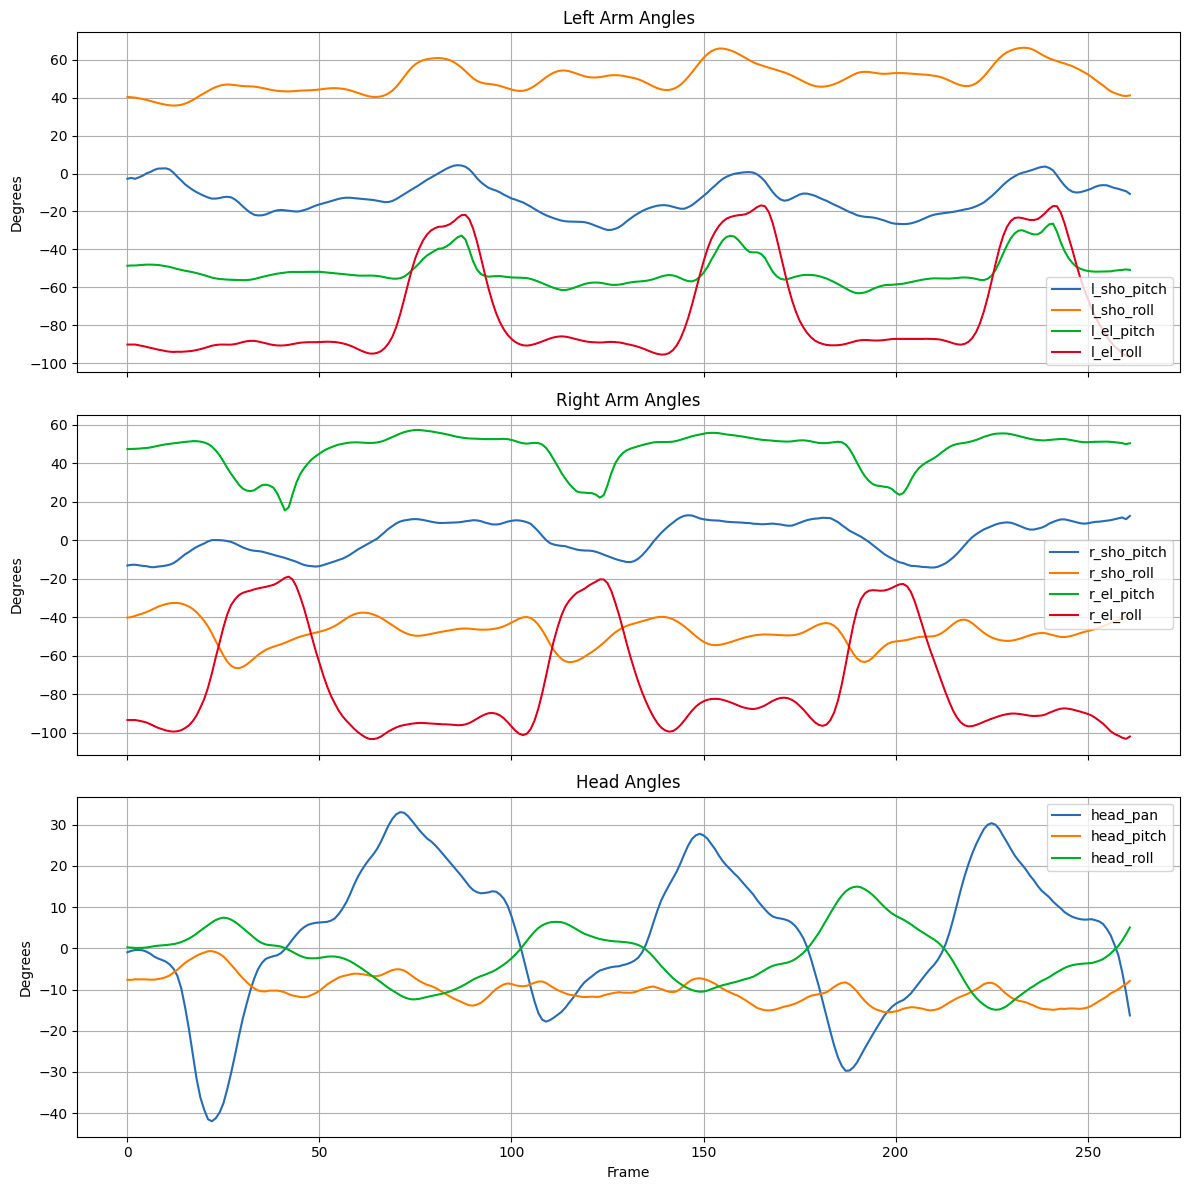
\includegraphics[width=0.7\textwidth]{images/angles_per_joint.png}
    \caption{Grafik perubahan sudut sendi robot per frame pada lengan kiri, lengan kanan, dan kepala}
    \label{fig:angles_per_joint}
\end{figure}

Gambar~\ref{fig:angles_per_joint} menunjukkan hasil visualisasi perubahan sudut sendi (servo) pada robot humanoid untuk mengontrol pergerakan lengan kiri, lengan kanan, dan kepala dalam satu sekuens gerakan tari tradisional. Tari tersebut melakukan gerakan menekuk lengan secara bergantian dengan kepala menengok ke kanan dan ke kiri secara bergantian.

Grafik bagian atas memperlihatkan \emph{Left Arm Angles}, yaitu perubahan sudut pada \emph{Shoulder Pitch}, \emph{Shoulder Roll}, \emph{Elbow Pitch}, dan \emph{Elbow Roll} di lengan kiri. Kurva menunjukkan variasi sudut yang mencerminkan pergerakan lengan naik, turun, dan rotasi sepanjang gerakan.

Grafik bagian tengah menampilkan \emph{Right Arm Angles}, dengan pola perubahan sudut serupa pada lengan kanan. Terlihat perubahan signifikan pada sudut \emph{Elbow Pitch} dan \emph{Elbow Roll}, terutama pada rentang frame 50 hingga 150 yang menandai fase gerakan tangan intens.

Grafik bagian bawah memperlihatkan \emph{Head Angles}, yaitu perubahan sudut kepala pada tiga sumbu: \emph{Head Pan} (rotasi mendatar), \emph{Head Pitch} (mendongak atau menunduk), dan \emph{Head Roll} (kemiringan samping). Meskipun variasinya lebih kecil dibandingkan pergerakan lengan, grafik ini tetap menunjukkan dinamika gerakan kepala sesuai dengan input pose.

Secara keseluruhan, visualisasi ini menunjukkan bahwa sistem berhasil mengonversi data pose 3D menjadi perintah sudut servo yang halus, kontinu, dan sesuai dengan variasi gerakan tari. Pola sudut yang stabil dan tidak fluktuatif secara ekstrem mendukung proses eksekusi gerakan robot secara natural dan aman.


\subsection{\textit{Motion Imitation} Pada Robot}

Pada hasil \textit{motion imitation}, dilakukan dua jenis percobaan untuk menguji sistem. Percobaan pertama dilakukan dengan input gambar berpose khusus untuk menguji cakupan pergerakan robot. Input ini meliputi berbagai variasi gerakan seperti tangan merentang ke samping (\textit{T-pose}), tangan ke depan, tangan ke atas, dan kombinasi lainnya yang mencakup area maksimal pergerakan lengan dan kepala robot. Percobaan ini bertujuan untuk mengetahui seberapa baik sistem dapat memetakan berbagai pose manusia ke dalam ruang gerak (range of motion) robot ROBOTIS-OP3.

Percobaan kedua dilakukan pada gerakan tari tradisional, dengan rangkaian gerakan yang lebih dinamis dan variatif. Hasil percobaan ditunjukkan dengan menampilkan tiga komponen utama secara berdampingan dalam satu gambar, yaitu frame asli, hasil estimasi rangka 3D, dan gerakan robot yang menirukan pose. Gambar berikut memperlihatkan contoh rangkaian gerakan tari tradisional yang diproses oleh sistem.

Pada gambar bagian kiri ditampilkan frame video input yang menjadi dasar proses estimasi pose. Bagian tengah menunjukkan hasil prediksi koordinat 3D yang divisualisasikan dalam bentuk rangka, sedangkan bagian kanan memperlihatkan robot humanoid ROBOTIS-OP3 yang menjalankan pose hasil konversi sudut sendi.

\begin{figure}[H]
    \centering
    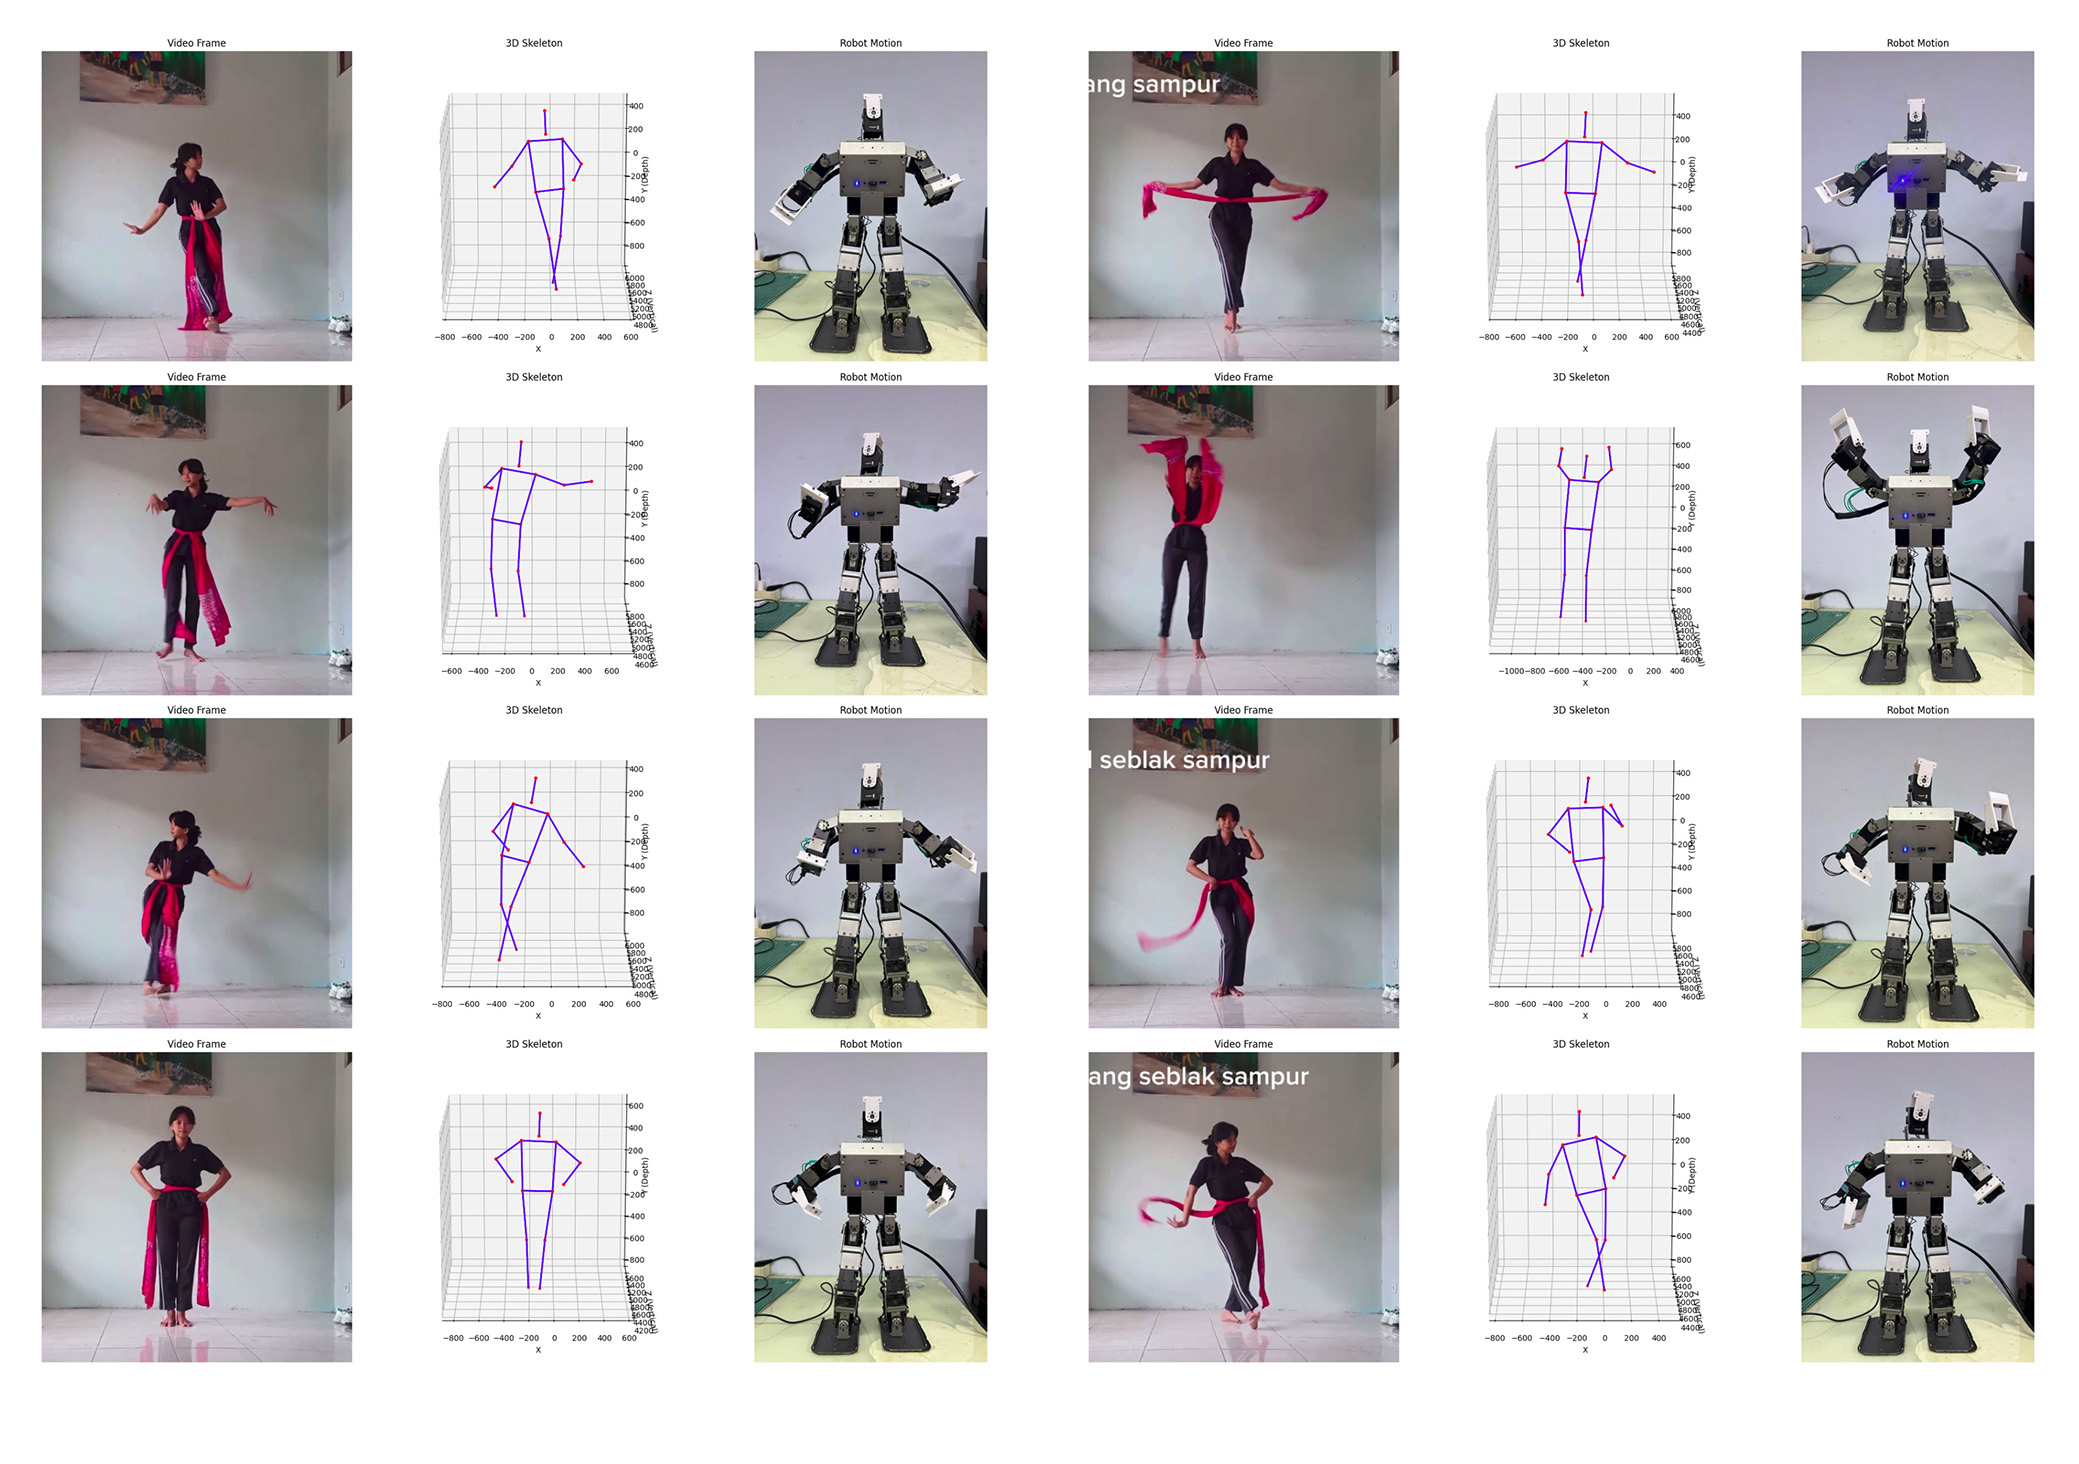
\includegraphics[width=\textwidth]{images/hasil.jpg}
    \caption{Visualisasi motion imitation pada gerakan tari tradisional: frame video asli, rangka hasil estimasi 3D, dan gerakan robot}
    \label{fig:motion_imitation_tari}
\end{figure}

Pada Gambar~\ref{fig:motion_imitation_tari}, ditampilkan hasil percobaan \textit{motion imitation} pada gerakan tari tradisional, yaitu tari Denok Semarangan. Robot berhasil menirukan gerakan tari dengan cukup baik, terutama pada pergerakan tangan dan kepala yang menjadi fokus utama dalam penelitian ini. Posisi lengan dan kepala robot mengikuti pola pose dari data rangka secara real-time, dengan pergerakan yang halus dan stabil antar frame.

\begin{figure}[H]
    \centering
    \includegraphics[width=\textwidth]{images/motion_imitation_coverage.png}
    \caption{Visualisasi motion imitation untuk cakupan gerakan: frame video asli, rangka hasil estimasi 3D, dan gerakan robot}
    \label{fig:motion_imitation_coverage}
\end{figure}

Berdasarkan Gambar~\ref{fig:motion_imitation_coverage}, dapat dilihat bahwa robot mampu mengikuti berbagai variasi gerakan dengan baik. Pada pengujian cakupan gerakan, sistem berhasil memetakan gerakan lengan seperti merentang ke samping, mengangkat ke atas, dan mengarah ke depan tanpa melebihi batas pergerakan mekanis robot. Gerakan yang dihasilkan tetap stabil dan tidak terdapat pergerakan yang melebihi limit servo, sehingga sistem berhasil menjaga keamanan aktuator. Hal ini menunjukkan bahwa proses \textit{motion retargeting} telah berhasil menyesuaikan koordinat tubuh manusia dengan batas kemampuan robot ROBOTIS-OP3 secara efektif.

Walaupun terdapat perbedaan proporsi anatomi antara manusia dan robot, sistem tetap mampu menghasilkan gerakan yang menyerupai tari tradisional secara visual. Hasil ini menunjukkan bahwa pipeline mulai dari input video, estimasi rangka 3D, konversi sudut sendi, hingga eksekusi gerakan robot berjalan dengan baik secara \textit{end-to-end}.


\subsection{Hasil dan Pembahasan Fungsional Sistem}

Pengujian fungsional sistem dilakukan untuk memastikan bahwa seluruh fitur utama berjalan sesuai spesifikasi yang telah dirancang. Pengujian telah dilakukan oleh anggota tim robotik terhadap aplikasi yang telah dikembangkan. Terdapat 6 fitur utama dengan total 6 skenario pengujian, dan seluruh skenario berhasil dijalankan tanpa kendala. Persentase keberhasilan pengujian fungsional sistem adalah \(\frac{6}{6} \times 100\% = 100\%\). Dengan demikian, seluruh fitur pada sistem dinyatakan telah memenuhi kebutuhan fungsional sesuai perancangan.

Tabel~\ref{tab:hasil_pengujian_fungsional} berikut menyajikan hasil lengkap pengujian fungsional sistem.


\begin{longtable}{|c|p{2.5cm}|p{3cm}|p{3cm}|p{2.5cm}|}
\caption{Hasil Pengujian Fungsional Sistem} \label{tab:hasil_pengujian_fungsional} \\
\hline
\textbf{No} & \textbf{Fitur} & \textbf{Skenario Pengujian} & \textbf{Hasil Pengujian} & \textbf{Kesimpulan} \\ \hline
\endfirsthead
\hline
\textbf{No} & \textbf{Fitur} & \textbf{Skenario Pengujian} & \textbf{Hasil Pengujian} & \textbf{Kesimpulan} \\ \hline
\endhead

1 & Upload Video & Pengguna mengunggah file video gerakan tari tradisional & File video berhasil diunggah & Berhasil \\ \hline
2 & Estimasi Pose dan Filtering & Pengguna menekan tombol \textit{Start Pose Estimation} & \textit{Pose estimation} berhasil dijalankan & Berhasil \\ \hline
3 & Tampilan Estimasi Pose & Sistem menampilkan skeleton 3D pada setiap frame video & Sistem menampilkan skeleton 3D dari video (frame awal hingga frame akhir) & Berhasil \\ \hline
4 & Status Log & Sistem mencatat proses pada area log setiap tahapannya & Sistem menampilkan setiap proses yang berlangsung & Berhasil \\ \hline
5 & Penyimpanan Data & Pengguna menyimpan hasil estimasi ke dalam file JSON & File estimasi dari setiap frame didapatkan dalam bentuk JSON & Berhasil \\ \hline
6 & Playback Robot & Pengguna menekan tombol \textit{Gerak} untuk menjalankan robot & Robot bergerak sesuai hasil estimasi proses sebelumnya & Berhasil \\ \hline

\end{longtable}
Dari hasil pengujian fungsional, dapat disimpulkan bahwa sistem telah memenuhi seluruh kebutuhan fungsi utama yang dirancang. Proses mulai dari input video, estimasi pose, penyimpanan data, hingga eksekusi gerakan pada robot ROBOTIS-OP3 berhasil dijalankan dengan baik tanpa kendala teknis.

Keberhasilan ini menunjukkan bahwa sistem dapat digunakan sebagai media representasi gerakan tari tradisional secara otomatis melalui robot humanoid. Implementasi \textit{black-box testing} berhasil memvalidasi bahwa alur aplikasi sesuai dengan rancangan antarmuka dan kebutuhan operasional.

\subsection{Hasil dan Pembahasan Performa Model}

Bagian ini menjelaskan hasil pengujian performa model DeciWatch, mencakup proses training, perbandingan performa antar model, serta visualisasi hasil estimasi pose dan pergerakan sudut sendi.

\subsubsection{Proses Pelatihan dan Evaluasi Model}

Model DeciWatch dilatih menggunakan dataset AIST++ dalam dua sesi training dengan total 45 epoch. Tujuan pelatihan adalah untuk meningkatkan akurasi estimasi pose 3D secara temporal dengan mengoreksi prediksi awal dari model baseline. Pelatihan dilakukan dengan GPU NVIDIA RTX 3060 Mobile. Sesi pertama berlangsung selama 20 epoch, sedangkan sesi kedua dilakukan dari epoch ke-21 hingga ke-45 dengan memuat parameter dari sesi sebelumnya.

Selama proses training, dicatat nilai loss dan Mean Per Joint Position Error (MPJPE). MPJPE input berasal dari prediksi awal model SPIN (yang tetap konstan karena tidak dilatih ulang), sedangkan MPJPE output dihasilkan dari model DeciWatch setelah proses filtering temporal.
\begin{enumerate}
    \item {Sesi Pertama (Epoch 1--20)} \\
    Pada sesi pertama, model dilatih selama 20 epoch. Gambar~\ref{fig:loss_lr_epoch_1} menunjukkan penurunan loss secara konsisten seiring dengan penurunan \textit{learning rate} menggunakan skema eksponensial decay sebesar 0{,}95 per epoch.

    \begin{figure}[H]
        \centering
        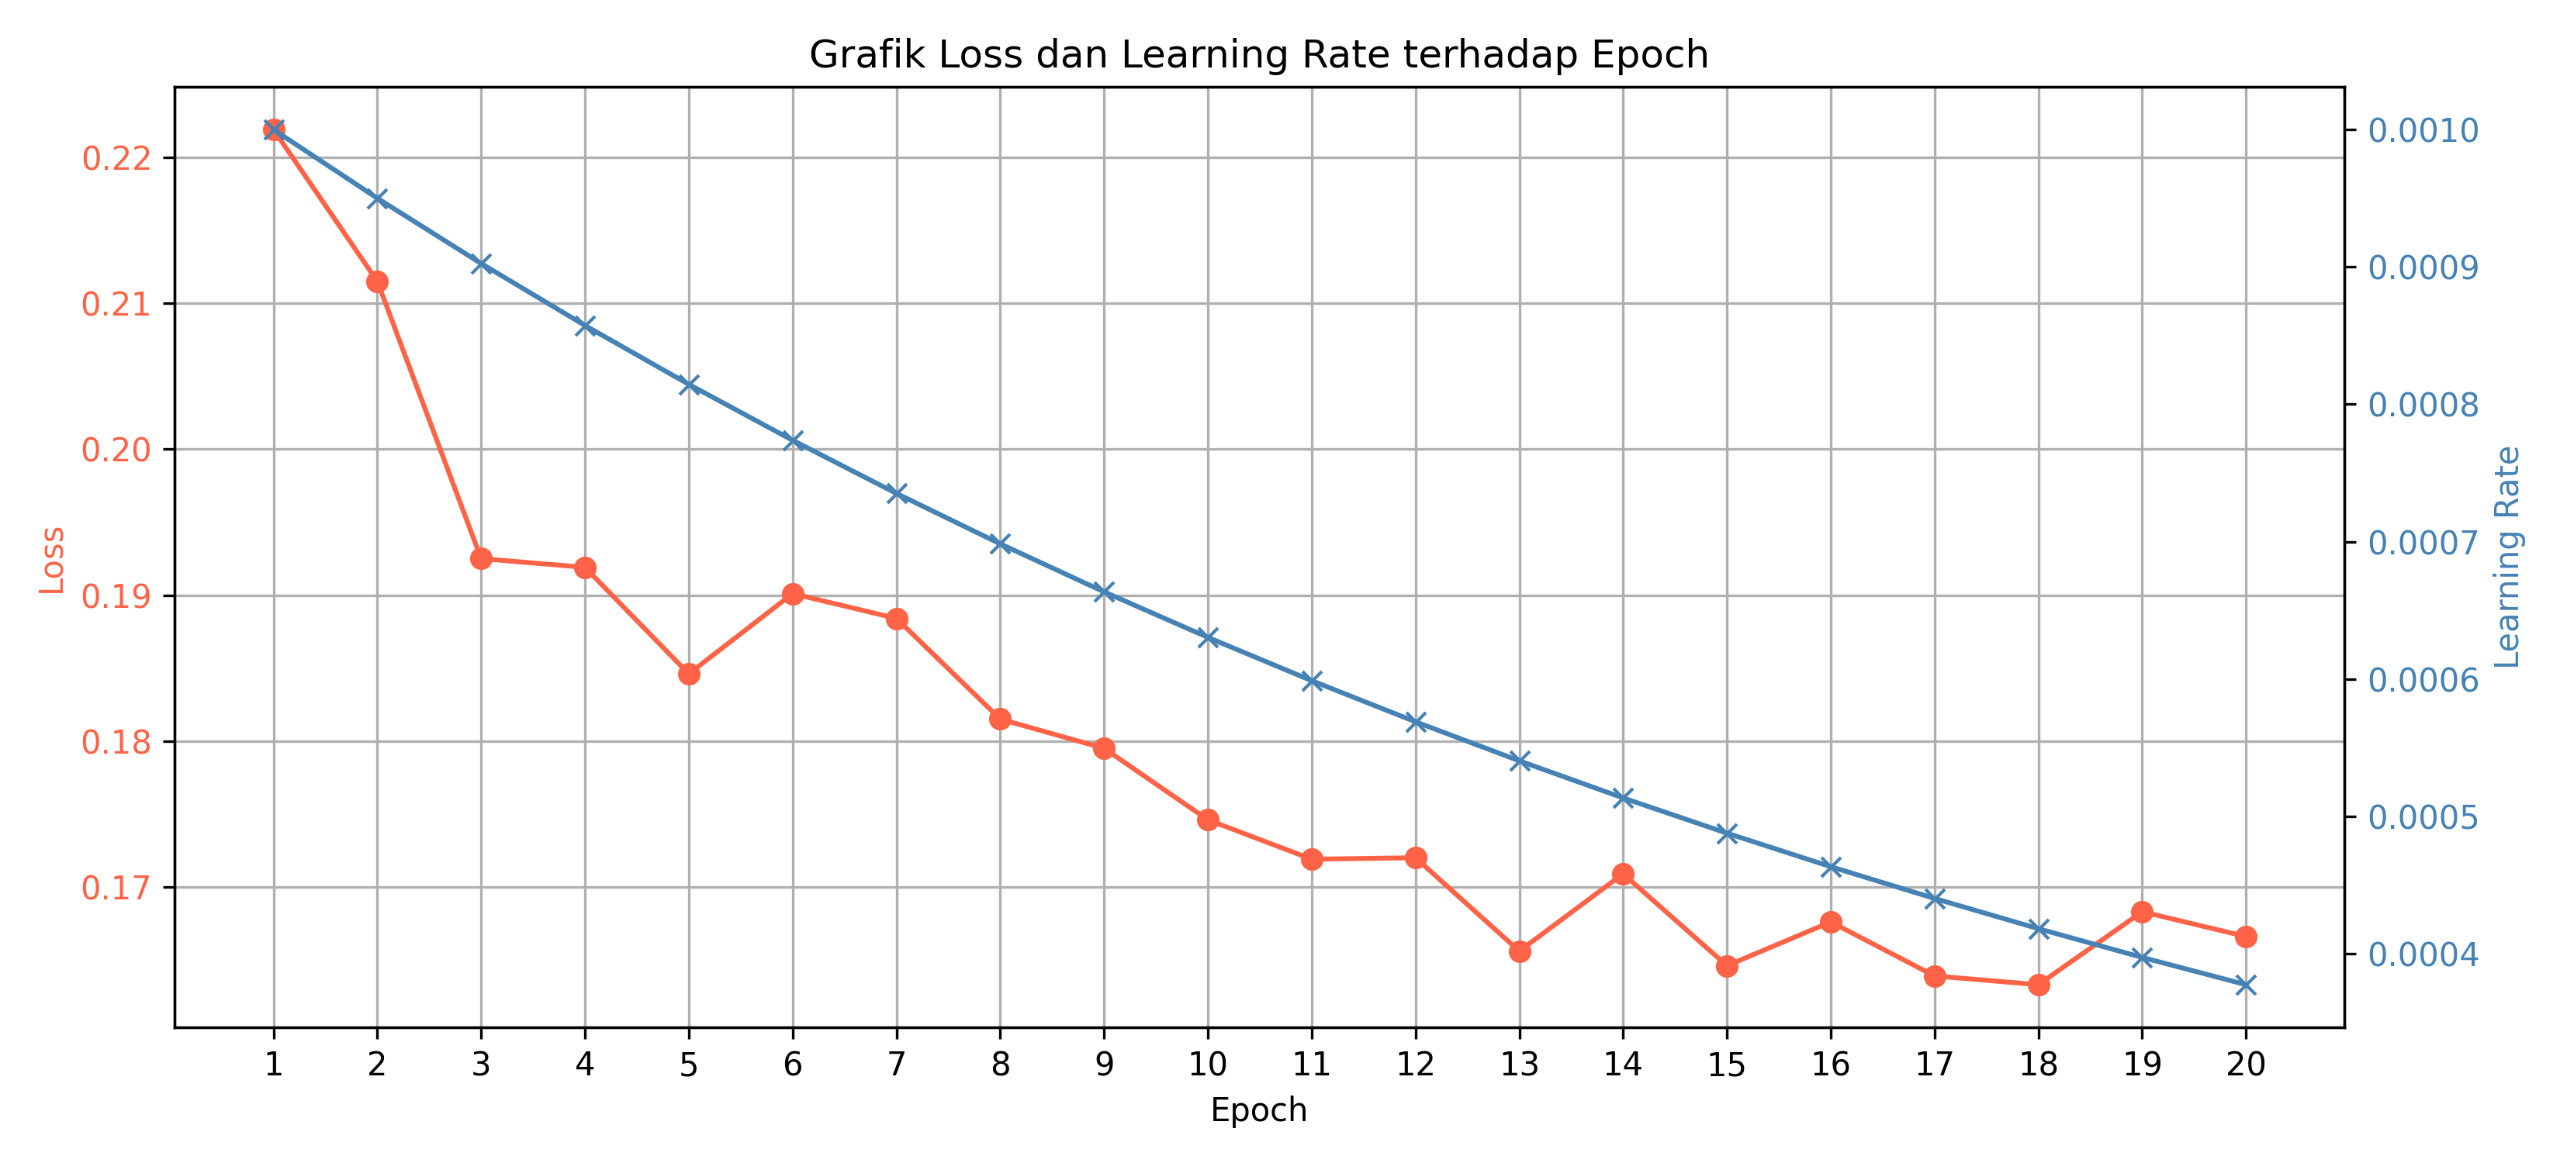
\includegraphics[width=0.9\textwidth]{images/loss_lr_vs_epoch.png}
        \caption{Perbandingan nilai loss dan learning rate terhadap epoch (1--20)}
        \label{fig:loss_lr_epoch_1}
    \end{figure}

    Gambar~\ref{fig:mpjpe_epoch_1} memperlihatkan tren penurunan MPJPE output secara bertahap, sementara MPJPE input tetap konstan. Hal ini menunjukkan bahwa DeciWatch mulai berhasil mengurangi error prediksi pada sesi pertama.

    \begin{figure}[H]
        \centering
        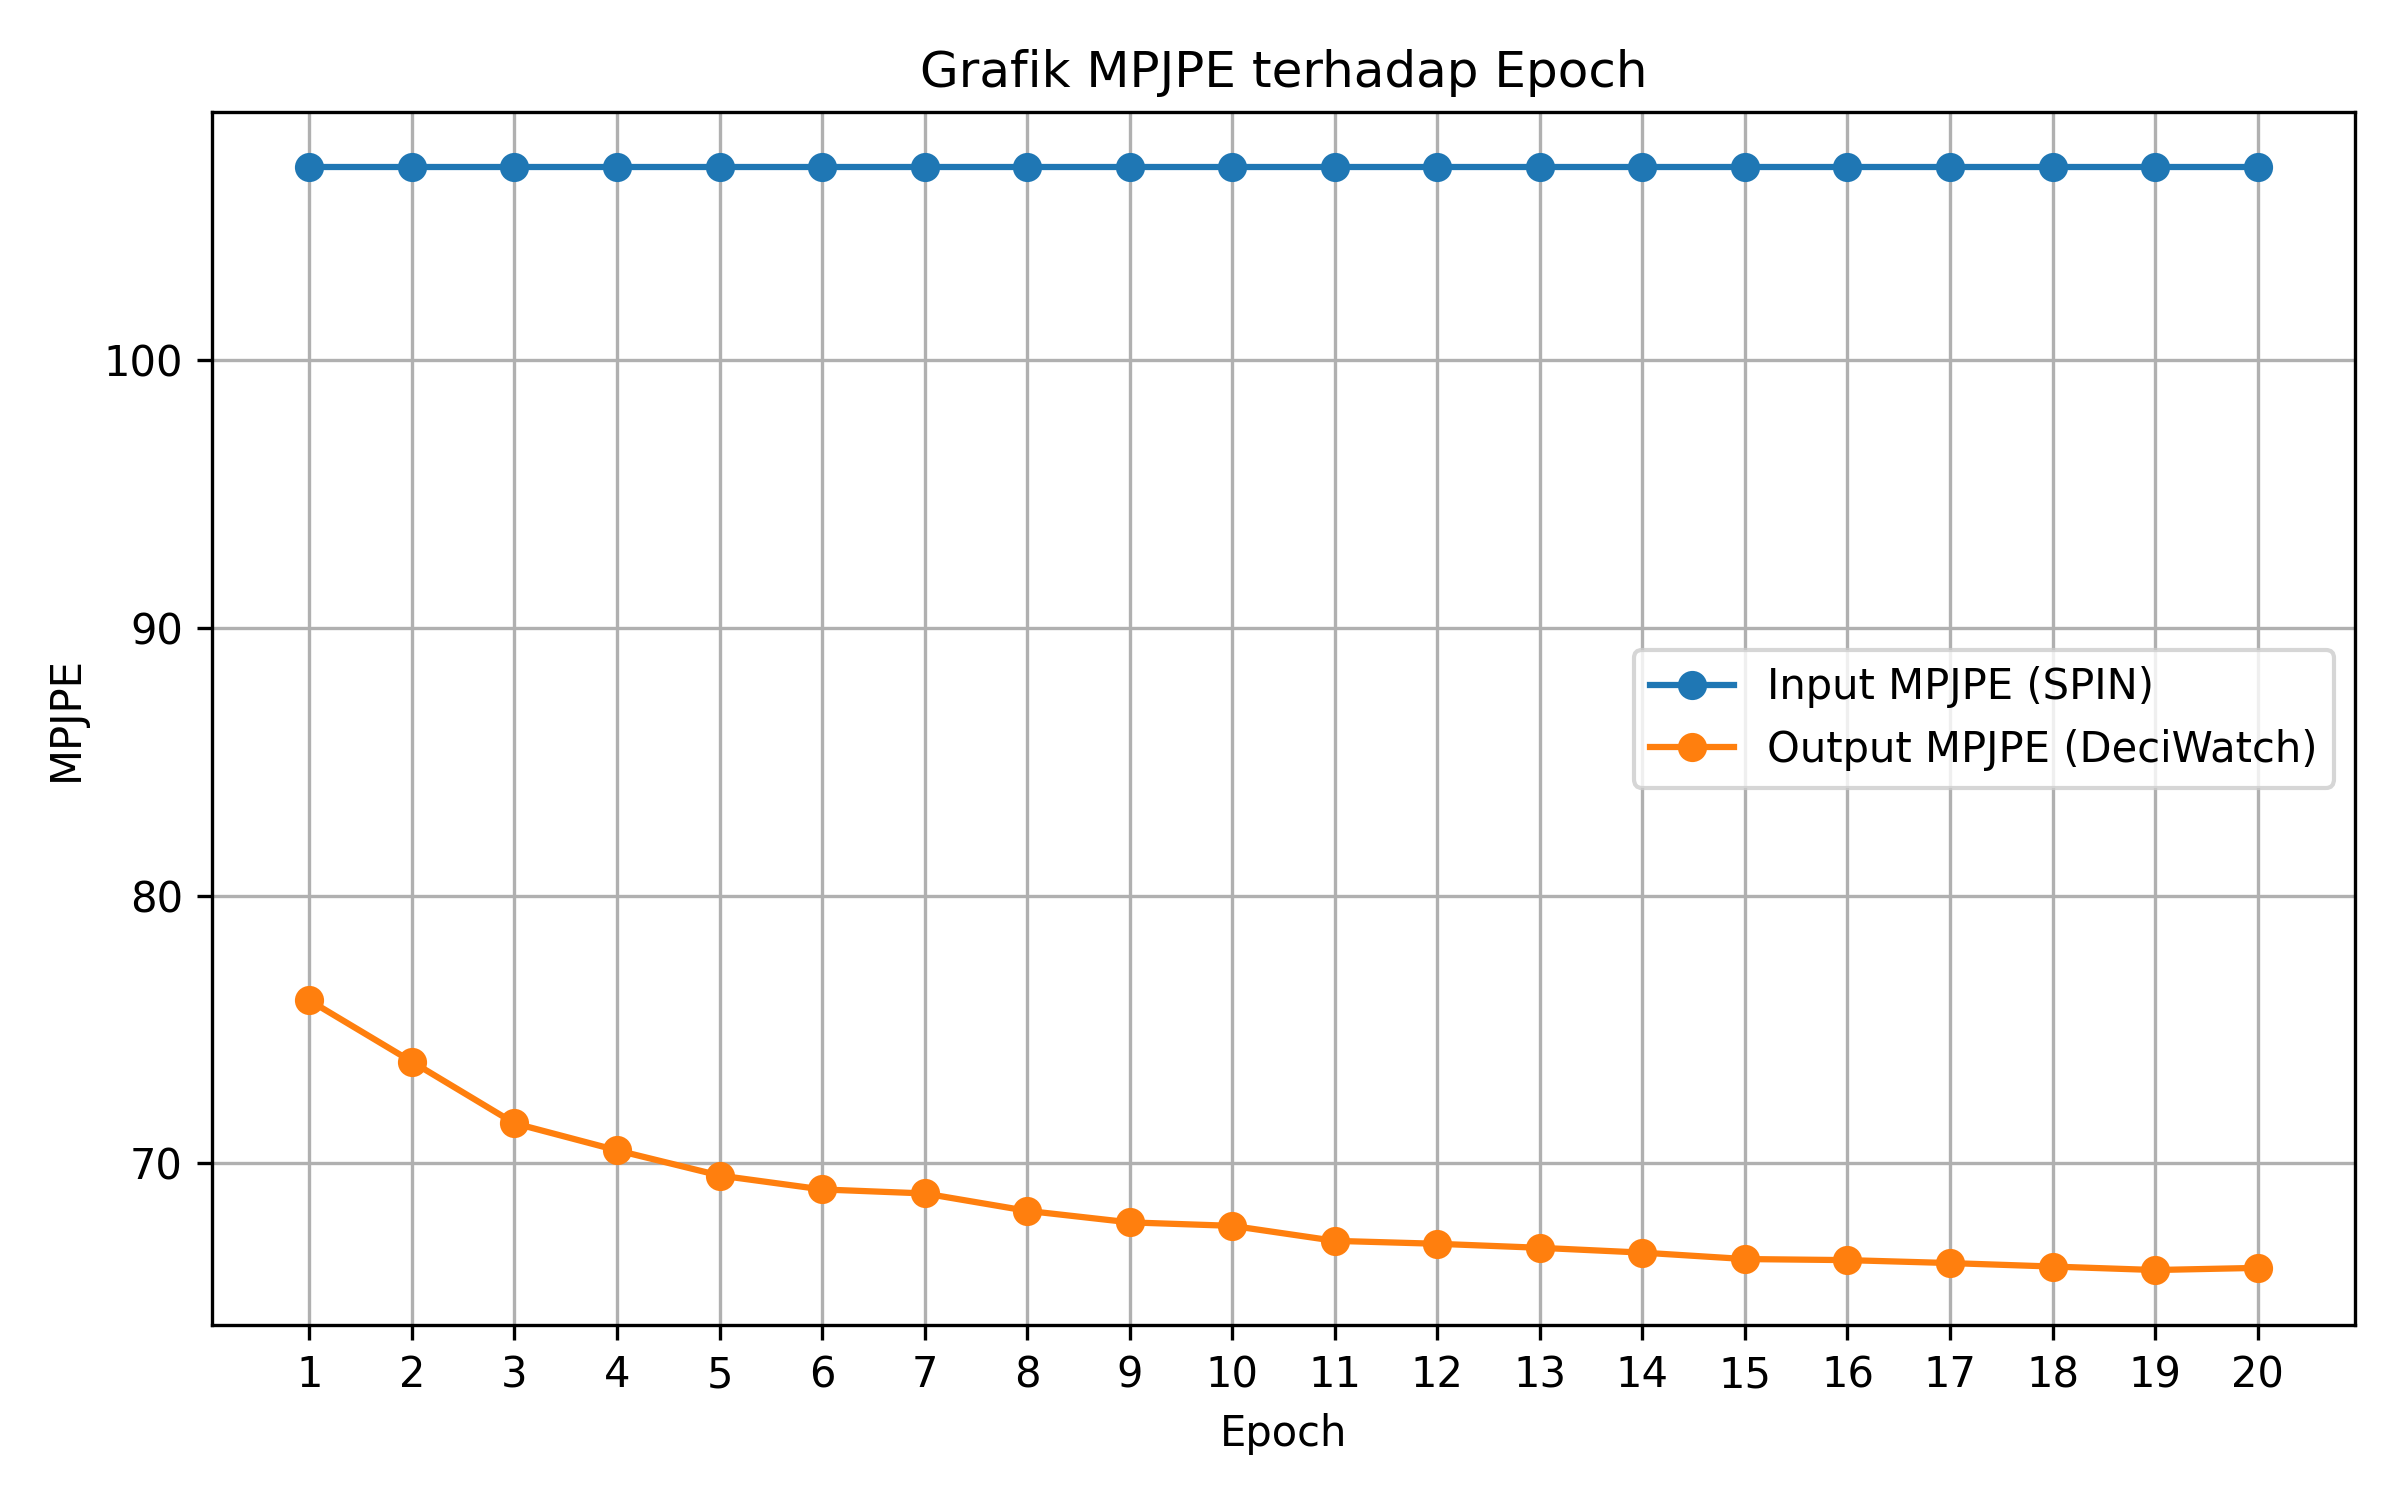
\includegraphics[width=0.9\textwidth]{images/mpjpe_vs_epoch.png}
        \caption{Perbandingan MPJPE antara input dan output pada sesi pelatihan pertama}
        \label{fig:mpjpe_epoch_1}
    \end{figure}

    \item {Sesi Kedua (Epoch 21--45)} \\
    Pada sesi kedua, proses pelatihan dilanjutkan dengan memuat parameter dari sesi pertama. Gambar~\ref{fig:loss_lr_epoch_2} menunjukkan bahwa penurunan loss tetap berlanjut, meskipun laju penurunannya lebih kecil karena \textit{learning rate} terus berkurang.

    \begin{figure}[H]
        \centering
        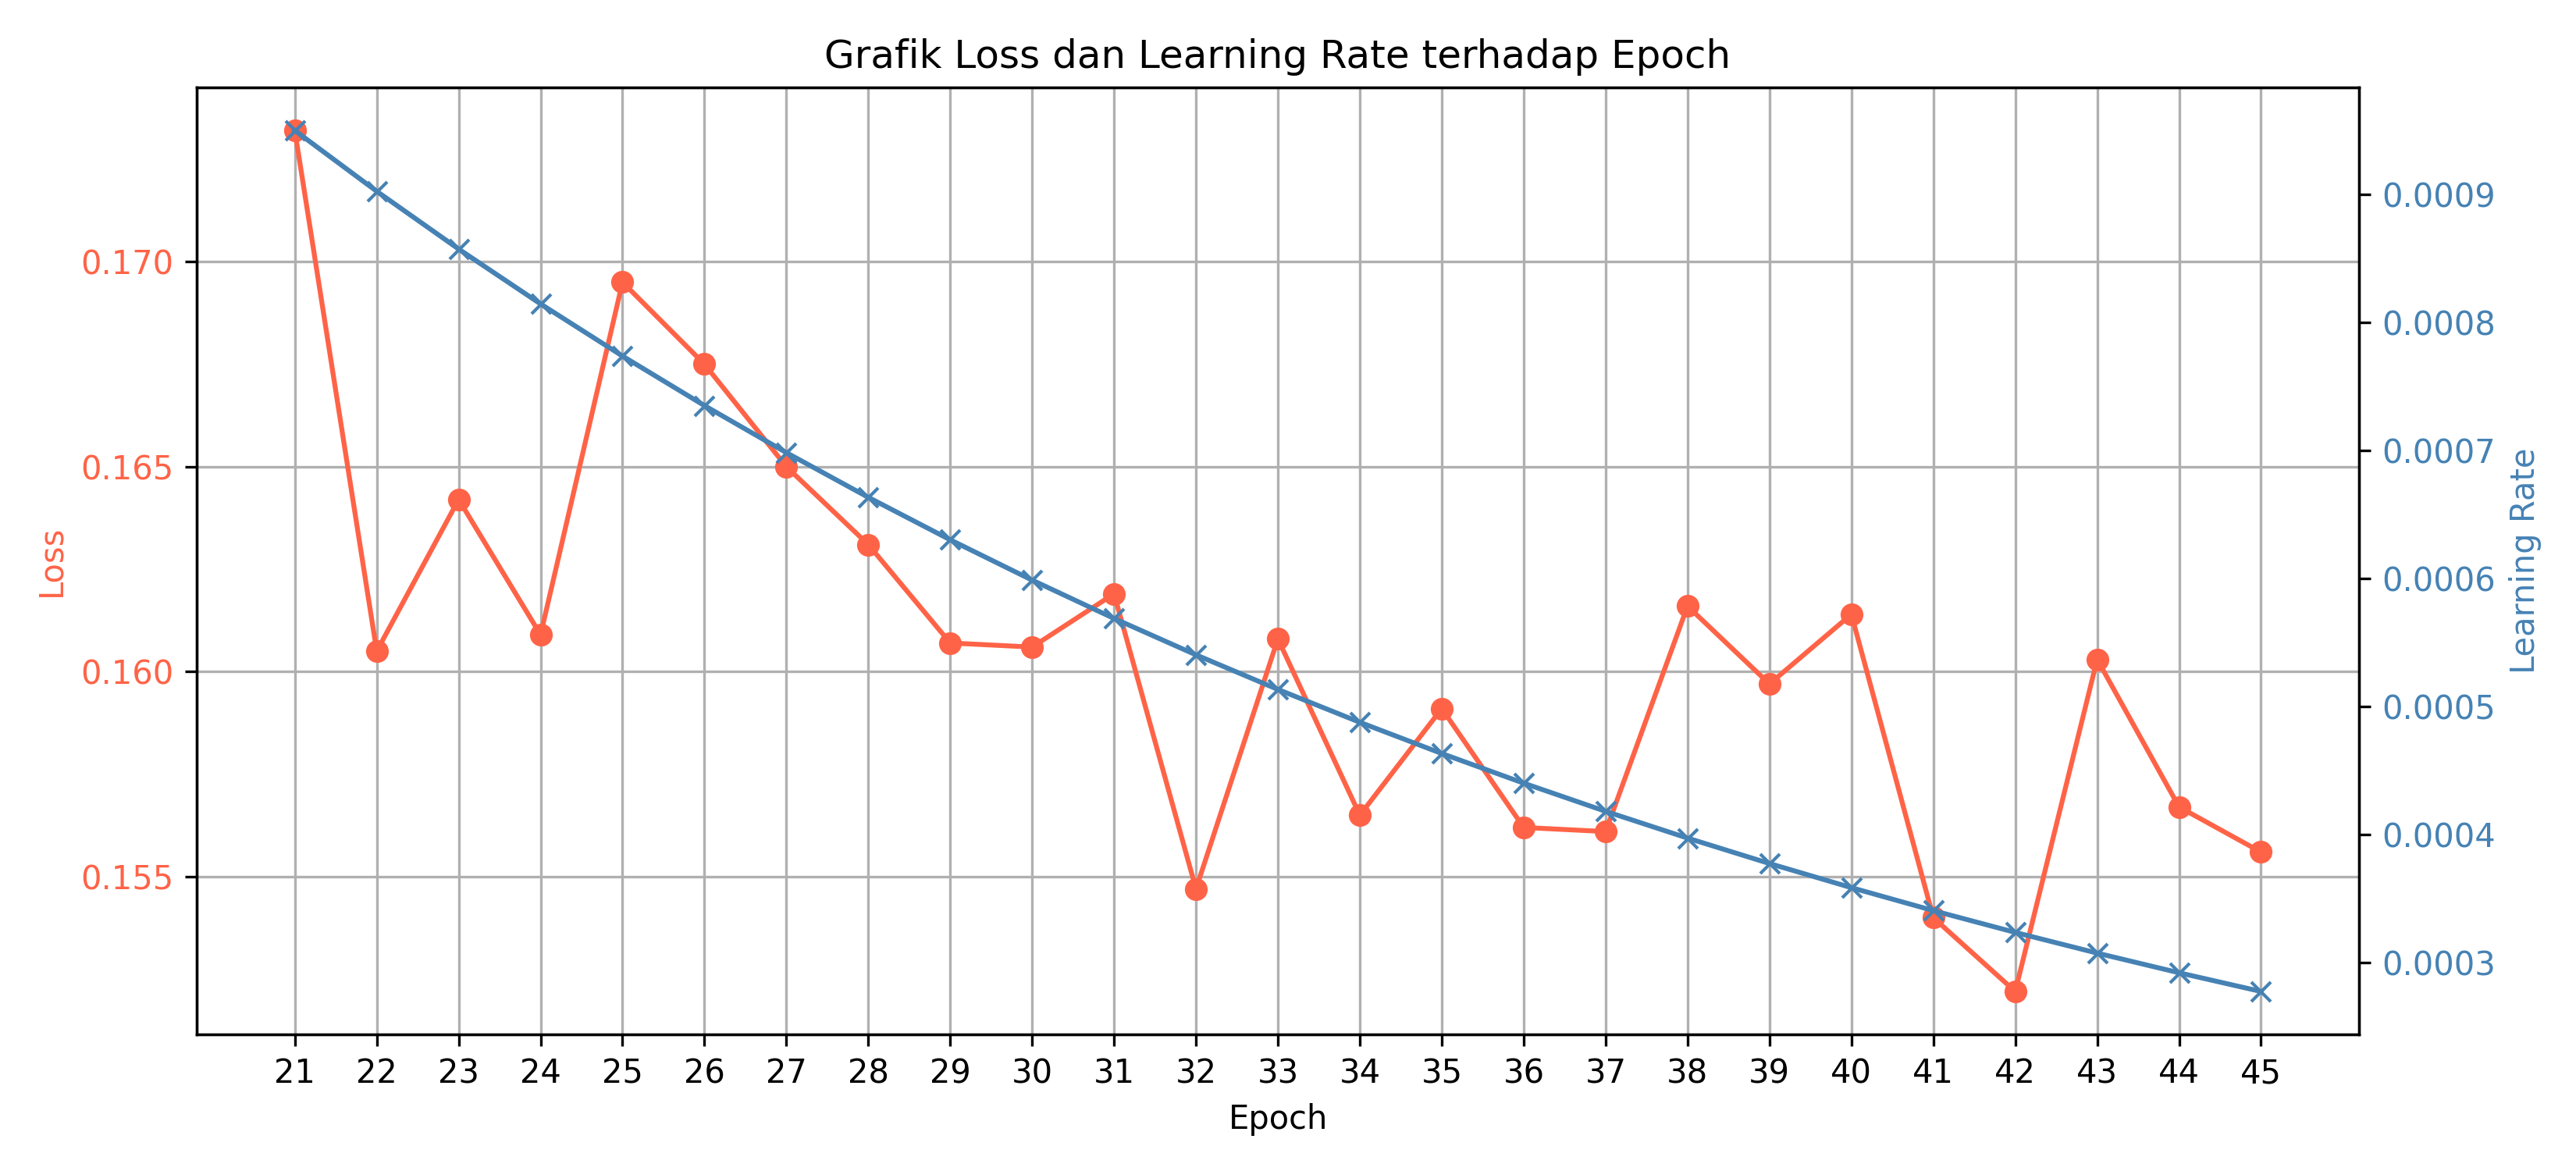
\includegraphics[width=0.9\textwidth]{images/loss_lr_vs_epoch_2.png}
        \caption{Perbandingan nilai loss dan learning rate terhadap epoch (21--45)}
        \label{fig:loss_lr_epoch_2}
    \end{figure}

    Gambar~\ref{fig:mpjpe_epoch_2} memperlihatkan penurunan MPJPE output yang konsisten hingga epoch ke-45. Ini menunjukkan bahwa model semakin mampu mengoreksi kesalahan prediksi secara temporal.

    \begin{figure}[H]
        \centering
        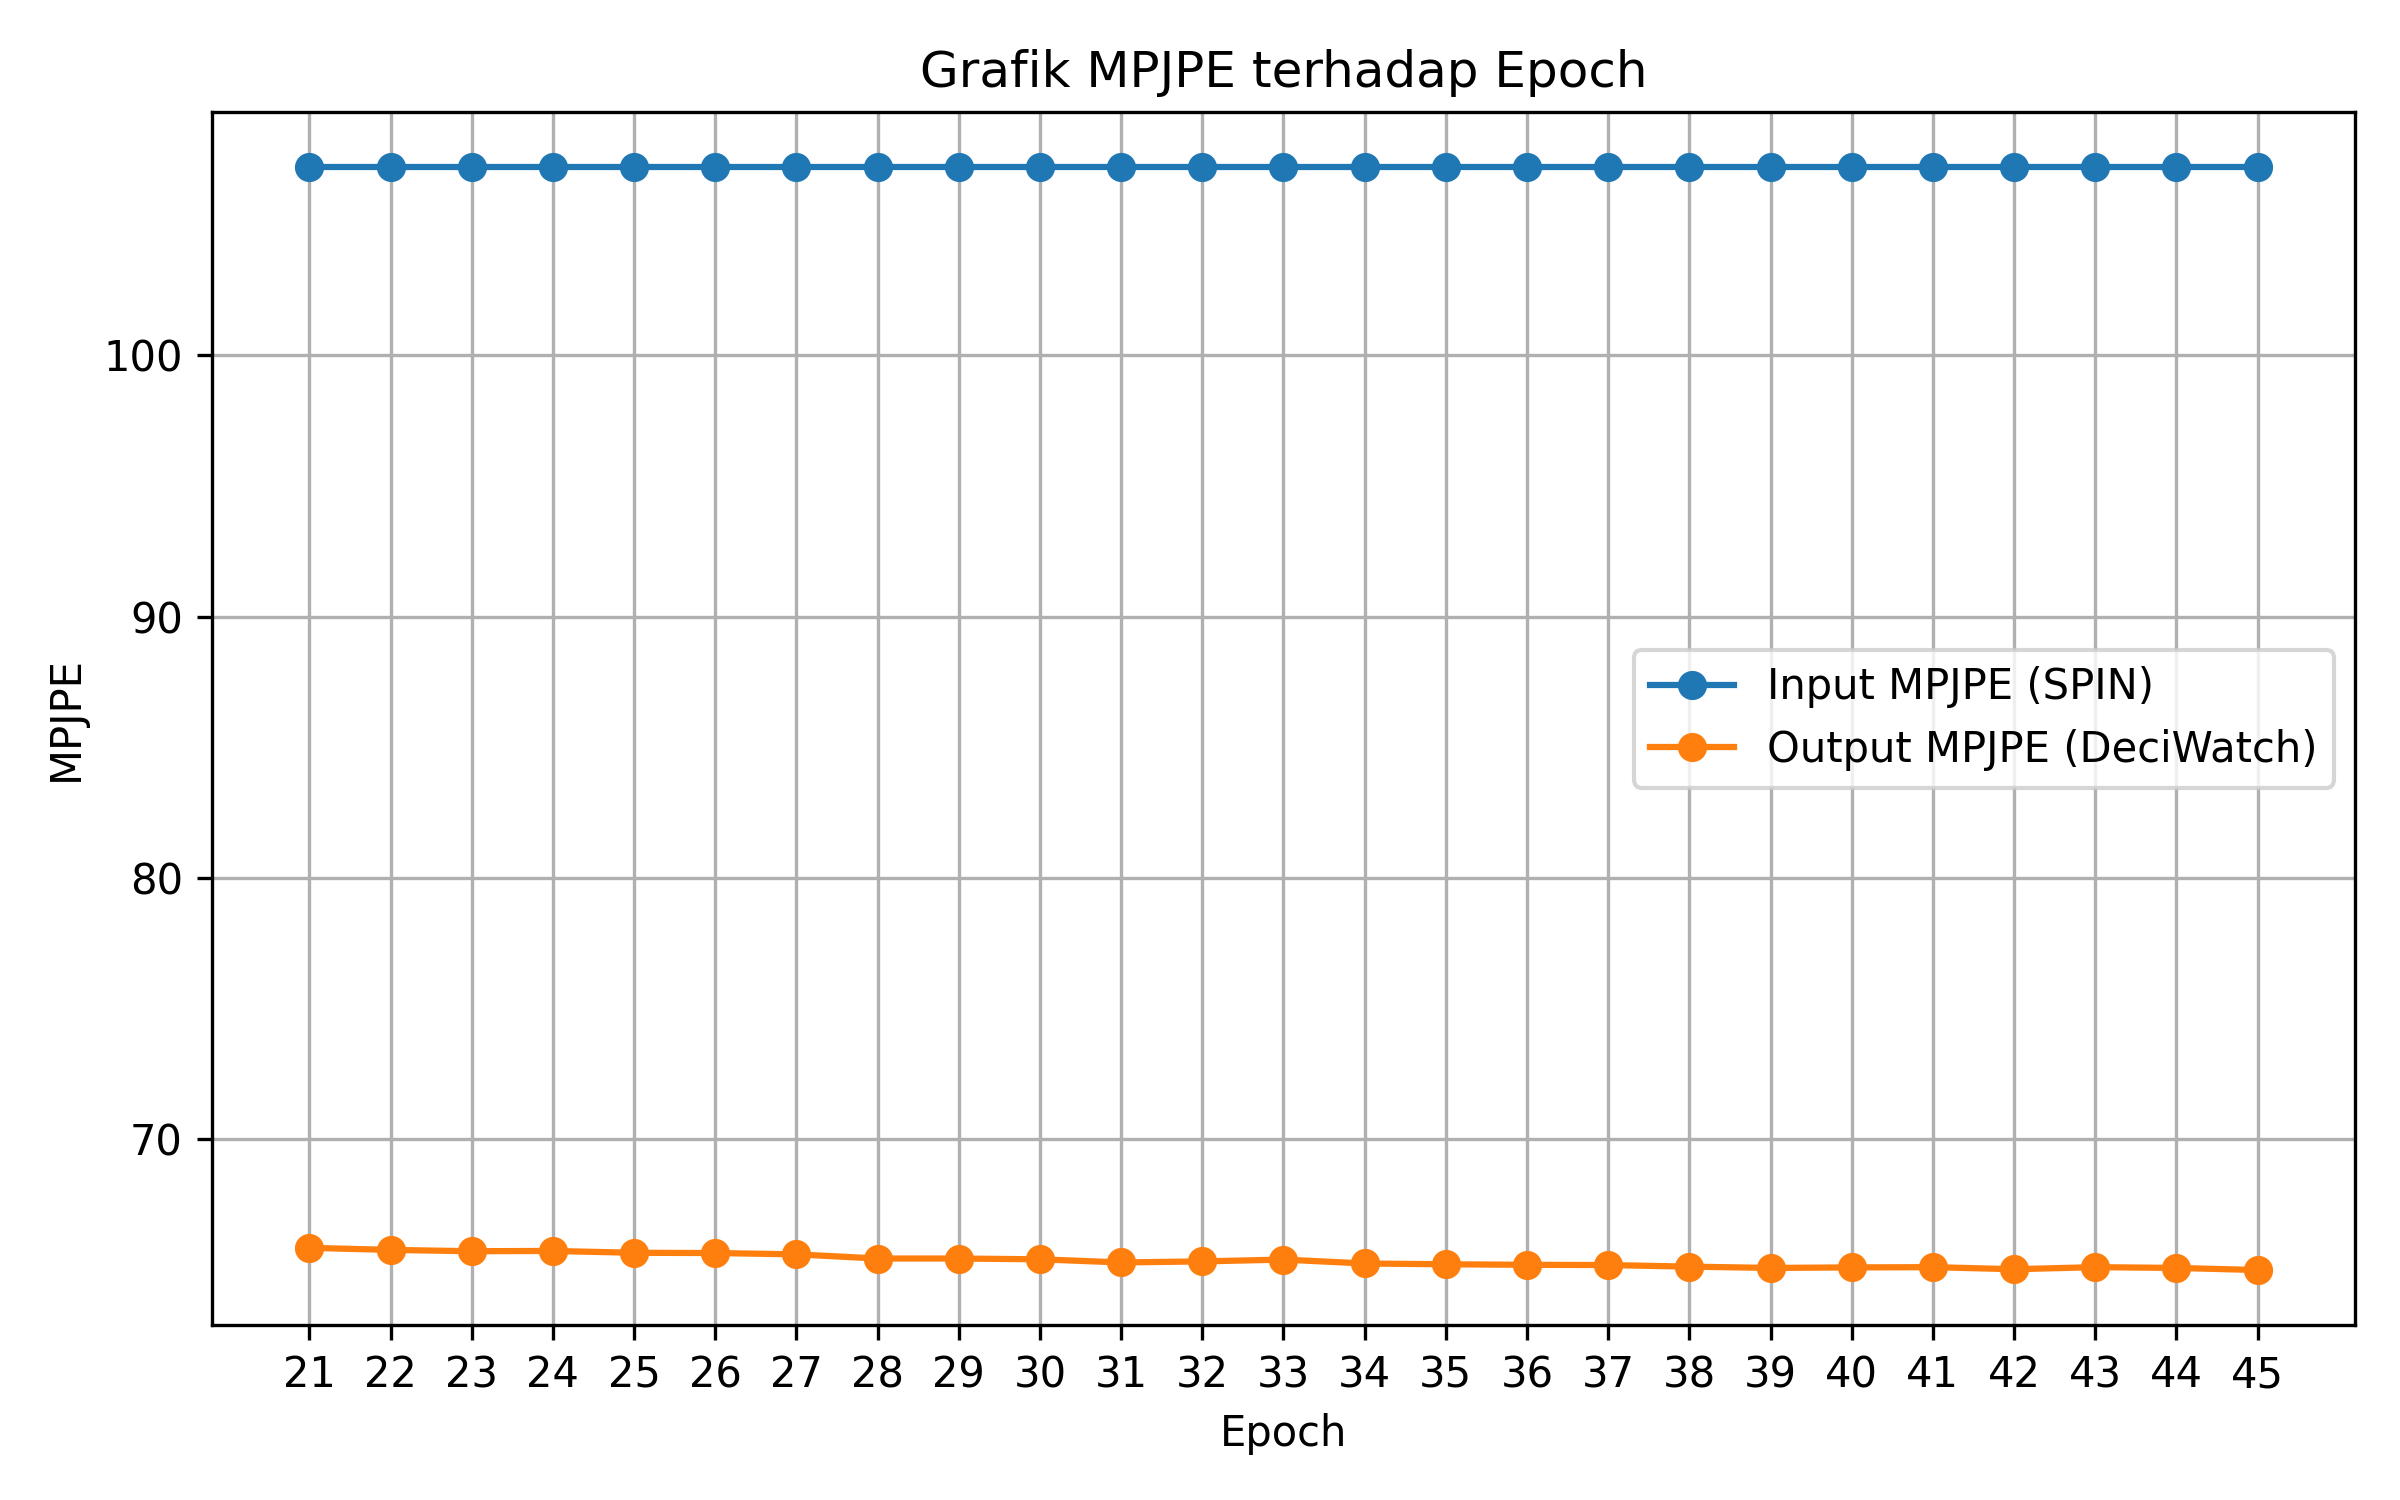
\includegraphics[width=0.9\textwidth]{images/mpjpe_vs_epoch_2.png}
        \caption{Perbandingan MPJPE antara input dan output pada sesi pelatihan kedua}
        \label{fig:mpjpe_epoch_2}
    \end{figure}
\end{enumerate}

Tabel~\ref{tab:hasil_training} merangkum hasil akhir dari dua sesi training, termasuk MPJPE output, loss akhir, dan durasi pelatihan. Berdasarkan tabel tersebut, dapat dilihat bahwa model berhasil menurunkan MPJPE output dari 66{,}10 mm menjadi 64{,}98 mm dengan penurunan loss dari 0{,}1666 ke 0{,}1522 selama dua sesi pelatihan.

\begin{table}[H]
\centering
\caption{Ringkasan Hasil Pengujian Training Model DeciWatch}
\label{tab:hasil_training}
\begin{tabular}{|c|c|c|c|c|}
\hline
\textbf{Sesi} & \textbf{Epoch} & \textbf{MPJPE Output (mm)} & \textbf{Loss Akhir} & \textbf{Durasi Training} \\ \hline
1 & 1--20  & 66.10 & 0.1666 & 24 jam \\ \hline
2 & 21--45 & 64.98 & 0.1522 & 26 jam \\ \hline
\end{tabular}
\end{table}




\subsubsection{Visualisasi Perbandingan Koordinat 3D}
Visualisasi hasil prediksi dilakukan untuk membandingkan koordinat 3D antara model baseline (Metrabs) dan DeciWatch. Grafik berikut menunjukkan perbandingan koordinat X, Y, dan Z untuk beberapa joint seperti pergelangan tangan kanan (\textit{rwrist}), pergelakngan tangan kiri (\textit{lwrist}), dan kepala (\textit{head}).

\begin{figure}[H]
    \centering
    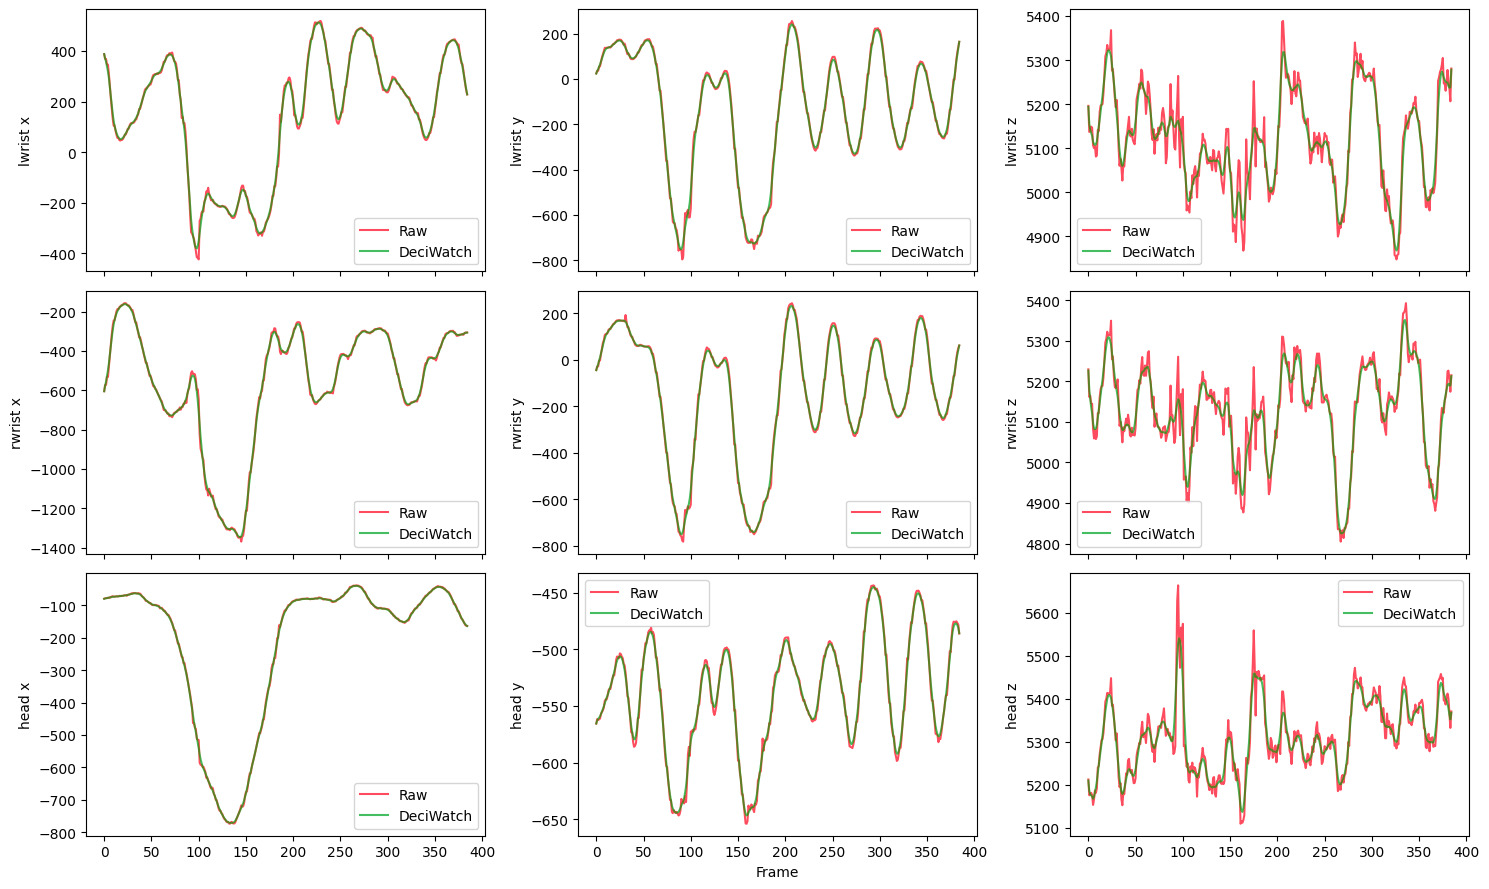
\includegraphics[width=\textwidth]{images/koordinat_per_joint.png}
    \caption{Perbandingan koordinat X, Y, dan Z hasil estimasi pose 3D antara Metrabs (\textit{Raw}) dan DeciWatch (\textit{Filtered})}
    \label{fig:koordinat_joint}
\end{figure}

Kurva berwarna merah menunjukkan data mentah dari Metrabs, sedangkan kurva hijau menunjukkan hasil DeciWatch. Berdasarkan visualisasi tersebut, dapat dilihat bahwa pada data mentah (\textit{Raw}), khususnya pada sumbu Z, terdapat fluktuasi yang lebih signifikan dibandingkan sumbu X dan Y. Hal ini disebabkan karena sumbu Z merepresentasikan kedalaman (\textit{depth}), yang merupakan komponen paling sulit diprediksi dari input 2D. Model estimasi pose seperti Metrabs harus mengonversi informasi gambar dua dimensi menjadi prediksi posisi tiga dimensi, sehingga prediksi pada sumbu Z cenderung lebih rentan terhadap noise.

Dengan penerapan DeciWatch sebagai model \textit{temporal filter}, noise pada sumbu Z berhasil direduksi secara signifikan. DeciWatch memanfaatkan konteks waktu untuk melakukan \textit{smoothing} pada urutan pose, sehingga menghasilkan data gerakan yang lebih halus dan stabil. Hal ini penting agar proses konversi ke sudut sendi (melalui \textit{inverse kinematics}) menjadi lebih akurat dan menghindari gerakan robot yang tidak realistis akibat data yang terlalu berfluktuasi.


\subsubsection{Perbandingan Model Custom dan Pre-trained}

Pengujian dilakukan untuk membandingkan performa model DeciWatch hasil training custom dengan model pre-trained bawaan DeciWatch. Model custom menggunakan \textit{skip frame} 5, sedangkan model pre-trained menggunakan nilai default 10.

Hasil perbandingan menunjukkan bahwa model custom memiliki MPJPE output lebih rendah, yaitu 64{,}98 mm dibandingkan pre-trained sebesar 71{,}27 mm. Hal ini disebabkan oleh resolusi temporal yang lebih rapat pada model custom, sehingga mampu mempelajari variasi gerakan secara lebih detail.

Tabel~\ref{tab:perbandingan_model} menunjukkan perbandingan performa kedua model.

\begin{table}[H]
\centering
\caption{Perbandingan Performa Model Custom dan Model Pre-trained}
\label{tab:perbandingan_model}
\begin{tabular}{|c|c|c|c|}
\hline
\textbf{Model} & \textbf{MPJPE Output (mm)} & \textbf{Loss Akhir} & \textbf{Durasi Training} \\ \hline
Custom Training & 64.98 & 0.1522 & 50 jam \\ \hline
Pre-trained & 71.27 & - & - \\ \hline
\end{tabular}
\end{table}

Hasil ini menunjukkan bahwa proses training yang disesuaikan dengan konfigurasi dataset yang berupa data dance, memiliki gerakan yang cepat dan lambat dan parameter temporal dapat meningkatkan akurasi estimasi pose 3D dibandingkan dengan model pre-trained standar.


    \chapter{KESIMPULAN DAN SARAN}
\vspace{1em}

\section{Kesimpulan}
Berdasarkan hasil penelitian yang berjudul \textit{“Implementasi Pose Estimation untuk Pemodelan Gerak Tari Tradisional Indonesia pada Robot Humanoid ROBOTIS-OP3”}, dapat diambil beberapa kesimpulan sebagai berikut:

\begin{enumerate}
    \item Penelitian ini berhasil mengembangkan sistem estimasi pose 3D berbasis deep learning untuk menganalisis gerakan manusia. Model Metrabs digunakan sebagai baseline untuk deteksi awal pose, sedangkan DeciWatch digunakan untuk menyempurnakan prediksi secara temporal. Hasil pengujian menunjukkan bahwa MPJPE output berhasil diturunkan dari 107 mm (baseline) menjadi 64{,}98 mm setelah proses filtering temporal oleh DeciWatch.
    
    \item Data pose 3D yang dihasilkan berhasil diaplikasikan untuk menggerakkan robot humanoid ROBOTIS-OP3. Proses konversi dari koordinat 3D ke sudut servo dilakukan menggunakan metode \textit{Inverse Kinematics Transform}, sehingga robot mampu menirukan gerakan tari tradisional Indonesia. Pergerakan sudut sendi pada robot menunjukkan perubahan yang kontinu dan relatif halus pada setiap frame, dengan nilai sudut servo yang stabil sesuai data per frame.
    
    \item Aplikasi berbasis website berhasil dirancang dan dibangun untuk mengintegrasikan proses input video, estimasi pose 3D, konversi ke sudut servo, hingga eksekusi gerakan pada robot. Sistem ini memudahkan pengguna dalam mengoperasikan \textit{pipeline} secara terpadu dari antarmuka yang telah disediakan.
    
    \item Model DeciWatch hasil custom training dilatih selama dua sesi dengan total 45 \textit{epoch}, menghasilkan penurunan \textit{loss} dari 0{,}1666 pada sesi pertama menjadi 0{,}1522 pada sesi kedua. MPJPE output pada sesi pertama adalah 66{,}10 mm, sedangkan pada sesi kedua berhasil turun menjadi 64{,}98 mm dengan durasi total pelatihan 50 jam (24 jam pada sesi pertama dan 26 jam pada sesi kedua). Model custom ini memiliki performa lebih baik dibandingkan model pre-trained DeciWatch, yang memiliki MPJPE output sebesar 71{,}27 mm.
\end{enumerate}


\section{Saran}

Berdasarkan hasil penelitian yang telah dilakukan, masih terdapat beberapa aspek yang dapat ditingkatkan dalam pengembangan sistem estimasi pose dan motion imitation pada penelitian berikutnya. Beberapa saran yang dapat diberikan antara lain:

\begin{enumerate}
    \item Menambah variasi dataset yang digunakan, termasuk data gerakan tari tradisional Indonesia dengan kondisi pencahayaan dan sudut pengambilan gambar yang lebih beragam, agar model lebih robust terhadap variasi lingkungan.
    
    \item Meningkatkan kompleksitas model estimasi pose dengan mengeksplorasi arsitektur lain yang memiliki resolusi temporal lebih tinggi, atau mengkombinasikan beberapa model dalam pendekatan ensemble learning.
    
    \item Mengembangkan metode inverse kinematics yang lebih adaptif terhadap keterbatasan fisik robot, sehingga perbedaan proporsi anatomi antara manusia dan robot dapat diminimalkan, dan hasil gerakan menjadi lebih natural.
    
    \item Melakukan pengujian lebih lanjut pada robot secara langsung dalam durasi lebih panjang untuk mengevaluasi ketahanan sistem kontrol gerakan dan kestabilan servo saat mereplikasi gerakan tari yang dinamis.
\end{enumerate}


    %-----------------------------------------------------------
    % End Daftar masukan untuk Bab
    %===========================================================

    %===========================================================
    % Daftar Pustaka
    %-----------------------------------------------------------
    \renewcommand{\bibname}{DAFTAR PUSTAKA}
    \titleformat{\chapter}[block]{\centering\bfseries\large}{\thesection.}{\enspace}{}{}
    \titlespacing*{\chapter}{0pt}{0pt}{*}

    \bibliography{bibtex/daftar-pustaka}
    %-----------------------------------------------------------
    % End Daftar Pustaka
    %===========================================================
    \clearpage

    \phantomsection
    \lampiran
    \clearpage

\end{document}
